\documentclass[compress,10pt]{beamer}

%==================================================================== 
%--------- Make titlepage
%====================================================================
\title{Stochastic block models for networks}
\subtitle{Applications in ecology}
\date{}
\author{Sophie  Donnet,  
\includegraphics[width= 1cm]{plots/Logo-INRAE},    MIA Paris-Saclay 
\includegraphics[width= 0.5cm]{plots/MIAPS}}
\institute{Aug. 2023}
\titlegraphic{\hfill
\includegraphics[width= 0.3  \textwidth]{plots/Logo-INRAE}}


%====================================================================
%---- OPtions 
%====================================================================

%---------------------------------------------------------------- 
%------------    Packages
%-------------------------------------------------------------------------------

\usepackage[T1]{fontenc}
\usepackage[utf8]{inputenc}
\usepackage[english]{babel}
\usepackage{rotating}
\usepackage{graphicx,cancel}
\usepackage{xcolor,colortbl}
\usepackage{subfig} 
\usepackage{amsmath, setspace, amsfonts, amssymb, graphics,multirow}
\usepackage{lmodern}	
\usepackage{array}
\usepackage{mdframed}


%---------------------------------------------------------
%-------------- BEAMER options
%-------------------------------------------------------
\usetheme[outer/progressbar=foot]{metropolis}
\setbeamertemplate{section in toc}[sections numbered]
\setbeamertemplate{subsection in toc}[subsections numbered]

\setbeamerfont{bibliography item}{size=\tiny}
\setbeamerfont{bibliography entry author}{size=\tiny}
\setbeamerfont{bibliography entry title}{size=\tiny}
\setbeamerfont{bibliography entry location}{size=\tiny}
\setbeamerfont{bibliography entry note}{size=\tiny}
            

\definecolor{dgreen2}{RGB}{102,193,191}
\definecolor{dgreen}{RGB}{255,165,0}
\definecolor{mygreen}{RGB}{255,165,0}
\definecolor{mygrey}{RGB}{230,230,230}
\definecolor{links}{HTML}{3D24D1}
\hypersetup{colorlinks,linkcolor=,urlcolor=links}

\setbeamertemplate{blocks}[rounded][shadow=true]
\setbeamercolor{block title}{use = structure  ,bg=mygrey, fg=dgreen}
%\setbeamercolor{normal text}{fg=black,bg=white}
%\setbeamercolor{alerted text}{fg=lgreen}
%\setbeamercolor{example text}{fg=lgreen}
%\setbeamercolor{structure}{fg=dgreen} %d'où ce bleu par défaut
\setbeamercolor{background canvas}{parent=normal text}
\setbeamertemplate{frametitlecontinuation}{\insertcontinuationcountroman}


\AtBeginSection[]
{  \begin{frame}
  \frametitle{}
  \tableofcontents[currentsection, hideothersubsections]
  \end{frame} 
}
  \AtBeginSubsection[]
  {  \begin{frame}
    \frametitle{}
    \tableofcontents[currentsubsection, currentsection,hideothersubsections, subsectionstyle=show/shaded/hide]
    \end{frame} 
  }

  
%-------------------------------------------------------------------------------
%---------------------------- tikz
%-------------------------------------------------------------------------------
\usepackage{tikz}
\usetikzlibrary{calc,shapes,backgrounds,arrows,automata,shadows,positioning}



\newcommand{\nodesize}{1.5em}
\newcommand{\edgeunit}{2*\nodesize}
\tikzstyle{hidden}=[draw, circle, fill=gray!50, minimum width=\nodesize, inner sep=0]
\tikzstyle{observed}=[draw, circle, minimum width=\nodesize, inner sep=0]
\tikzstyle{diagobserved}=[draw, circle, minimum width=\nodesize, inner sep=0,color=gray!50]
\tikzstyle{eliminated}=[draw, circle, minimum width=\nodesize, color=gray!50, inner sep=0]
\tikzstyle{empty}=[]
\tikzstyle{arrow}=[->, >=latex, line width=1pt]
\tikzstyle{edge}=[-, line width=1pt]
\tikzstyle{dashedarrow}=[->, >=latex, dashed, line width=1pt]
\tikzstyle{lightarrow}=[->, >=latex, line width=1pt, fill=gray!50, color=gray!50]

 


%-------------------------------------------------------------------------------
% Quelques options pdf
%-------------------------------------------------------------------------------
\hypersetup{
pdfpagemode = FullScreen, % afficher le pdf en plein \'ecran
pdfauthor   = {},%
pdftitle    = {},%
pdfsubject  = {},%
pdfkeywords = {Science,Impact},%
pdfcreator  = {PDFLaTeX,emacs,AucTeX},%
pdfproducer = {INRAE}%
}


\newcommand\Wider[2][3em]{%
\makebox[\linewidth][c]{%
  \begin{minipage}{\dimexpr\textwidth+#1\relax}
  \raggedright#2
  \end{minipage}%
  }%
}



\newcommand{\I}{\mathbb{I}}
\newcommand{\E}{\mathbb{E}}
\renewcommand{\P}{\mathbb{P}}

\DeclareMathOperator*{\argmax}{arg\,max}
\DeclareMathOperator*{\argmin}{arg\,min}
\newcommand{\KL}{\mathrm{KL}}
\newcommand{\ICL}{\mathrm{ICL}}
\newcommand{\pen}{\mathrm{pen}}


\newcommand{\diag}{\mathop{\mathrm{diag}}}
\newcommand{\bbeta}{\boldsymbol{\beta}}
\newcommand{\balpha}{\boldsymbol{\alpha}}
\newcommand{\btheta}{\boldsymbol{\theta}}
\newcommand{\bY}{\mathbf{Y}}
\newcommand{\M}{\mathcal{M}_{\bK}}
\newcommand{\Mcal}{\mathcal{M}}
\newcommand{\bK}{\mathbf{K}}
\newcommand{\bX}{\mathbf{Y}}
\newcommand{\Xall}{\mathbf{Y}}
\newcommand{\Zall}{\mathbf{Z}}
\newcommand{\bpi}{\mathbf{\pi}}
\newcommand{\btau}{\mathbf{\tau}}
\newcommand{\bZ}{\mathbf{Z}}
\newcommand{\by}{\mathbf{y}}
\newcommand{\bz}{\mathbf{z}}
\newcommand{\ba}{\mathbf{a}}
\newcommand{\bt}{\mathbf{t}}
\newcommand{\bx}{\mathbf{x}}
\newcommand{\bh}{\mathbf{h}}
\newcommand{\bb}{\mathbf{b}}
\newcommand{\bB}{\mathbf{B}}
\newcommand{\bC}{\mathbf{C}}
\newcommand{\bM}{\mathbf{M}}
\newcommand{\bphi}{\boldsymbol{\phi}}
\newcommand{\blambda}{\boldsymbol{\lambda}}
\newcommand{\bepsilon}{\boldsymbol{\epsilon}}
\newcommand{\bpsi}{\boldsymbol{\psi}}
\newcommand{\bm}{\mathbf{m}}
\newcommand{\ra}{\bigskip \textcolor{dgreen}{$\rightarrow$}\;}
\newcommand{\btVFill}{\vskip0pt plus 1filll}


 

%====================================================================
\begin{document}
%====================================================================


%====================================================================
\begin{frame}
%====================================================================

\titlepage


\end{frame}

 
%====================================================================
\begin{frame}{My collaborators}
%====================================================================


\alert{On the R packages}

\begin{tabular}{cccc}
 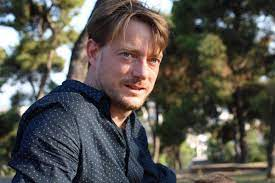
\includegraphics[width = 0.20\textwidth]{plots/Chiquet}& 
\includegraphics[width = 0.20\textwidth]{plots/Barbillon}& 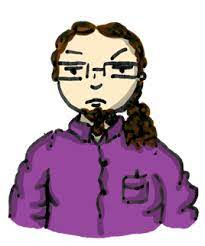
\includegraphics[width = 0.20\linewidth]{plots/jbleger} &
\includegraphics[width = 0.20\textwidth]{plots/saintclair}\\
 \scriptsize J. Chiquet  & \scriptsize P. Barbillon & \scriptsize J.B. Léger & \scriptsize Saint-Clair Chabert-Liddell \\
 \scriptsize (INRAE) & \scriptsize (AgroParisTech) & \scriptsize (Univ. Tech. Compiègne)& \scriptsize (INRAE)\\
 \hline 
 \scriptsize \textsf{sbm}& \scriptsize \textsf{sbm} & \scriptsize \textsf{blockmodels} & \scriptsize  \textsf{colSBM} 
\end{tabular}

\bigskip
\alert{Other collaborators} 

 


T. Vanrenterghem (INRAE), S. Robin (Sorbonne U.),  E. Lazega (Sciences Po),  F. Massol (CNRS), S. Kefi (CNRS) +  \href{https://cmatias.perso.math.cnrs.fr/ANR_EcoNet.html}{ANR Econet} + ANR Pastodiv + GDR Resodiv





\end{frame}


  

%====================================================================
\section{Introduction}
%====================================================================


%===================================================================
\begin{frame} \frametitle{Networks }
%===================================================================

Convenient tools to encode / represent interactions between entities

\begin{center}
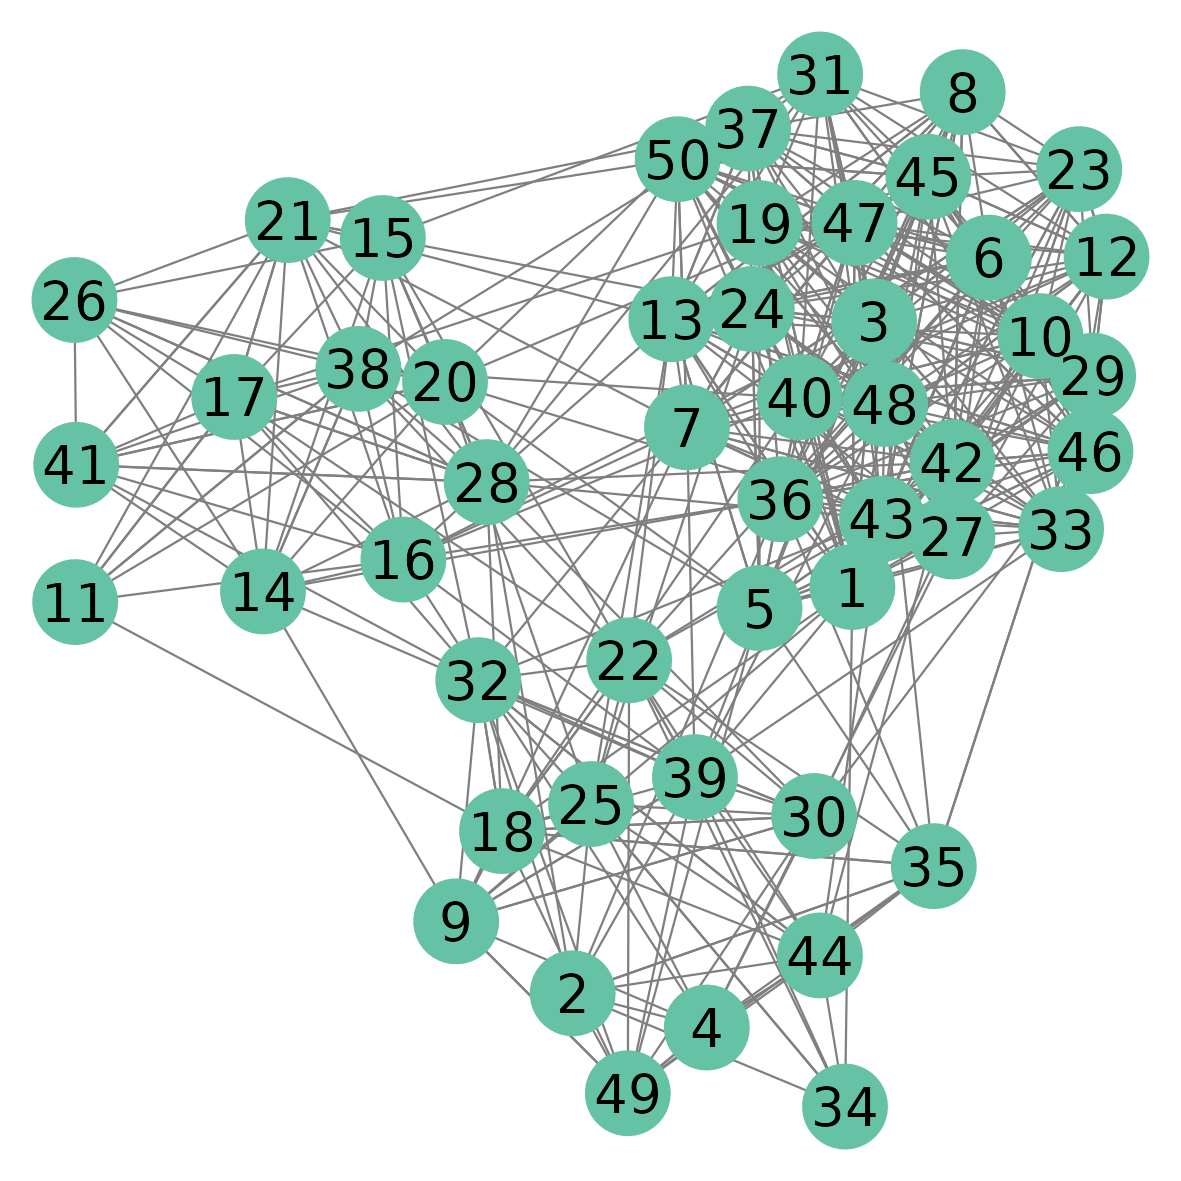
\includegraphics[width=0.4\textwidth]{plots/network_raw.png}
\end{center}


 A network consists in:
 \begin{itemize}
  \item \alert{nodes/vertices} which represent individuals / species / entities which may interact or not,
  \item \alert{links/edges/connections} which stand for an interaction between a pair of nodes / dyads.
  
 \end{itemize}
 
 \end{frame}
 
 

%===================================================================
\begin{frame} \frametitle{Social networks}
%===================================================================
\begin{itemize}
\item Friendship between individuals,  
\includegraphics[width=0.1\textwidth]{plots/facebook.png} 
\item Linkedin 
\includegraphics[width=0.05\textwidth]{plots/linkedIn.png} 
\item Twitter 
\includegraphics[width=0.5cm]{plots/twitter.png}

\item Co-publication between researchers   
\item Advices between lawyers: \alert{oriented relation}
\item \href{https://www.cs.cmu.edu/~./enron/}{Enron email dataset}
\item Exchanges of seeds between farmers  
\end{itemize}


\end{frame}

%====================================================================
\frame{\frametitle{Networks in ecology}
%====================================================================


\begin{itemize}
 \item Ecosystems involve many species 
 \item Interactions between species determine the functioning and evolution of ecosystems
 \item \alert{Several types of interactions}
\end{itemize}

\begin{columns}
\begin{column}{0.33\textwidth}
Predation \\ 

\includegraphics[width=0.9 \textwidth]{plots/predation}
\end{column}
\begin{column}{0.3\textwidth}
Parasitism\\ 
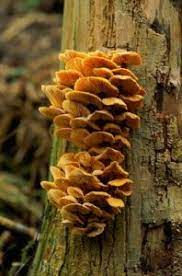
\includegraphics[width= 0.9\textwidth]{plots/parasite}
\end{column}
\begin{column}{0.3\textwidth}
Pollination\\
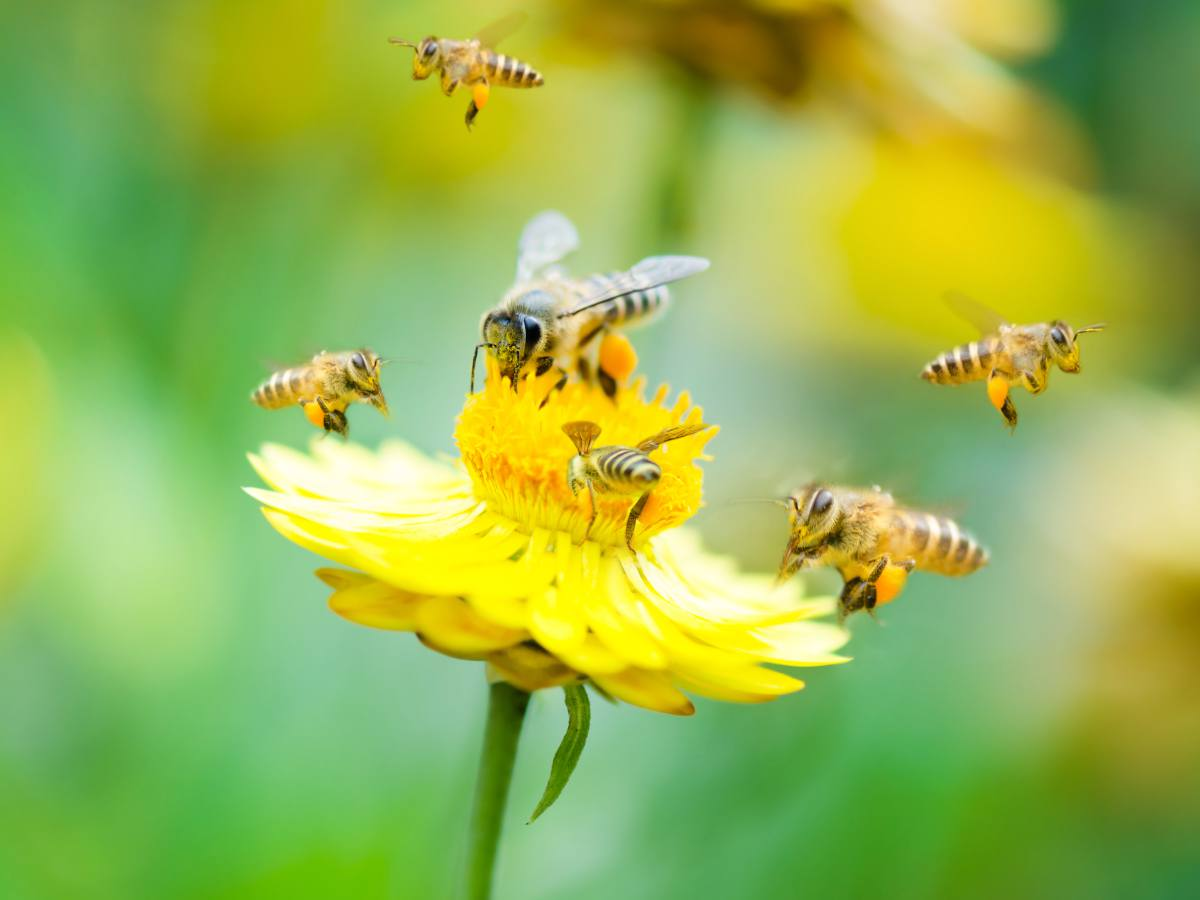
\includegraphics[width= 0.9\textwidth]{plots/pollination}
\end{column}
 \end{columns}
 
}

 

%====================================================================
\frame{\frametitle{Predation networks: foodwebs}
%====================================================================
\textcolor{mygreen}{\cite{thompson2003impacts}} Pine-forest stream foodweb  issued from  North-Caroline    ($71$ species, $148$ interactions)


\centering
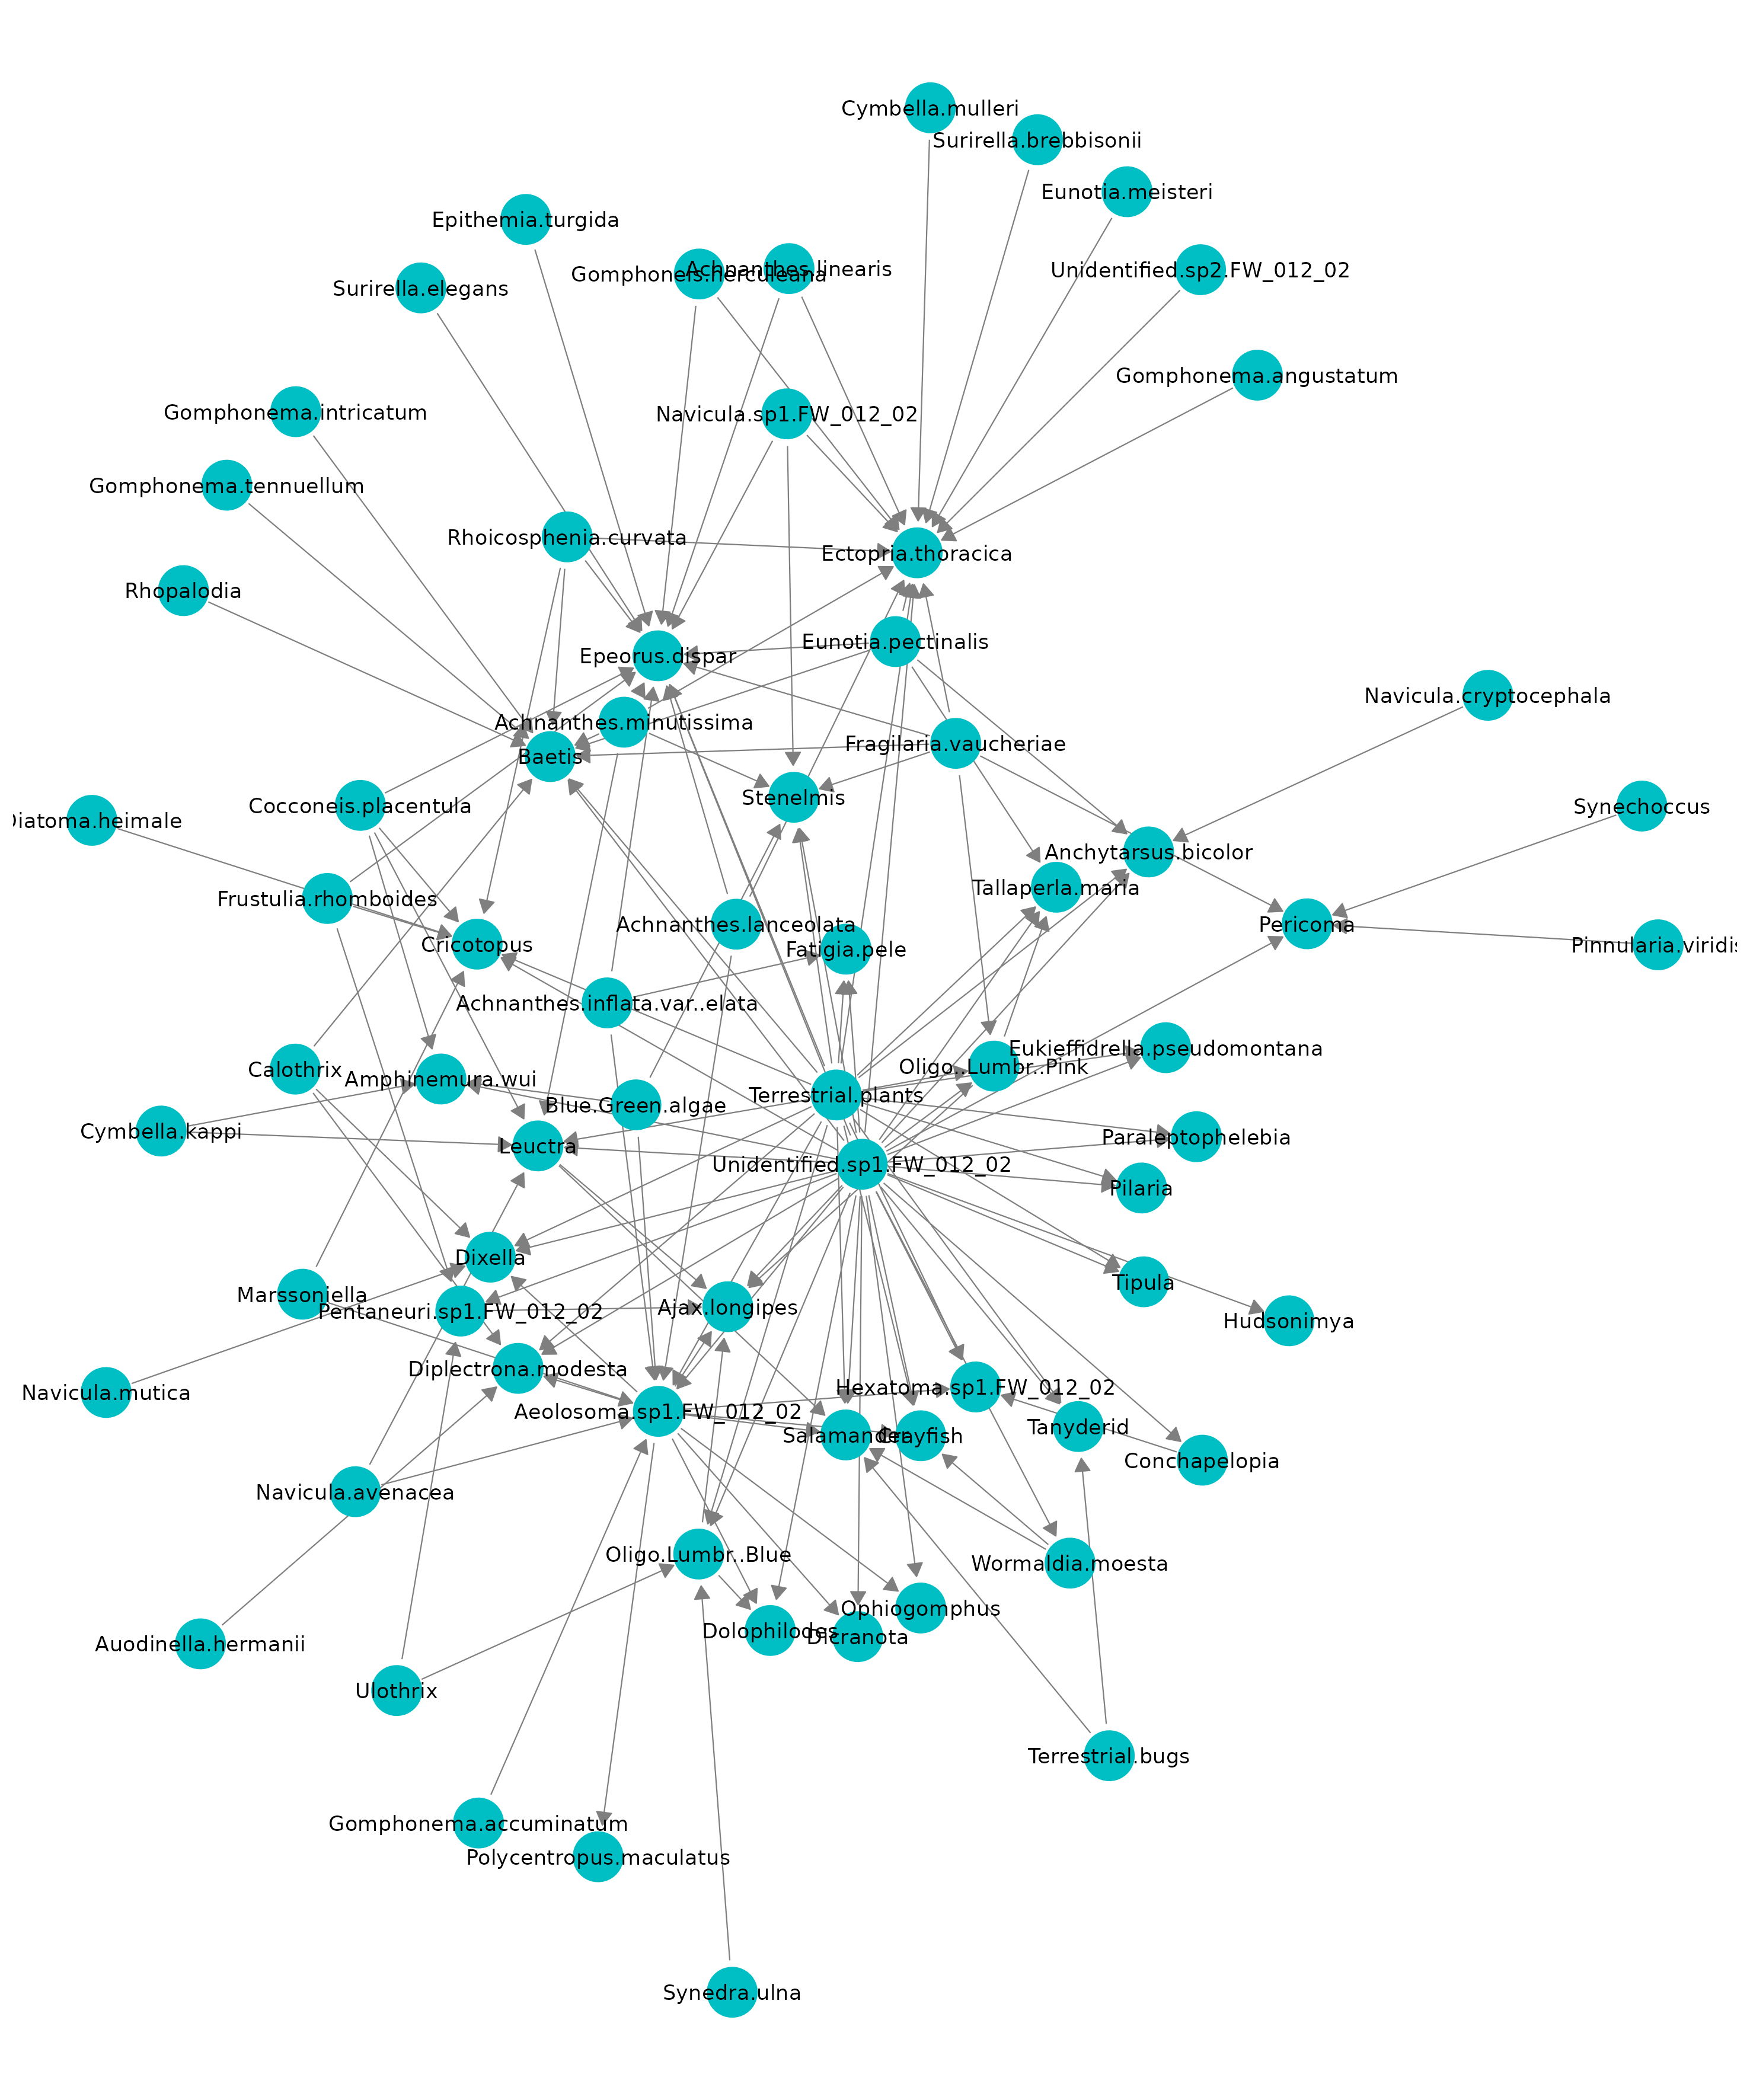
\includegraphics[width=0.45\textwidth]{plots/network_Herlzier(NC)}

}

%====================================================================
\frame{\frametitle{Foodwebs: adjacency matrix}
%====================================================================

 
 
\begin{itemize}
\item $Y = (Y_{ij})_{1 \leq i, j, \leq n}= n \times n$ matrix
\item $Y_{ij}=1$ if $i$ is eaten by $j$, $0$ otherwise
\end{itemize}
 
\begin{columns}
\begin{column}{0.5\textwidth}
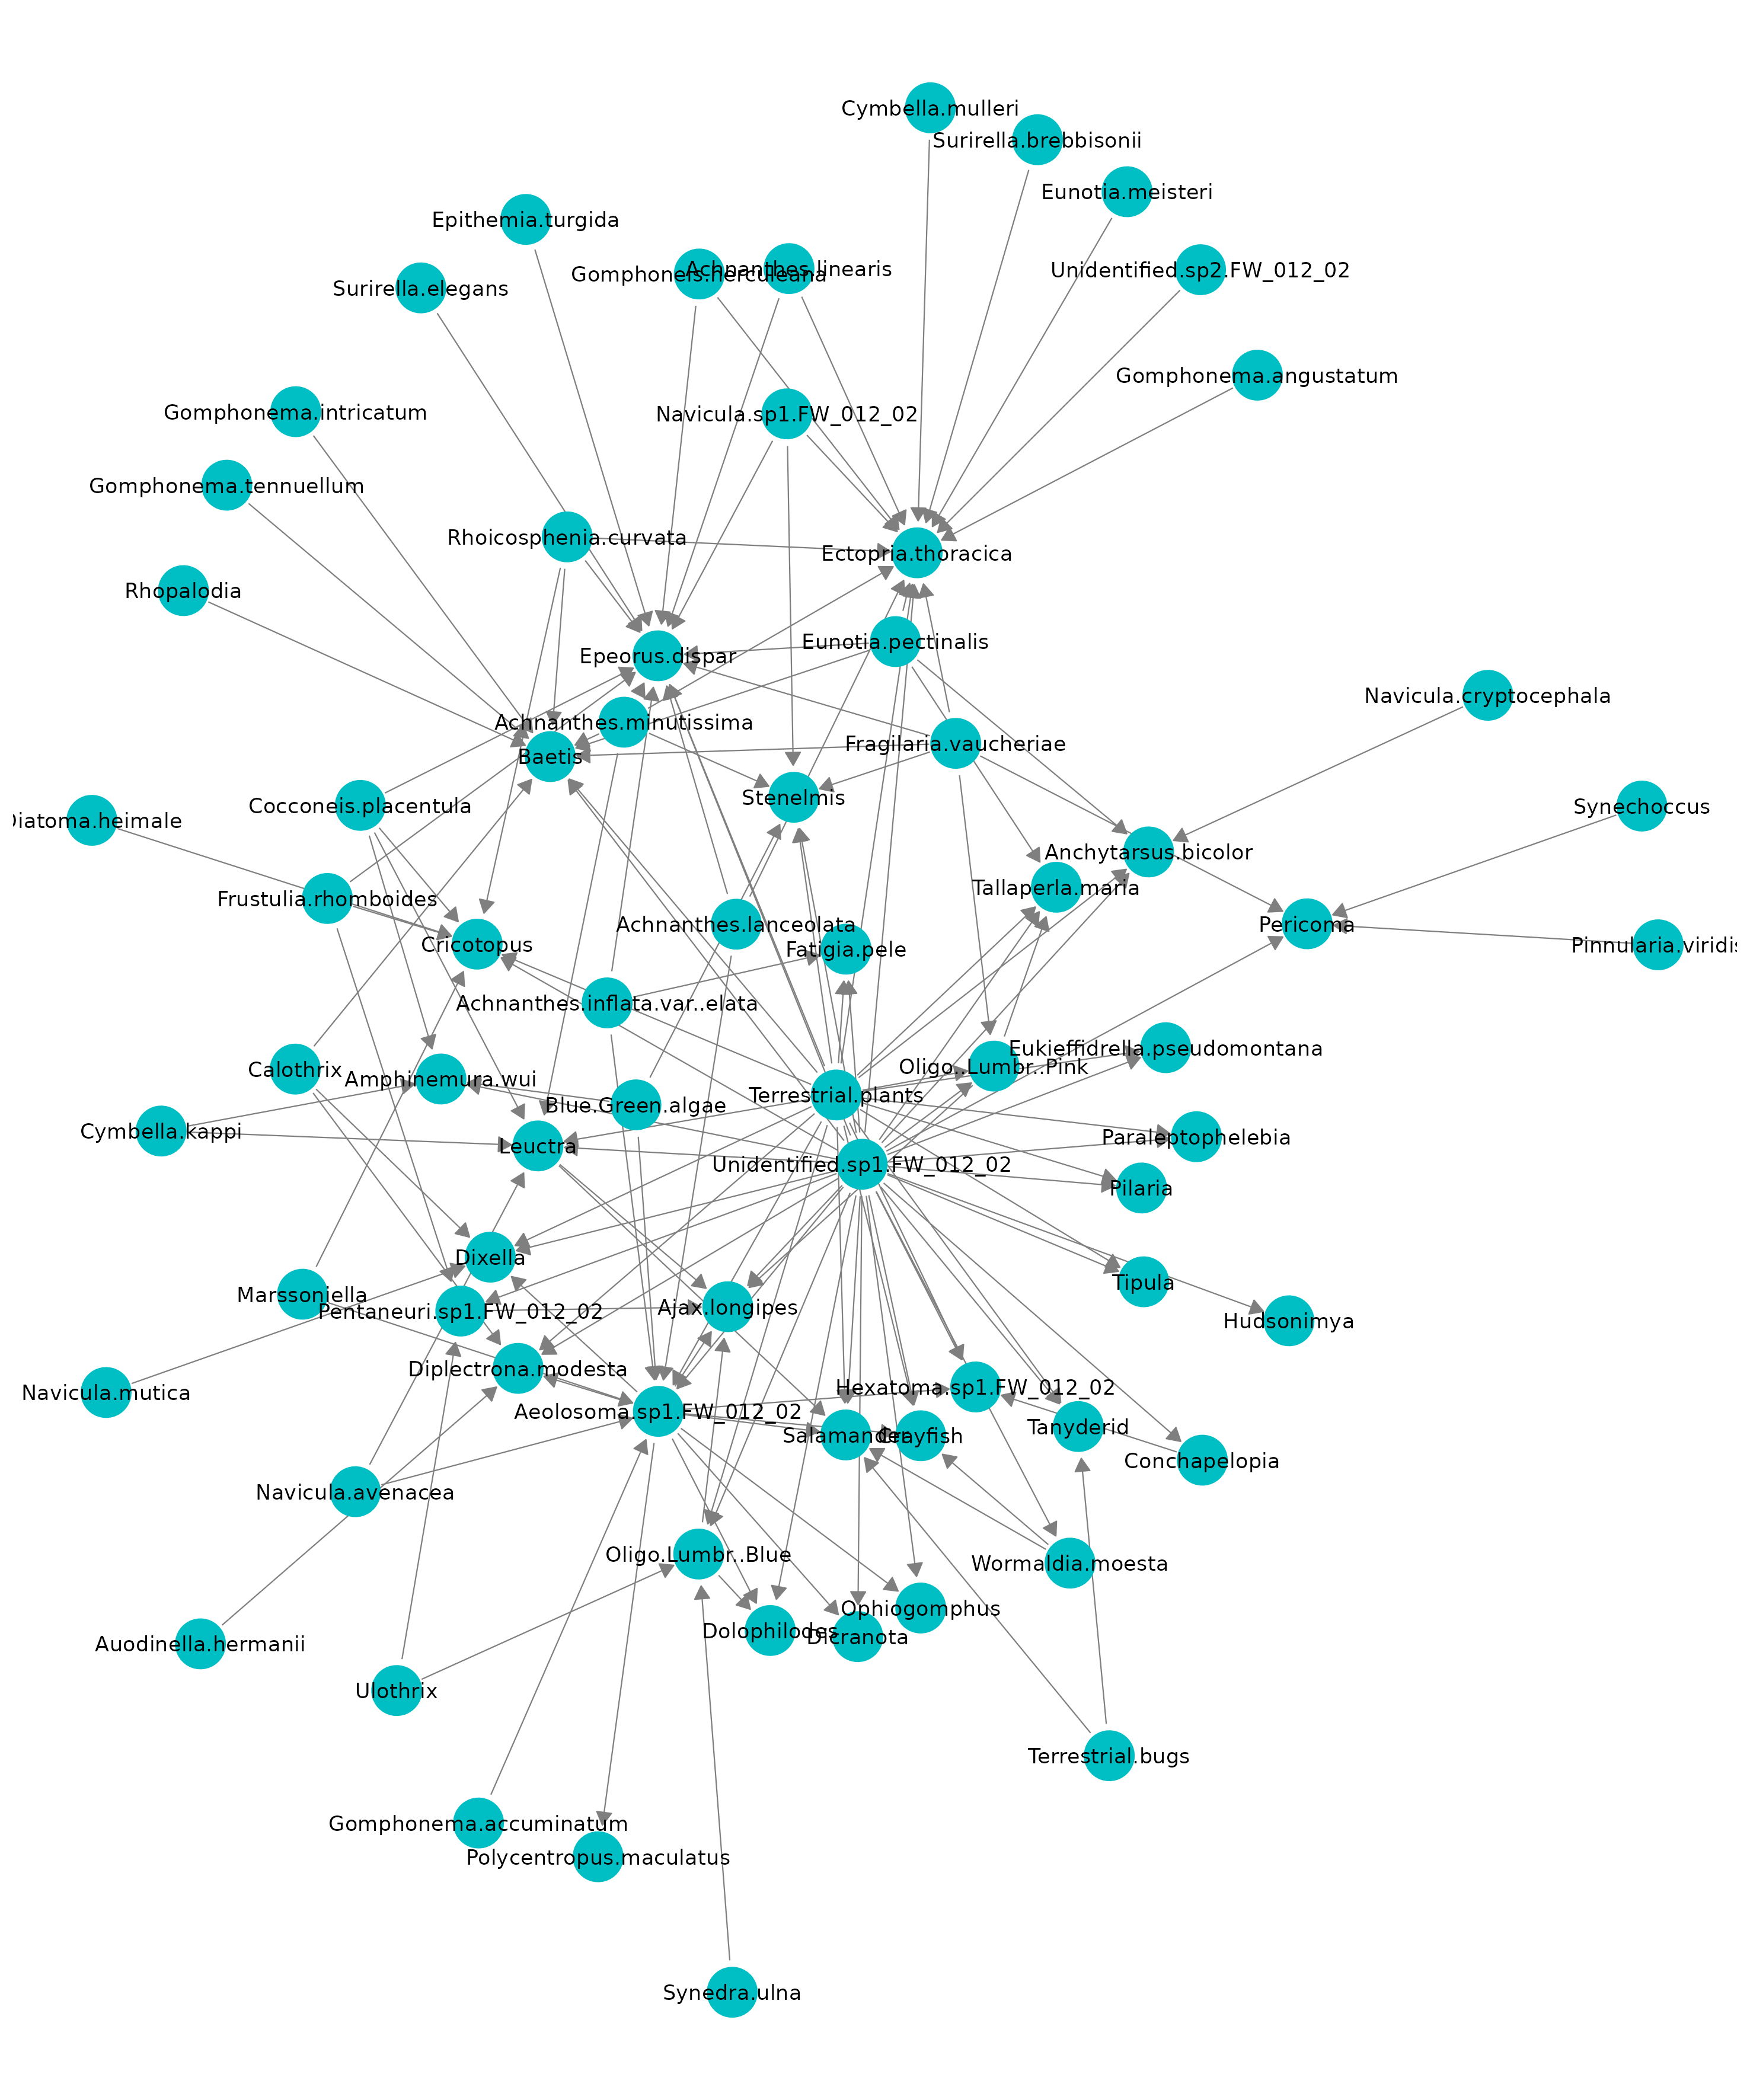
\includegraphics[width=0.9\textwidth]{plots/network_Herlzier(NC)}
\end{column}
\begin{column}{0.5\textwidth}
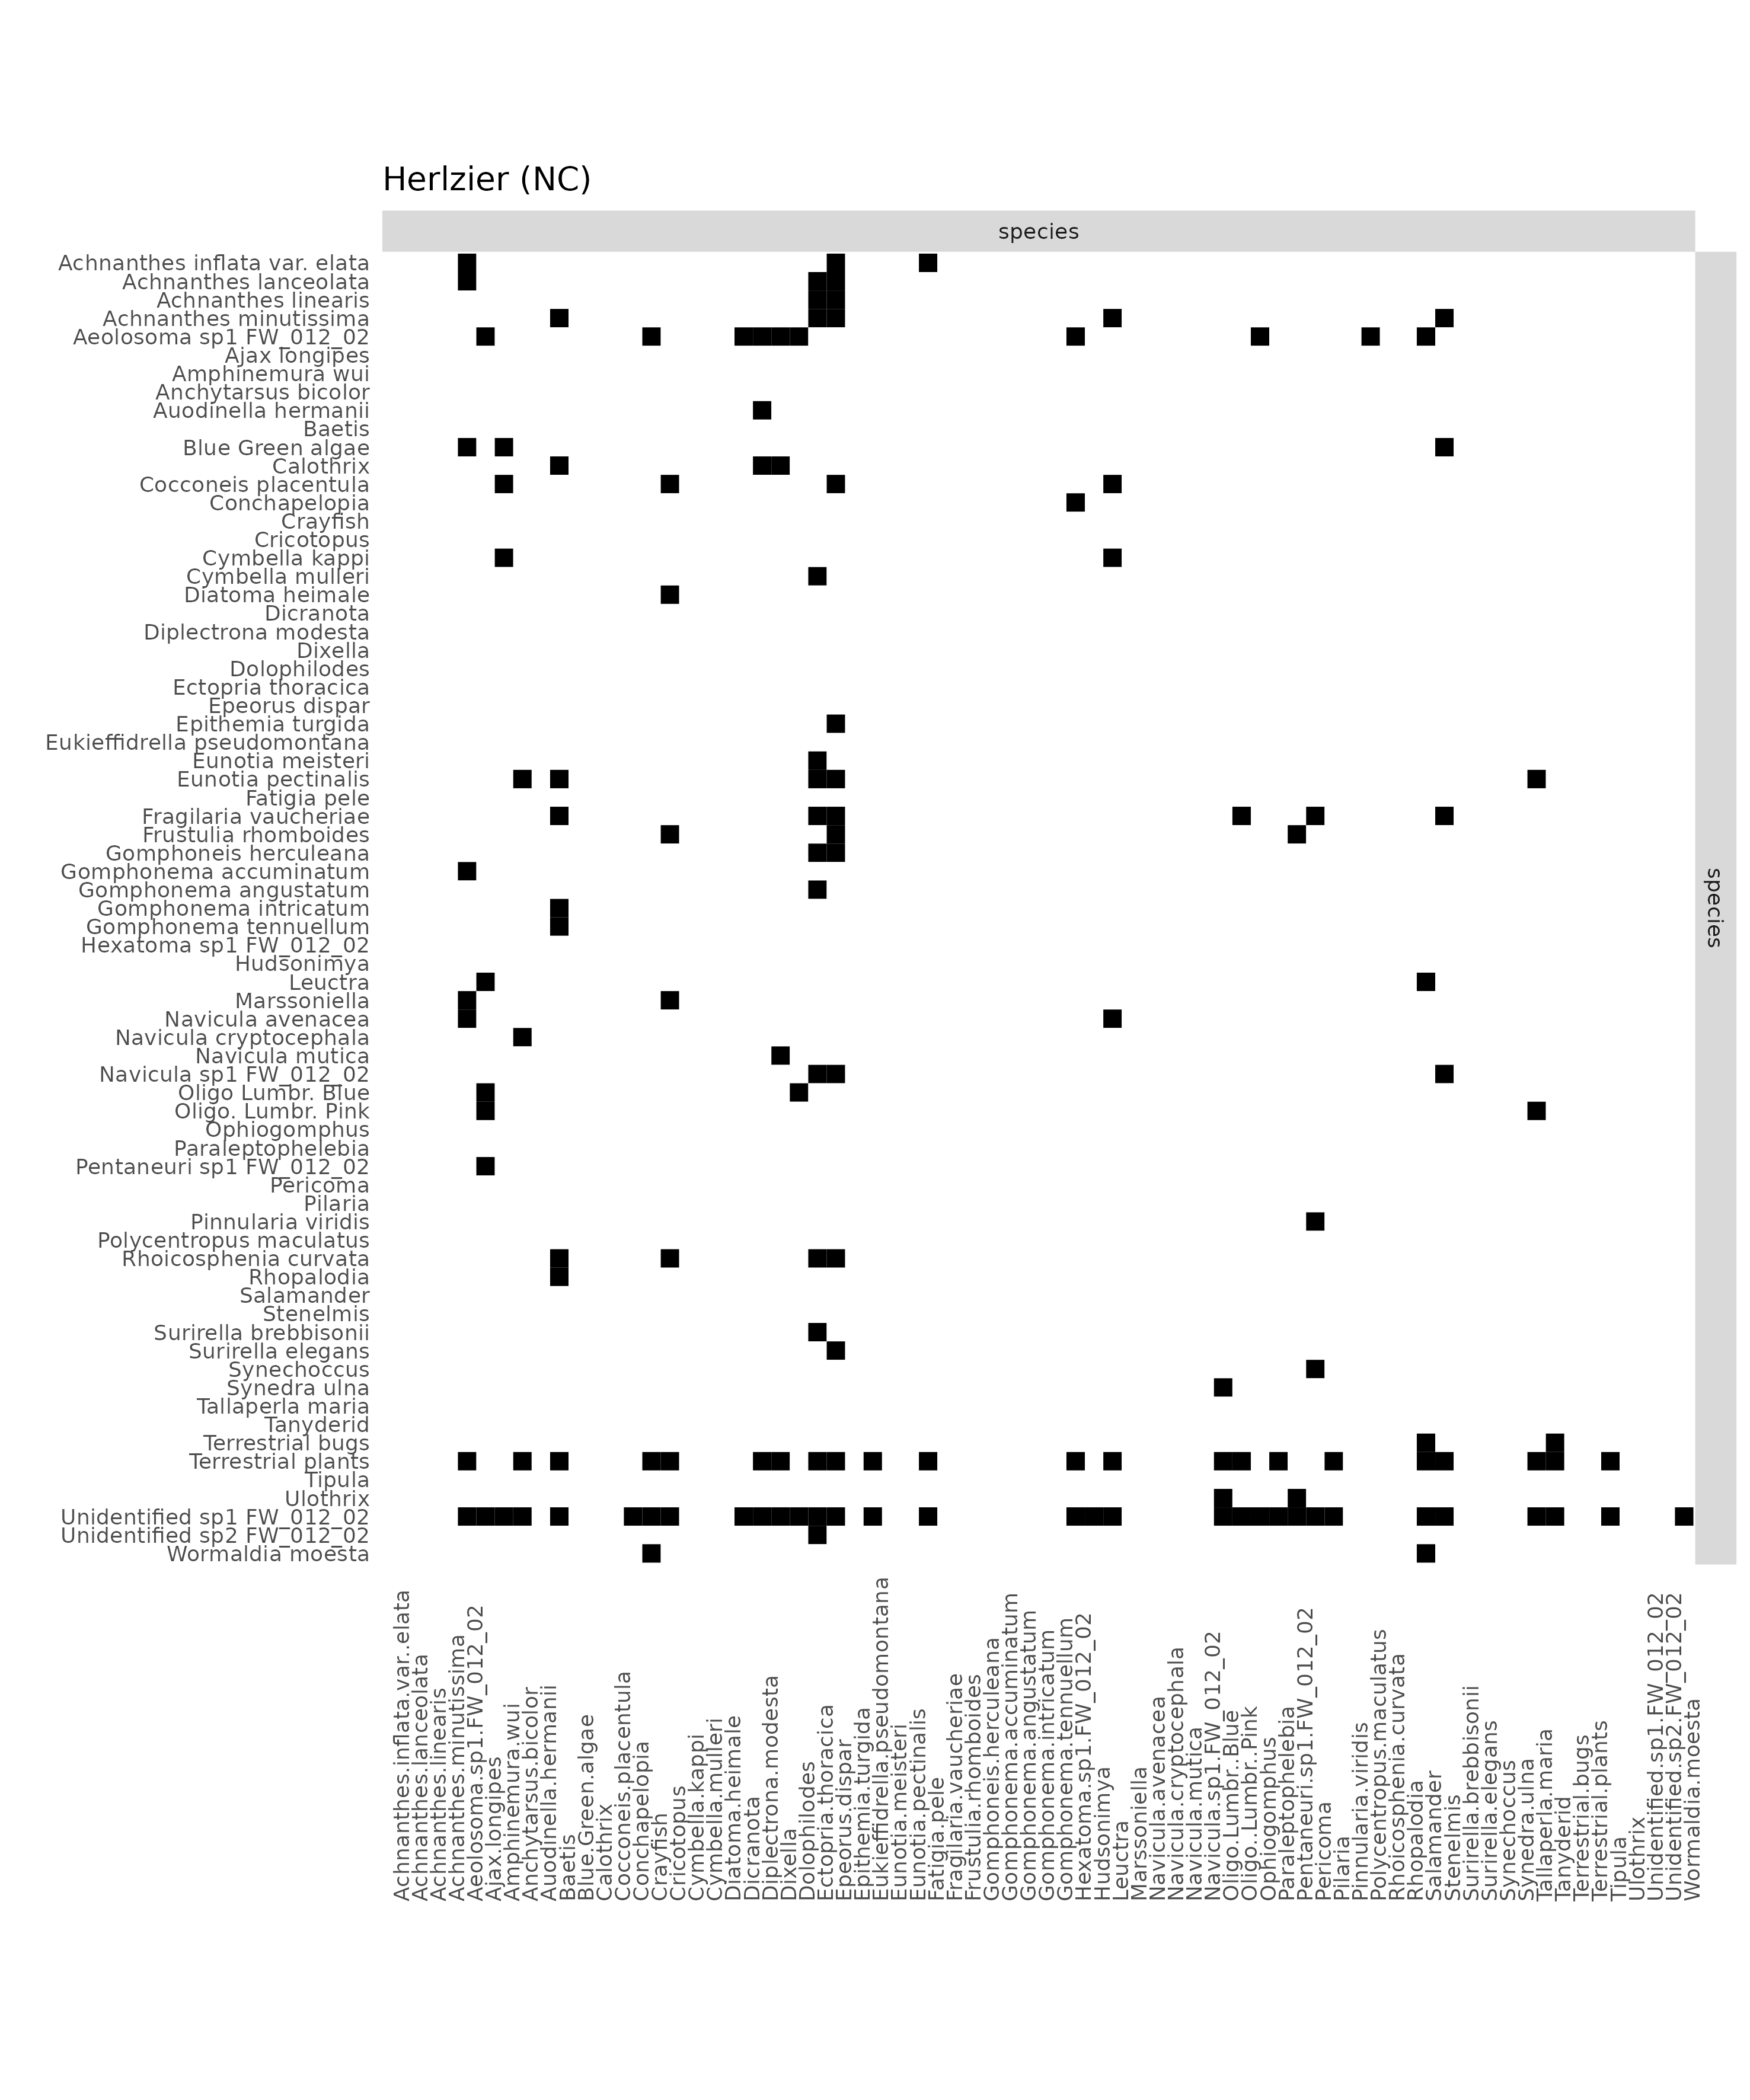
\includegraphics[width=0.8\textwidth]{plots/matrix_Herlzier(NC)}
\end{column}
\end{columns}

\centering

\alert{Directed binary relation : $Y$ non symetric and $0/1$.}


}


%====================================================================
\frame{\frametitle{Parasitism : tree-fungus network} 
%====================================================================
\textcolor{mygreen}{\cite{VPD08}}  Parasitism relation between $n=51$ tree species and $p = 154$ fungus species 

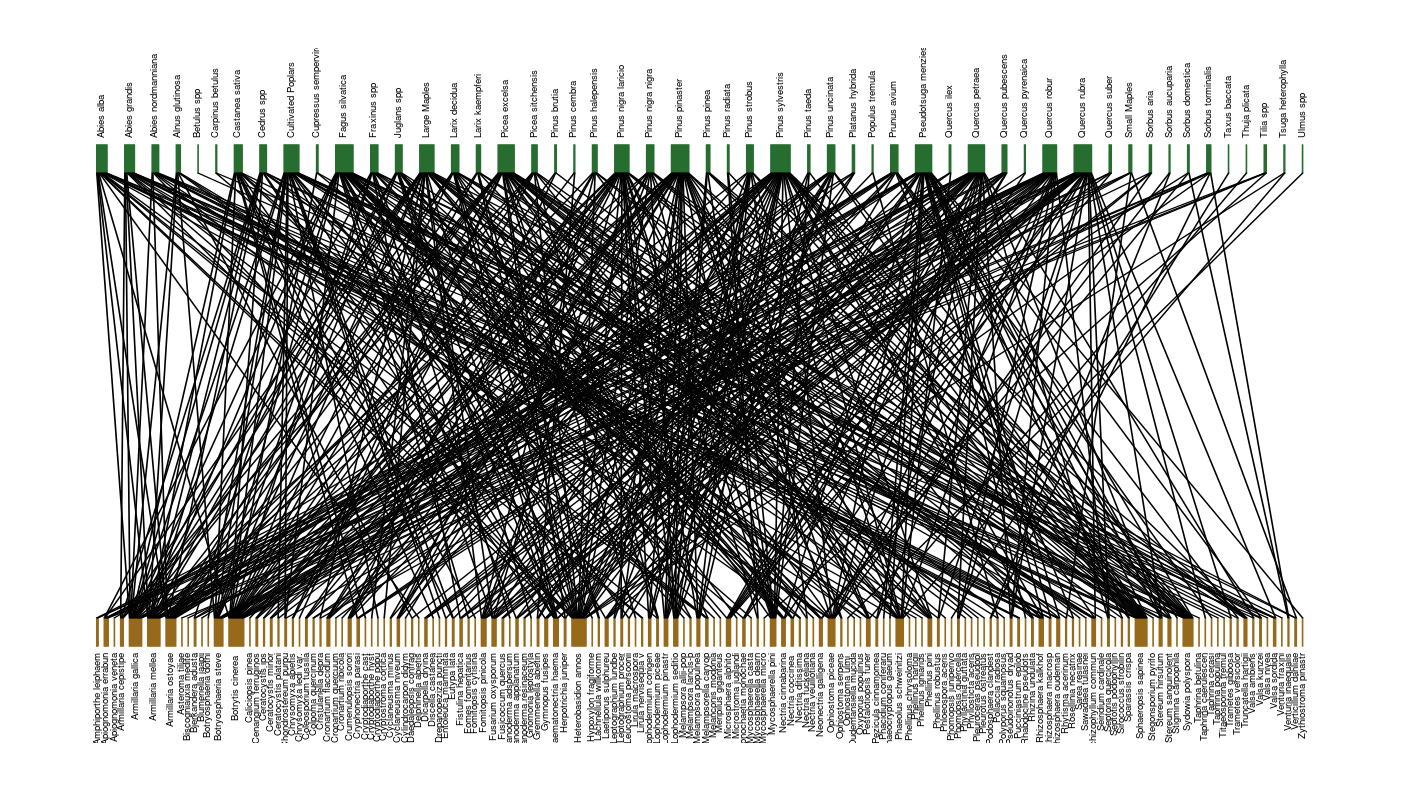
\includegraphics[width=\textwidth]{plots/Tree_fungis_network}

\centering
\alert{Nodes of two types: bipartite network}
}

%====================================================================
\frame{\frametitle{Parasitism : tree-fungus incidence matrix} 
%====================================================================
 

\begin{itemize}
\item $Y = (Y_{ij})_{1 \leq i, j, \leq n}= n \times p$ matrix
\item $Y_{ij}=1$ if tree  $i$ is parasited by fungus  $j$, $0$ otherwise
\end{itemize}
 
\centering
\vspace{-1em} 
% \begin{columns}
% \begin{column}{0.5\textwidth}
% \includegraphics[width=0.9\textwidth]{plots/Tree_fungus_network}
% \end{column}
% \begin{column}{0.5\textwidth}
\includegraphics[width=0.8\textwidth]{plots/Tree_fungis_matrix}
% \end{column}
% \end{columns}

 
\vspace{-3em} 
\alert{Binary bipartite network: $Y$ non square  and $0/1$.}

 

}

%====================================================================
\frame{\frametitle{Parasitism : tree-tree network} 
%====================================================================
\textcolor{mygreen}{\cite{VPD08}}  Number of shared fungus between any pair of the $n=51$ tree species

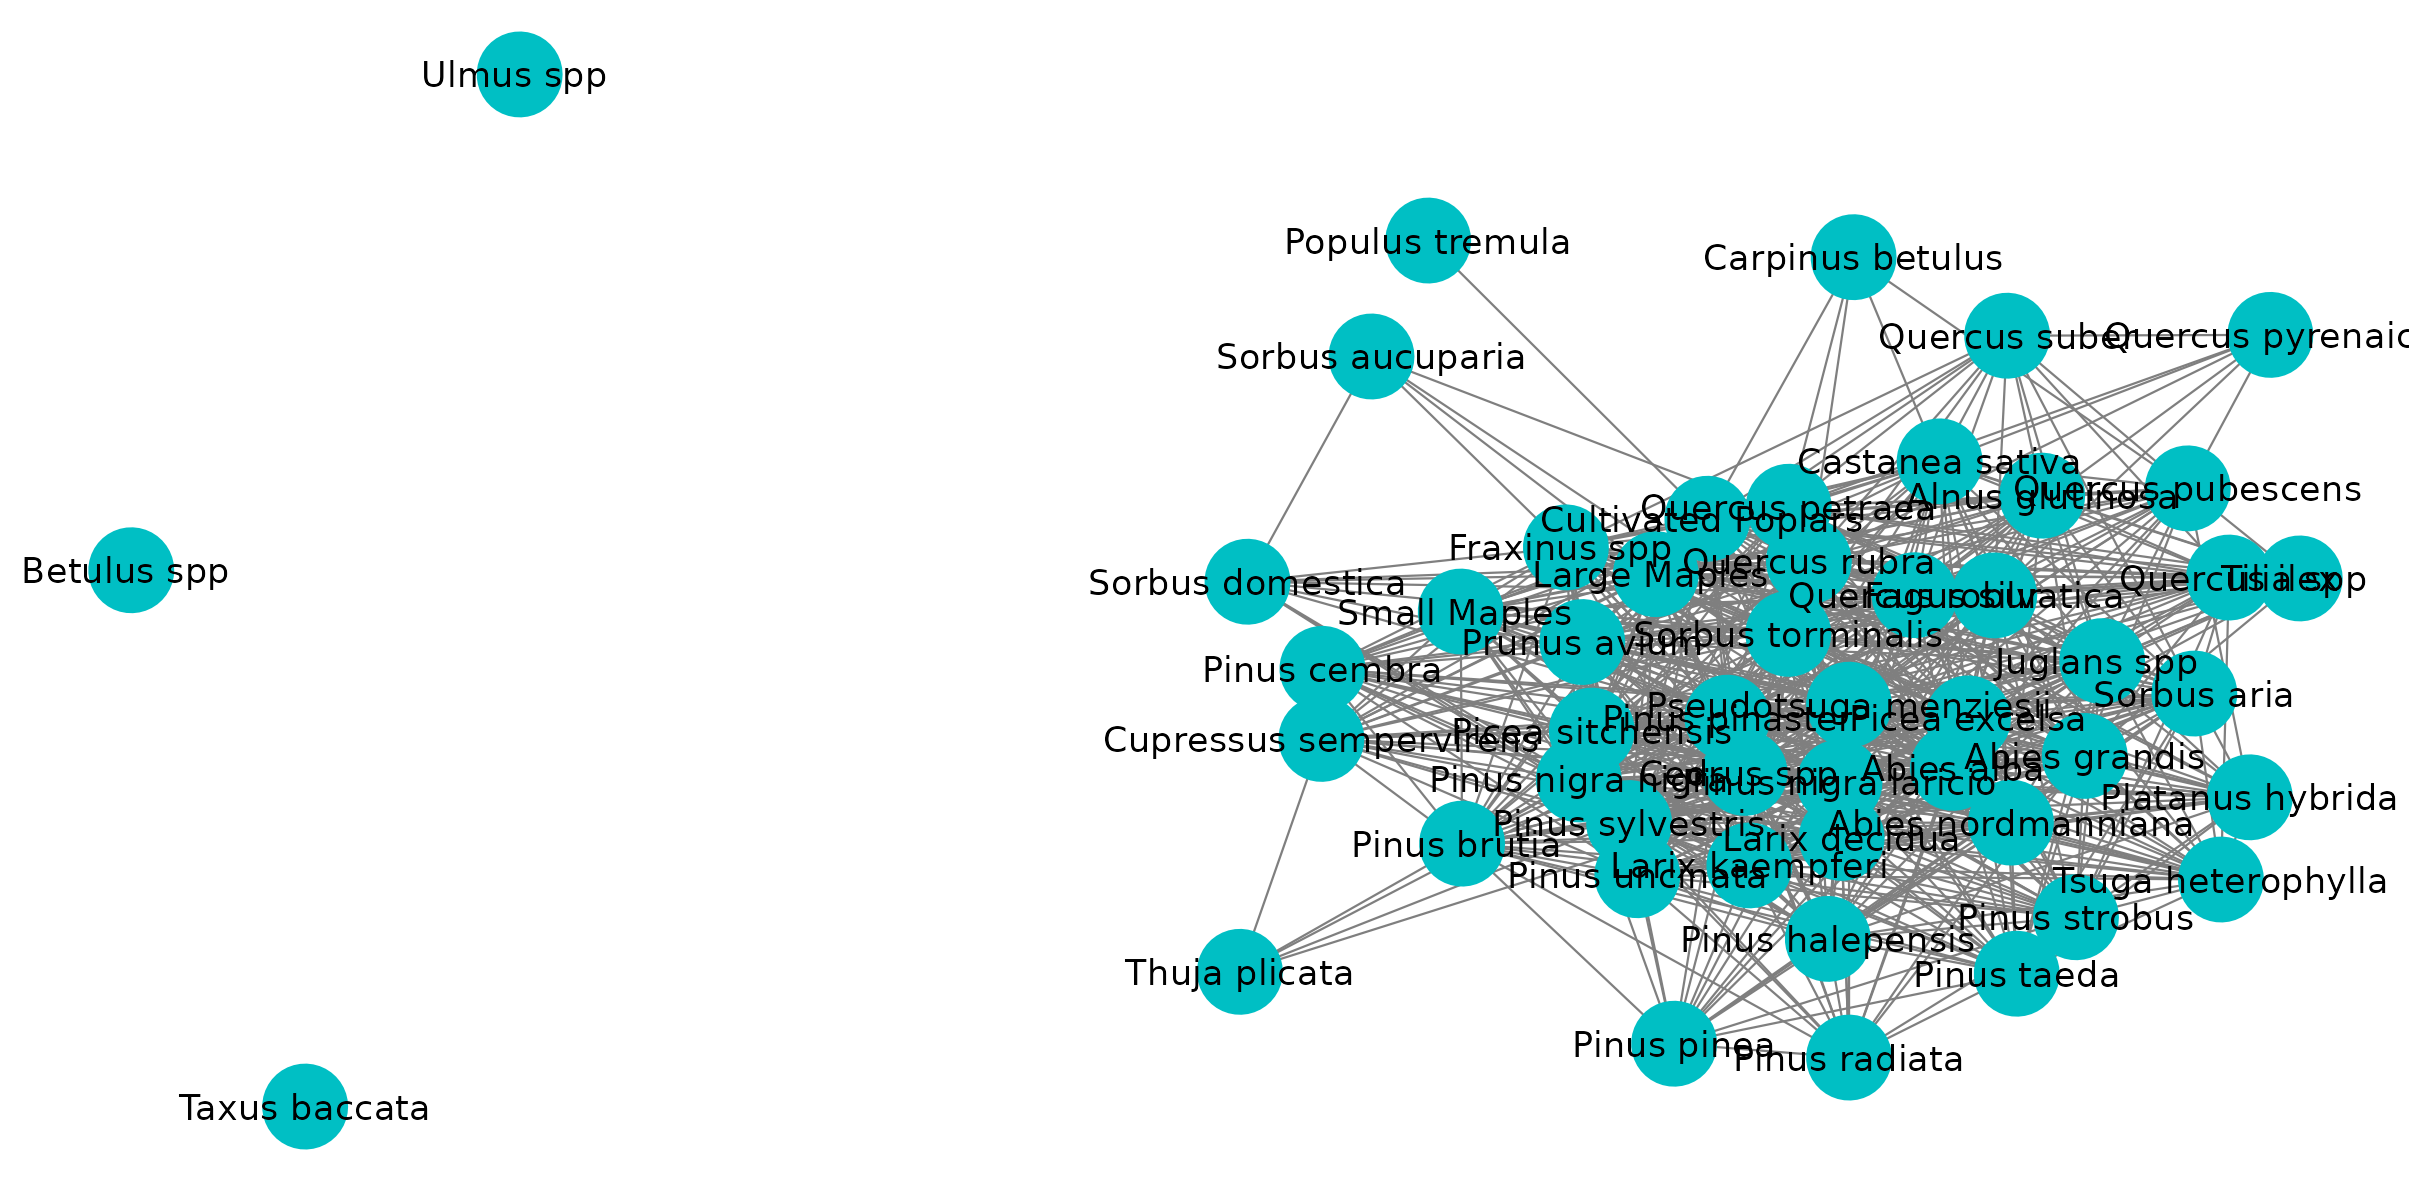
\includegraphics[width=\textwidth]{plots/Tree_network}

}

%====================================================================
\frame{\frametitle{Parasitism : weighted adjacency matrix} 
%====================================================================

 $Y_{ij}$:  number  of shared fungal parasites (fungus  hosted by both species) 
 
\begin{columns}
\begin{column}{0.5\textwidth}
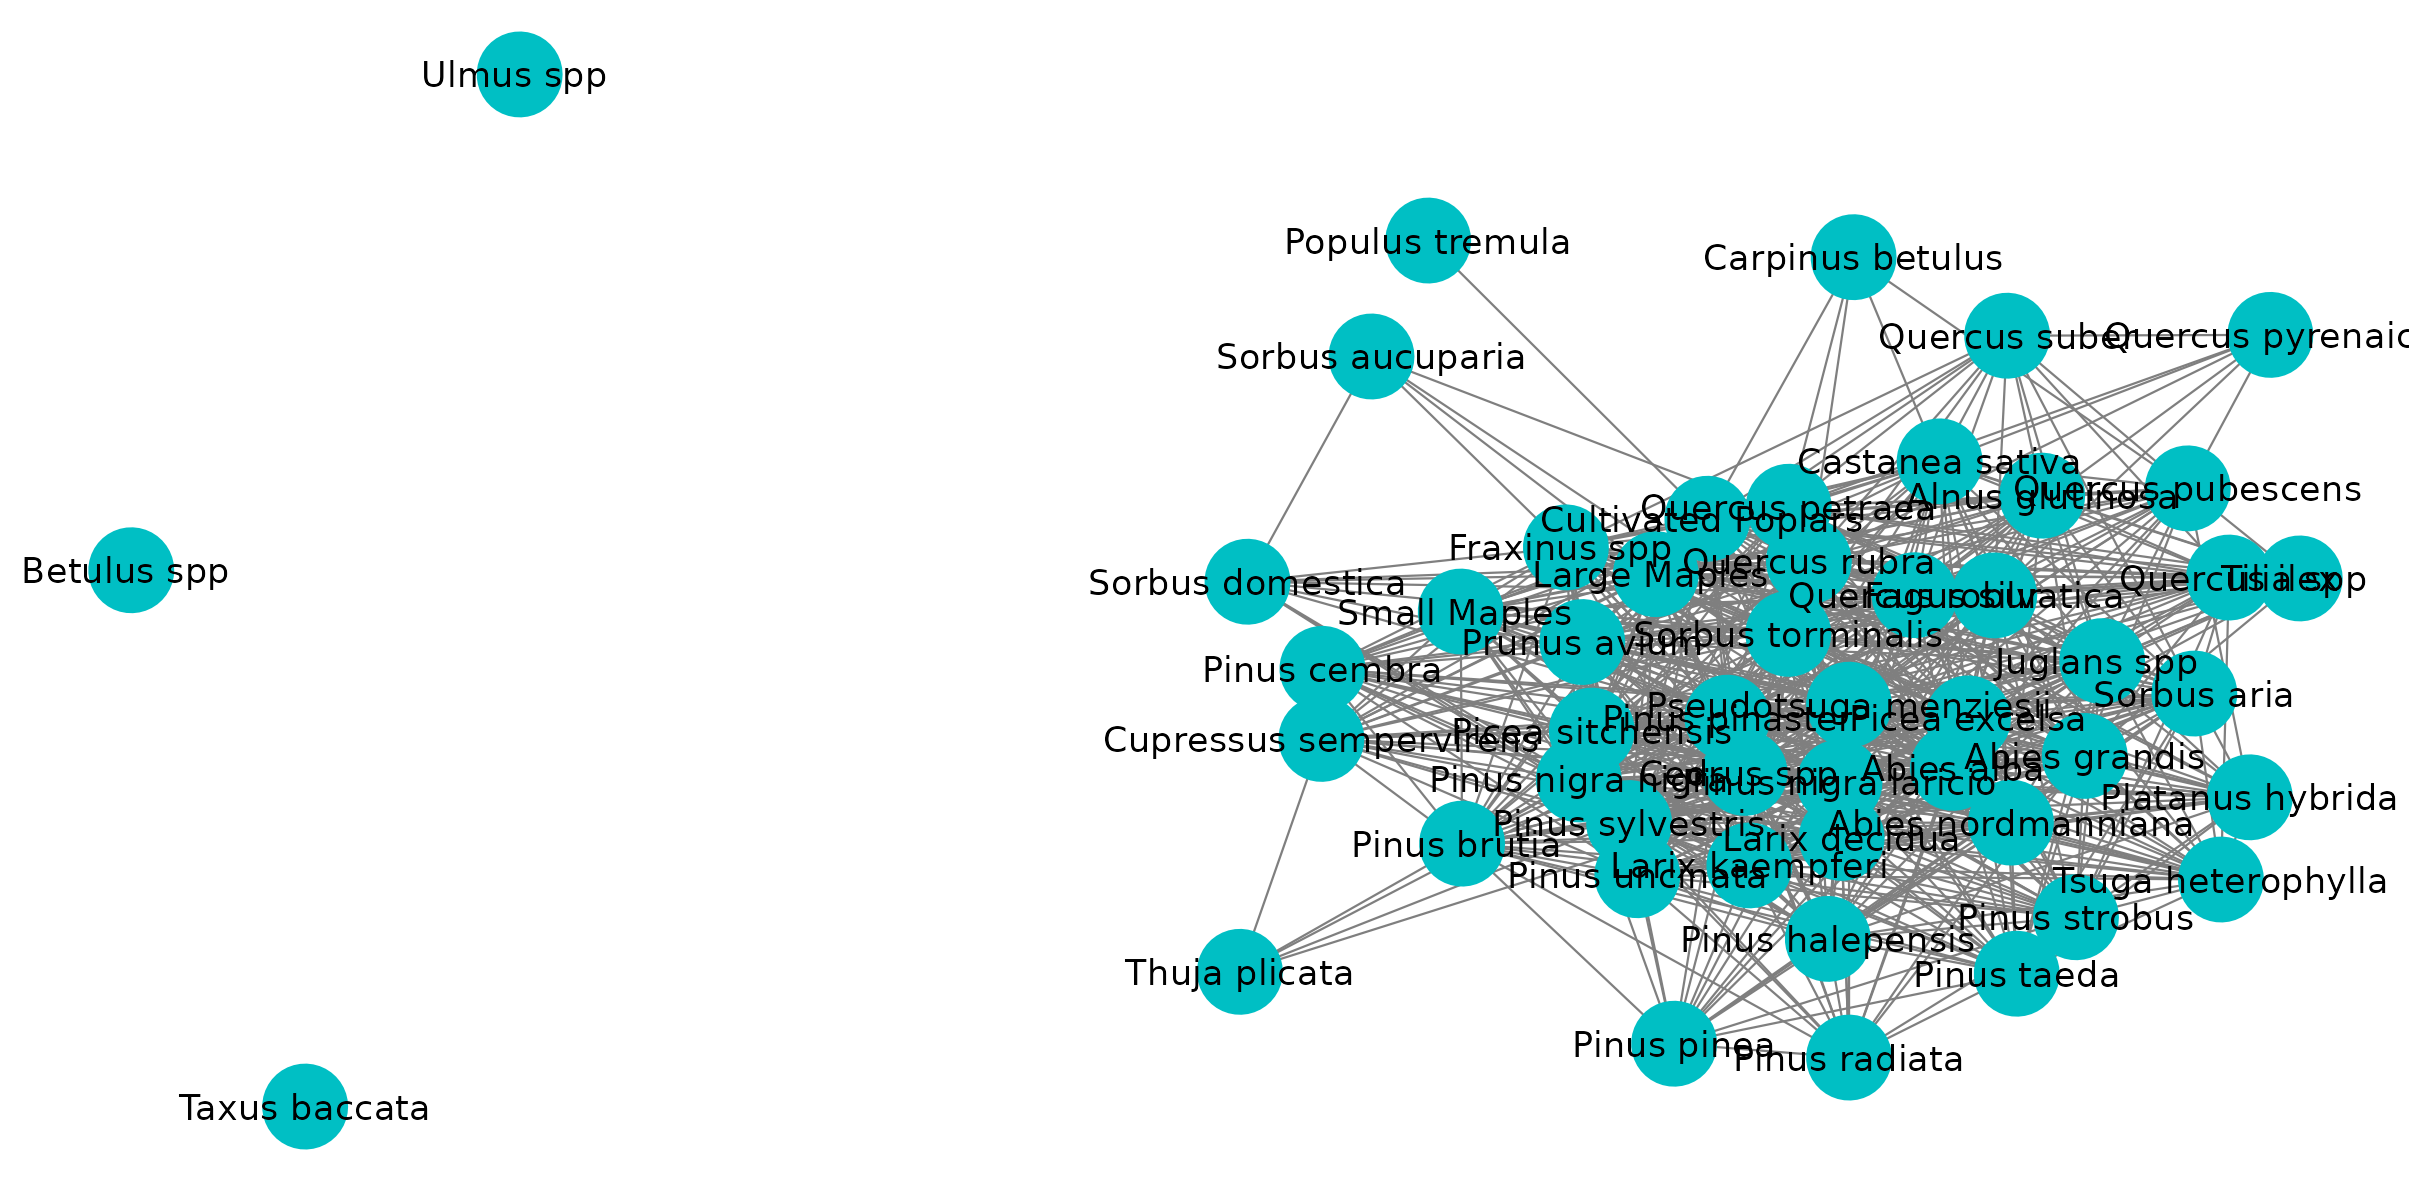
\includegraphics[width=\textwidth]{plots/Tree_network}
\end{column}
\begin{column}{0.5\textwidth}
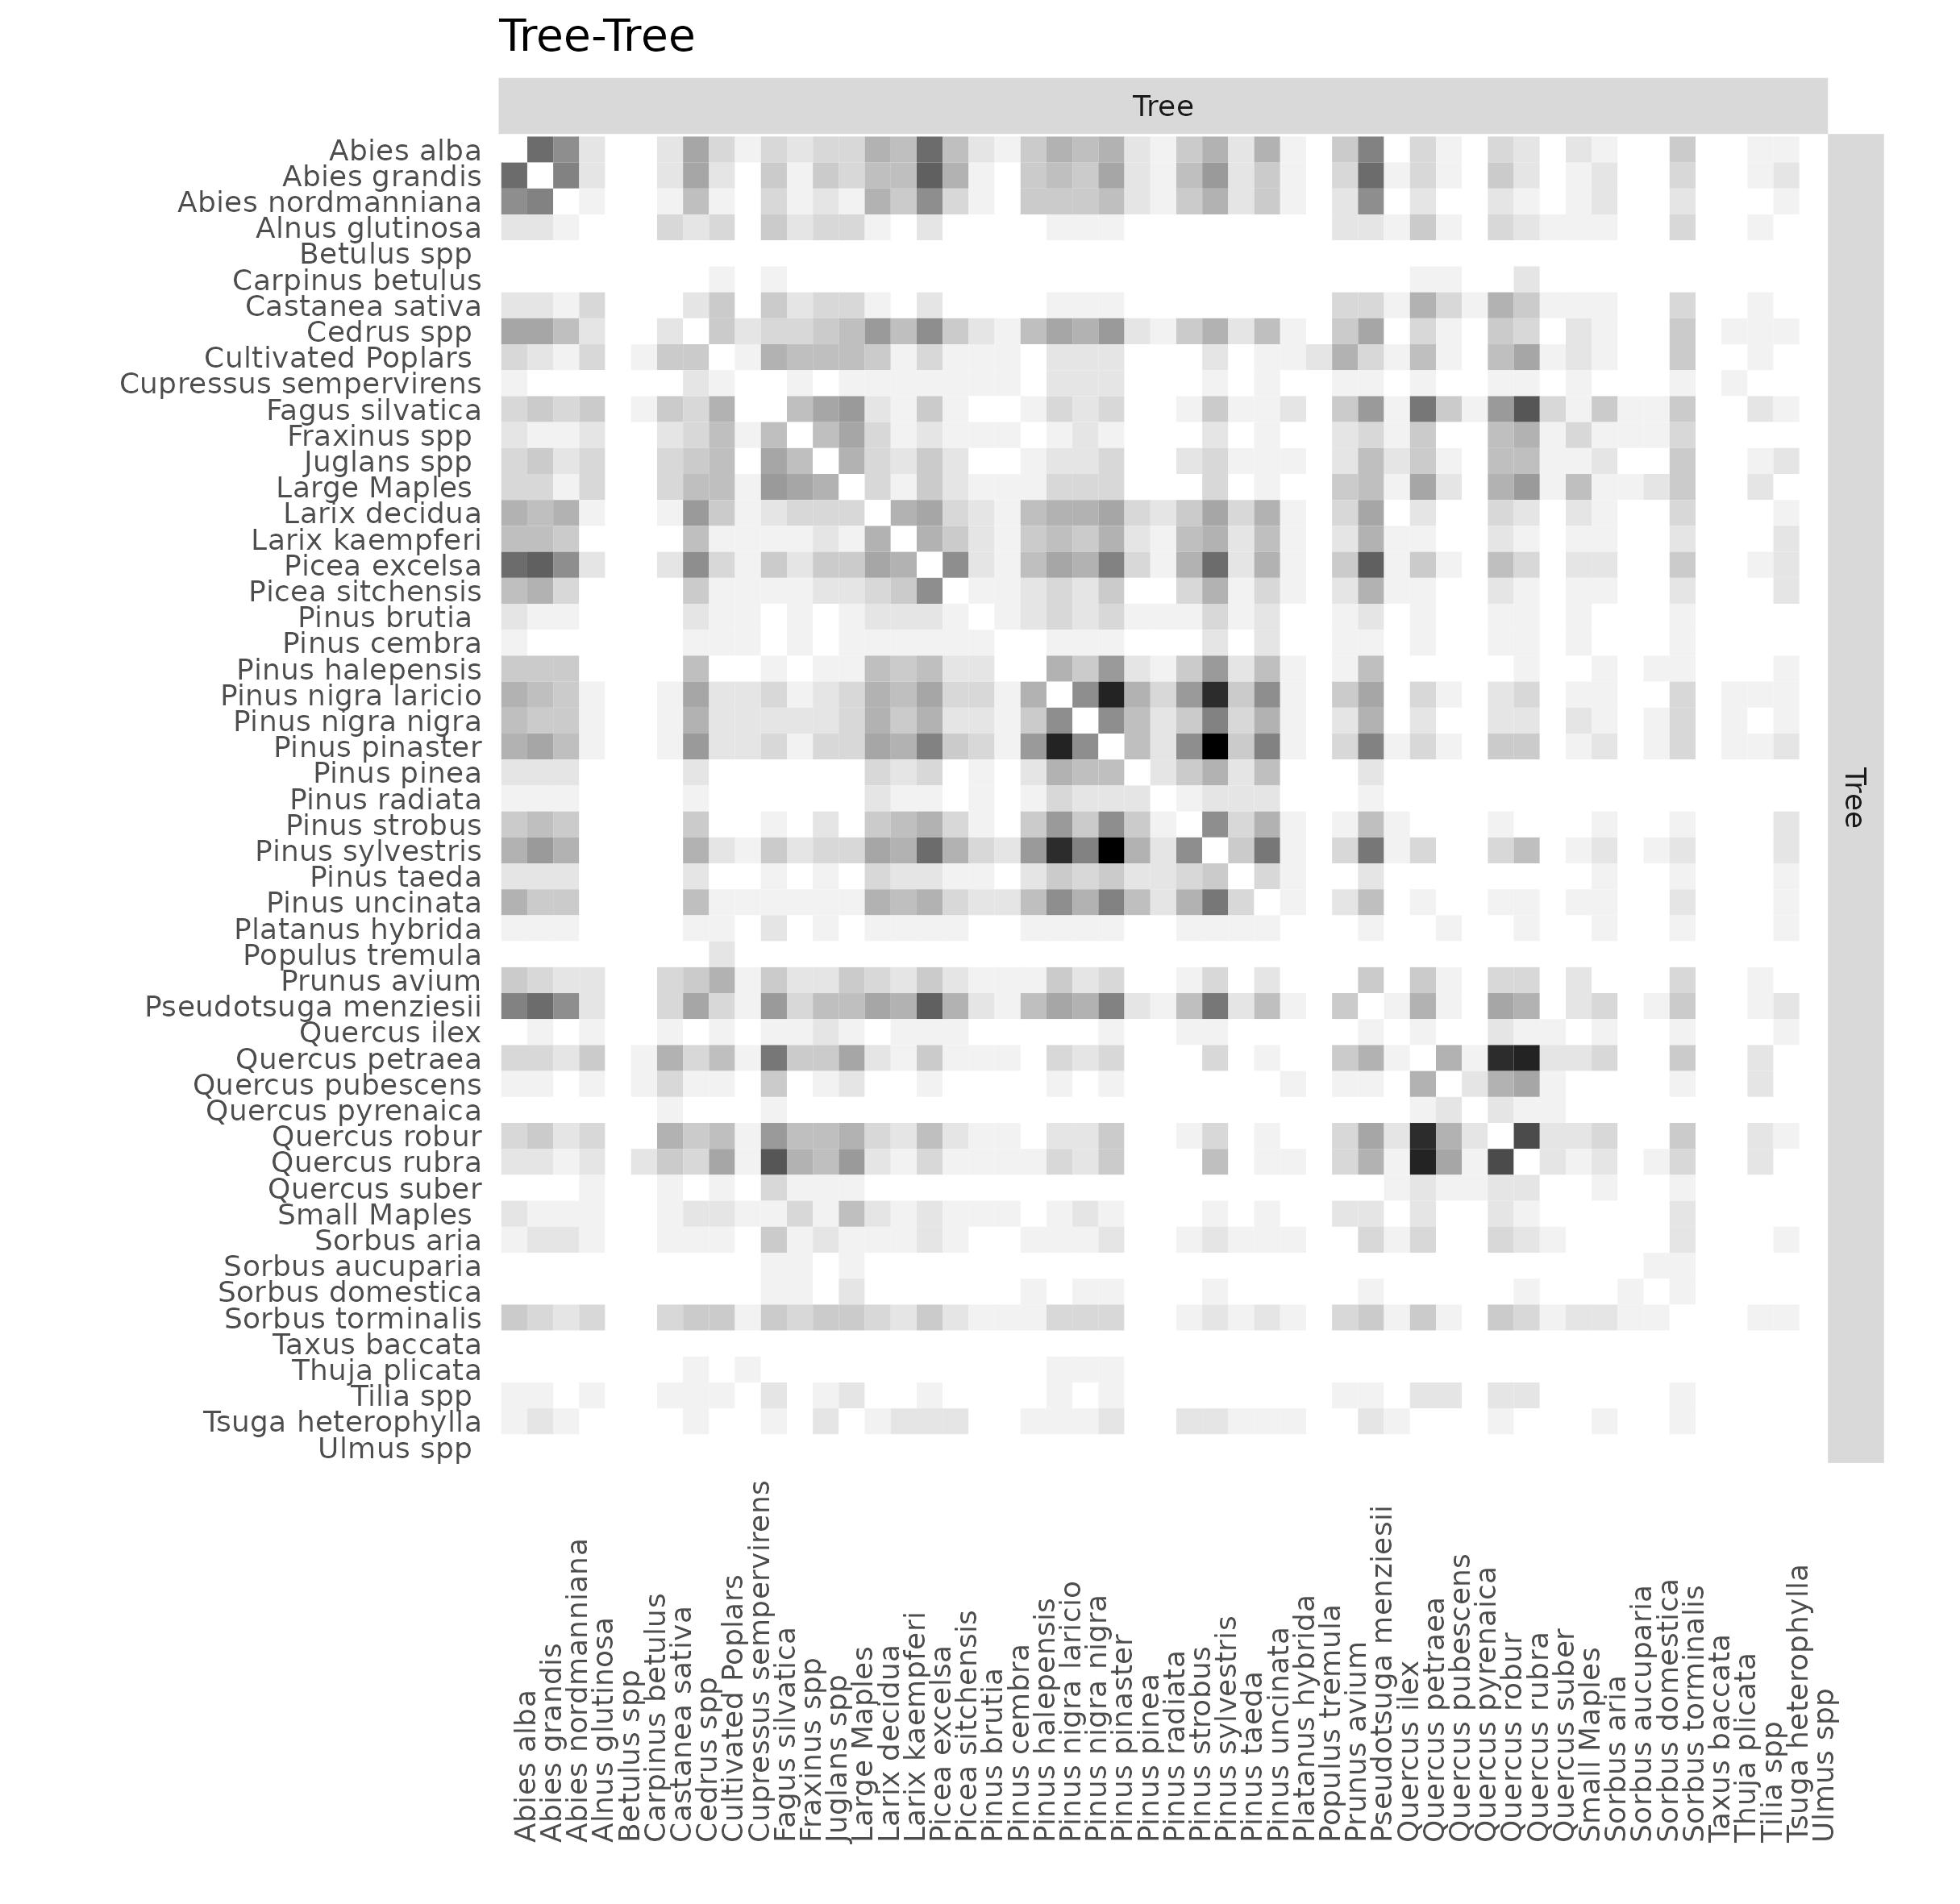
\includegraphics[width= 0.9\textwidth]{plots/Tree_matrix}
\end{column}
 \end{columns}

 
 \centering
\alert{Weighted non-oriented network: $Y$ symetric  and $\in \mathbb{N}$.}
}

 
%====================================================================
\frame{\frametitle{Additional information: covariates on pair of trees} 
%====================================================================

For each pair of tree species, 3 distances were also measured: 

 
\begin{itemize}
\item taxonomic distance ($x^1$) 
\item geographic distance ($x^2$) 
\item genetic distance ($x^3$)
\end{itemize}

 
} 



%====================================================================
\frame[allowframebreaks]{\frametitle{Ecological questions} 
%====================================================================

 \ra \alert{Ecological aim}: caracterize / understand / compare ecosystem organizations. 
%--------------------------------
 
\begin{block}{Foodwebs} 
\begin{itemize}
\item How is organized the network? Can I gather species with similar behavior (trophic levels)? 
\item Do two given species play the same role in the network? 
\end{itemize}
\end{block}
 

\begin{block}{Fungus-tree networks} 
\begin{itemize}
\item Can we find groups of trees and fungi that are preferentially associated? 
\end{itemize}


\end{block}
%--------------------------------
 
\begin{block}{Parasite networks between trees} 
\begin{itemize}
\item Do any of the three distances (genetic, geographic or taxonomic) contributes to shape the number of shared  parasites?  
\item Are the covariates sufficient to explain the interactions? 
\end{itemize}


\end{block}


}




%====================================================================
\begin{frame} \frametitle{Statistical inference: available data}
%====================================================================
 
\begin{center}
 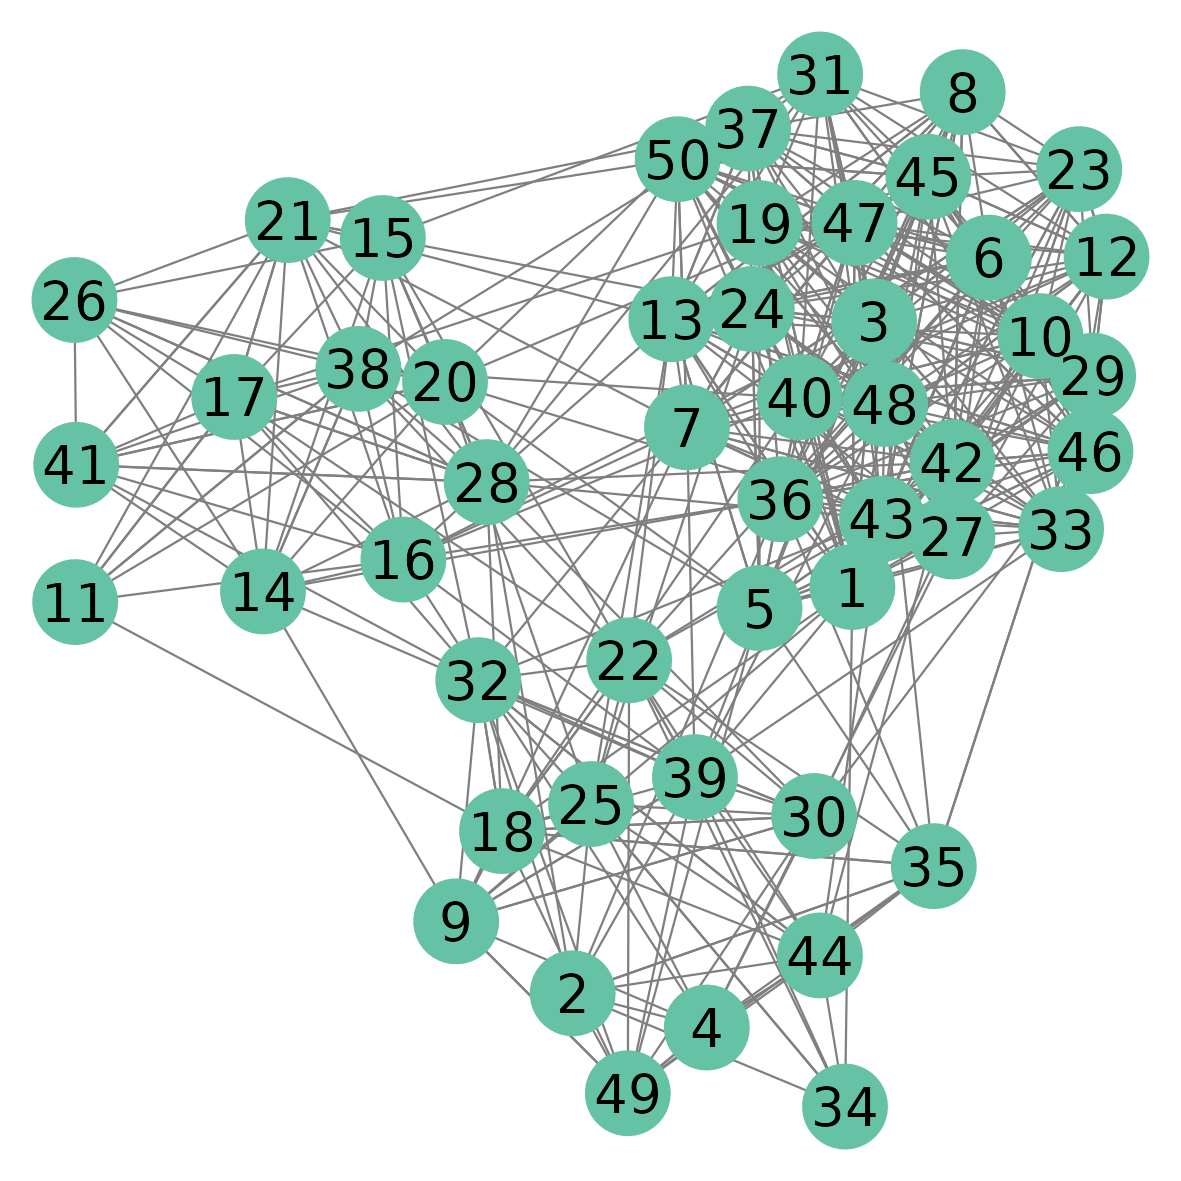
\includegraphics[scale=.45]{plots/network_raw.png}
\end{center}

\begin{itemize}
 \item  the network provided as:
\begin{itemize}
 \item an adjacency matrix (for simple network) or an incidence matrix (for bipartite network),
 \item a list of pair of nodes / dyads which are linked.
\end{itemize}

\item some additional covariates on nodes, dyads which can account for sampling effort.
 \end{itemize}
\end{frame}



%=====================================================
\begin{frame}\frametitle{Statistical inference: goal}
%====================================================================

 
 
\begin{center}
 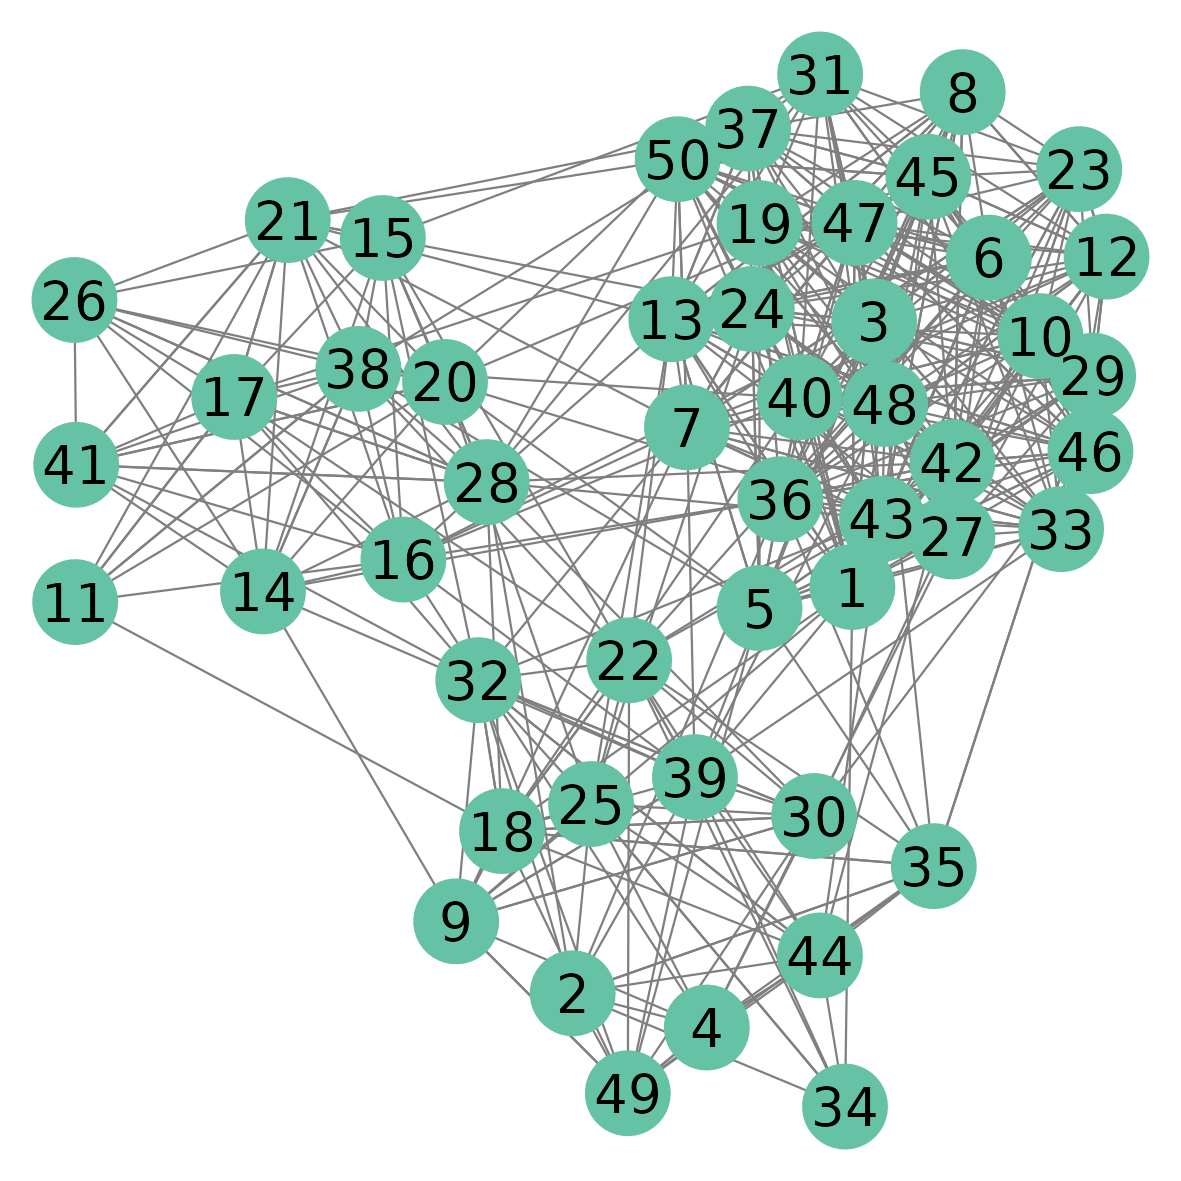
\includegraphics[scale=.45]{plots/network_raw.png}
\end{center}

\begin{itemize}
 \item Unraveling / describing / modeling the network topology. 
 \item Discovering particular structure of interactions between some subsets of nodes.
 \item Understanding node heterogeneity.
 \item Not inferring the network !
 \end{itemize}


\end{frame}




%=====================================================
\section{Descriptive statistics}
%=====================================================

%=====================================================
\begin{frame}\frametitle{Some common features studied on networks}
%=====================================================

\begin{itemize}
\item Description of the network with some numerical indicators calculated on each nodes, or on the complete network
\item Some of them are complexe from a computational point of view: clustering of nodes, finding shortest path from any pair of nodes...   
\item Specific to each domain
  \begin{itemize}
  \item Sociology: R-package \href{https://cran.r-project.org/web/packages/sna/index.html}{sna} 
  \item Ecology: R-package \href{https://cran.r-project.org/web/packages/bipartite/index.html}{bipartite} 
  \item Generalist: R-package \href{https://igraph.org/r/doc/aaa-igraph-package.html}{igraph}
  \item Vizualisation: Rpackage \href{https://briatte.github.io/ggnet/}{ggnet2}
  \end{itemize}
  
\end{itemize}
\end{frame}





%=====================================================
\begin{frame}\frametitle{Degree of nodes}
%=====================================================
Number of connexions for each node $i=  1, \dots, n,$: $\mbox{deg}(i)=  \sum_{i=1}^{n} Y_{ij}$
\begin{columns}
 \begin{column}{0.4 \textwidth}
\begin{center}
 \includegraphics[height=.96 \textwidth,angle  = 90]{plots/Tree_fungis_matrix}
\end{center}
 \end{column}
 \begin{column}{0.7 \textwidth}
\begin{center}
 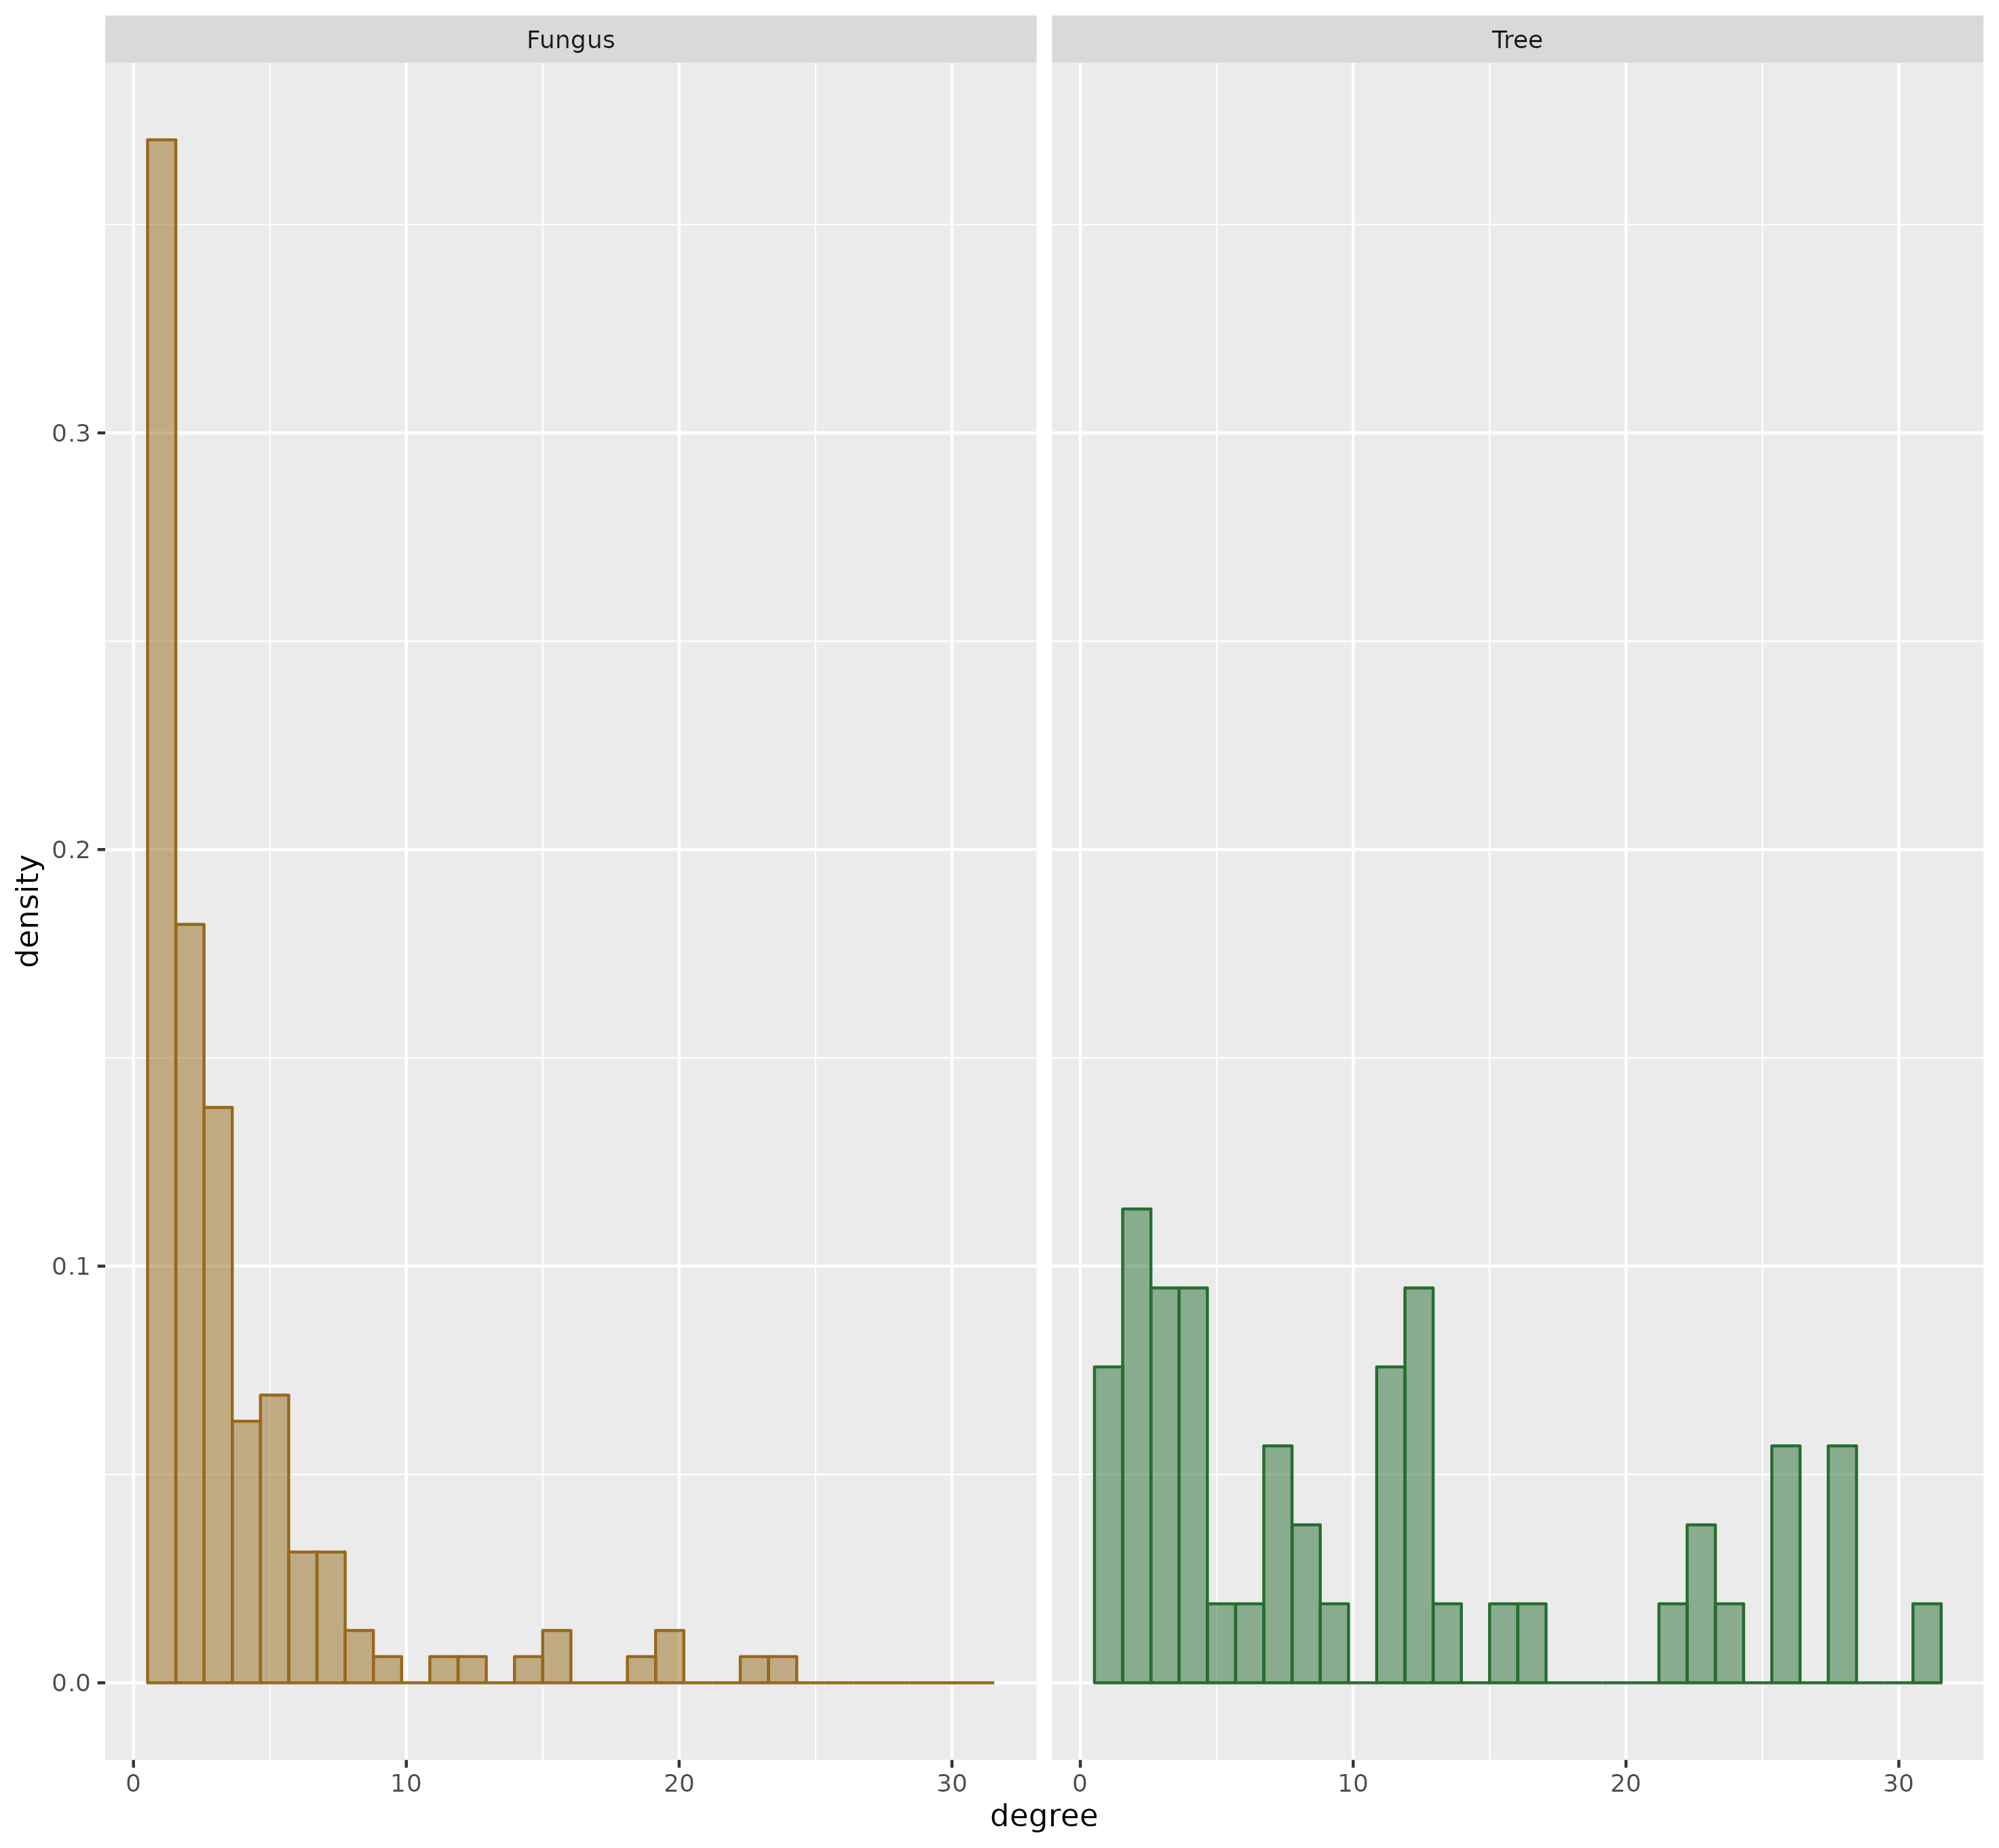
\includegraphics[height=.6 \textheight]{plots/Tree_Fungis_degree.png}
\end{center}
 \end{column}
\end{columns}

\alert{Remarks} 
 Difference of in-degree and out-degree for oriented networks \textcolor{dgreen}{$\bullet$} What if the network is weighted? 



\end{frame}





%=====================================================
\begin{frame}\frametitle{Nestedness, modularity, etc.}
%=====================================================

\begin{itemize}
 \item \alert{Nestedness}: a network is said to be nested when its nodes that have the smallest degree, are connected to nodes with the highest degree \textcolor{mygreen}{\cite{Rodriguez2006}}


\begin{itemize}
\item In other words : specialists are connected to generalist
\item In \href{https://cran.r-project.org/web/packages/bipartite/index.html}{bipartite}: 7 possible ways to measure nestedness
\end{itemize}




\item  \alert{Modularity}: is a measure for a given partition of its tendency of favoring intra-connection over inter-connection.  
\begin{itemize}
\item $\Rightarrow$ Finding the best partition with respect to modularity criterion. 
\textcolor{mygreen}{\cite{clauset2008hierarchical}}
\end{itemize}

\end{itemize}

\bigskip
\centering

All these indicators are \alert{looking for a specific pattern.}
\end{frame}

%%=====================================================
\section{Probabilistic  model}
%=====================================================

%=====================================================
\begin{frame}{Probabilistic approach}
%=====================================================
\begin{itemize}
\item 
\alert{Context}: our   matrix $Y$ is the realization of a stochastic process.
\item 
\alert{Aim}: Propose a  stochastic process is able to mimic heterogeneity in the connections.  
\item \alert{Advantage}: benefit from the statistical tools (tests,  model selection, etc...)  
\end{itemize}


\end{frame}

%=====================================================
\begin{frame}\frametitle{A first random graph model for network}
%=====================================================
\textcolor{mygreen}{Erd\H{o}s-Rényi (1959)} Model for $n$ nodes 

$$\forall 1\le i,j\le n,\quad Y_{ij}\overset{i.i.d.}{\sim} \mathcal{B}\mbox{ern} (p),$$
where  $p\in[0,1]$ is the  probability for a link to exist. 

\vspace{1em}

\alert{Consequence} $$\mbox{deg}(i) \sim_{i.i.d} \mathcal{B}\mbox{in}(n,p)$$

\end{frame}

%=====================================================
\begin{frame}\frametitle{Confrontation to a real network}
%=====================================================
\begin{columns}
\begin{column}{0.5\textwidth}
\centering
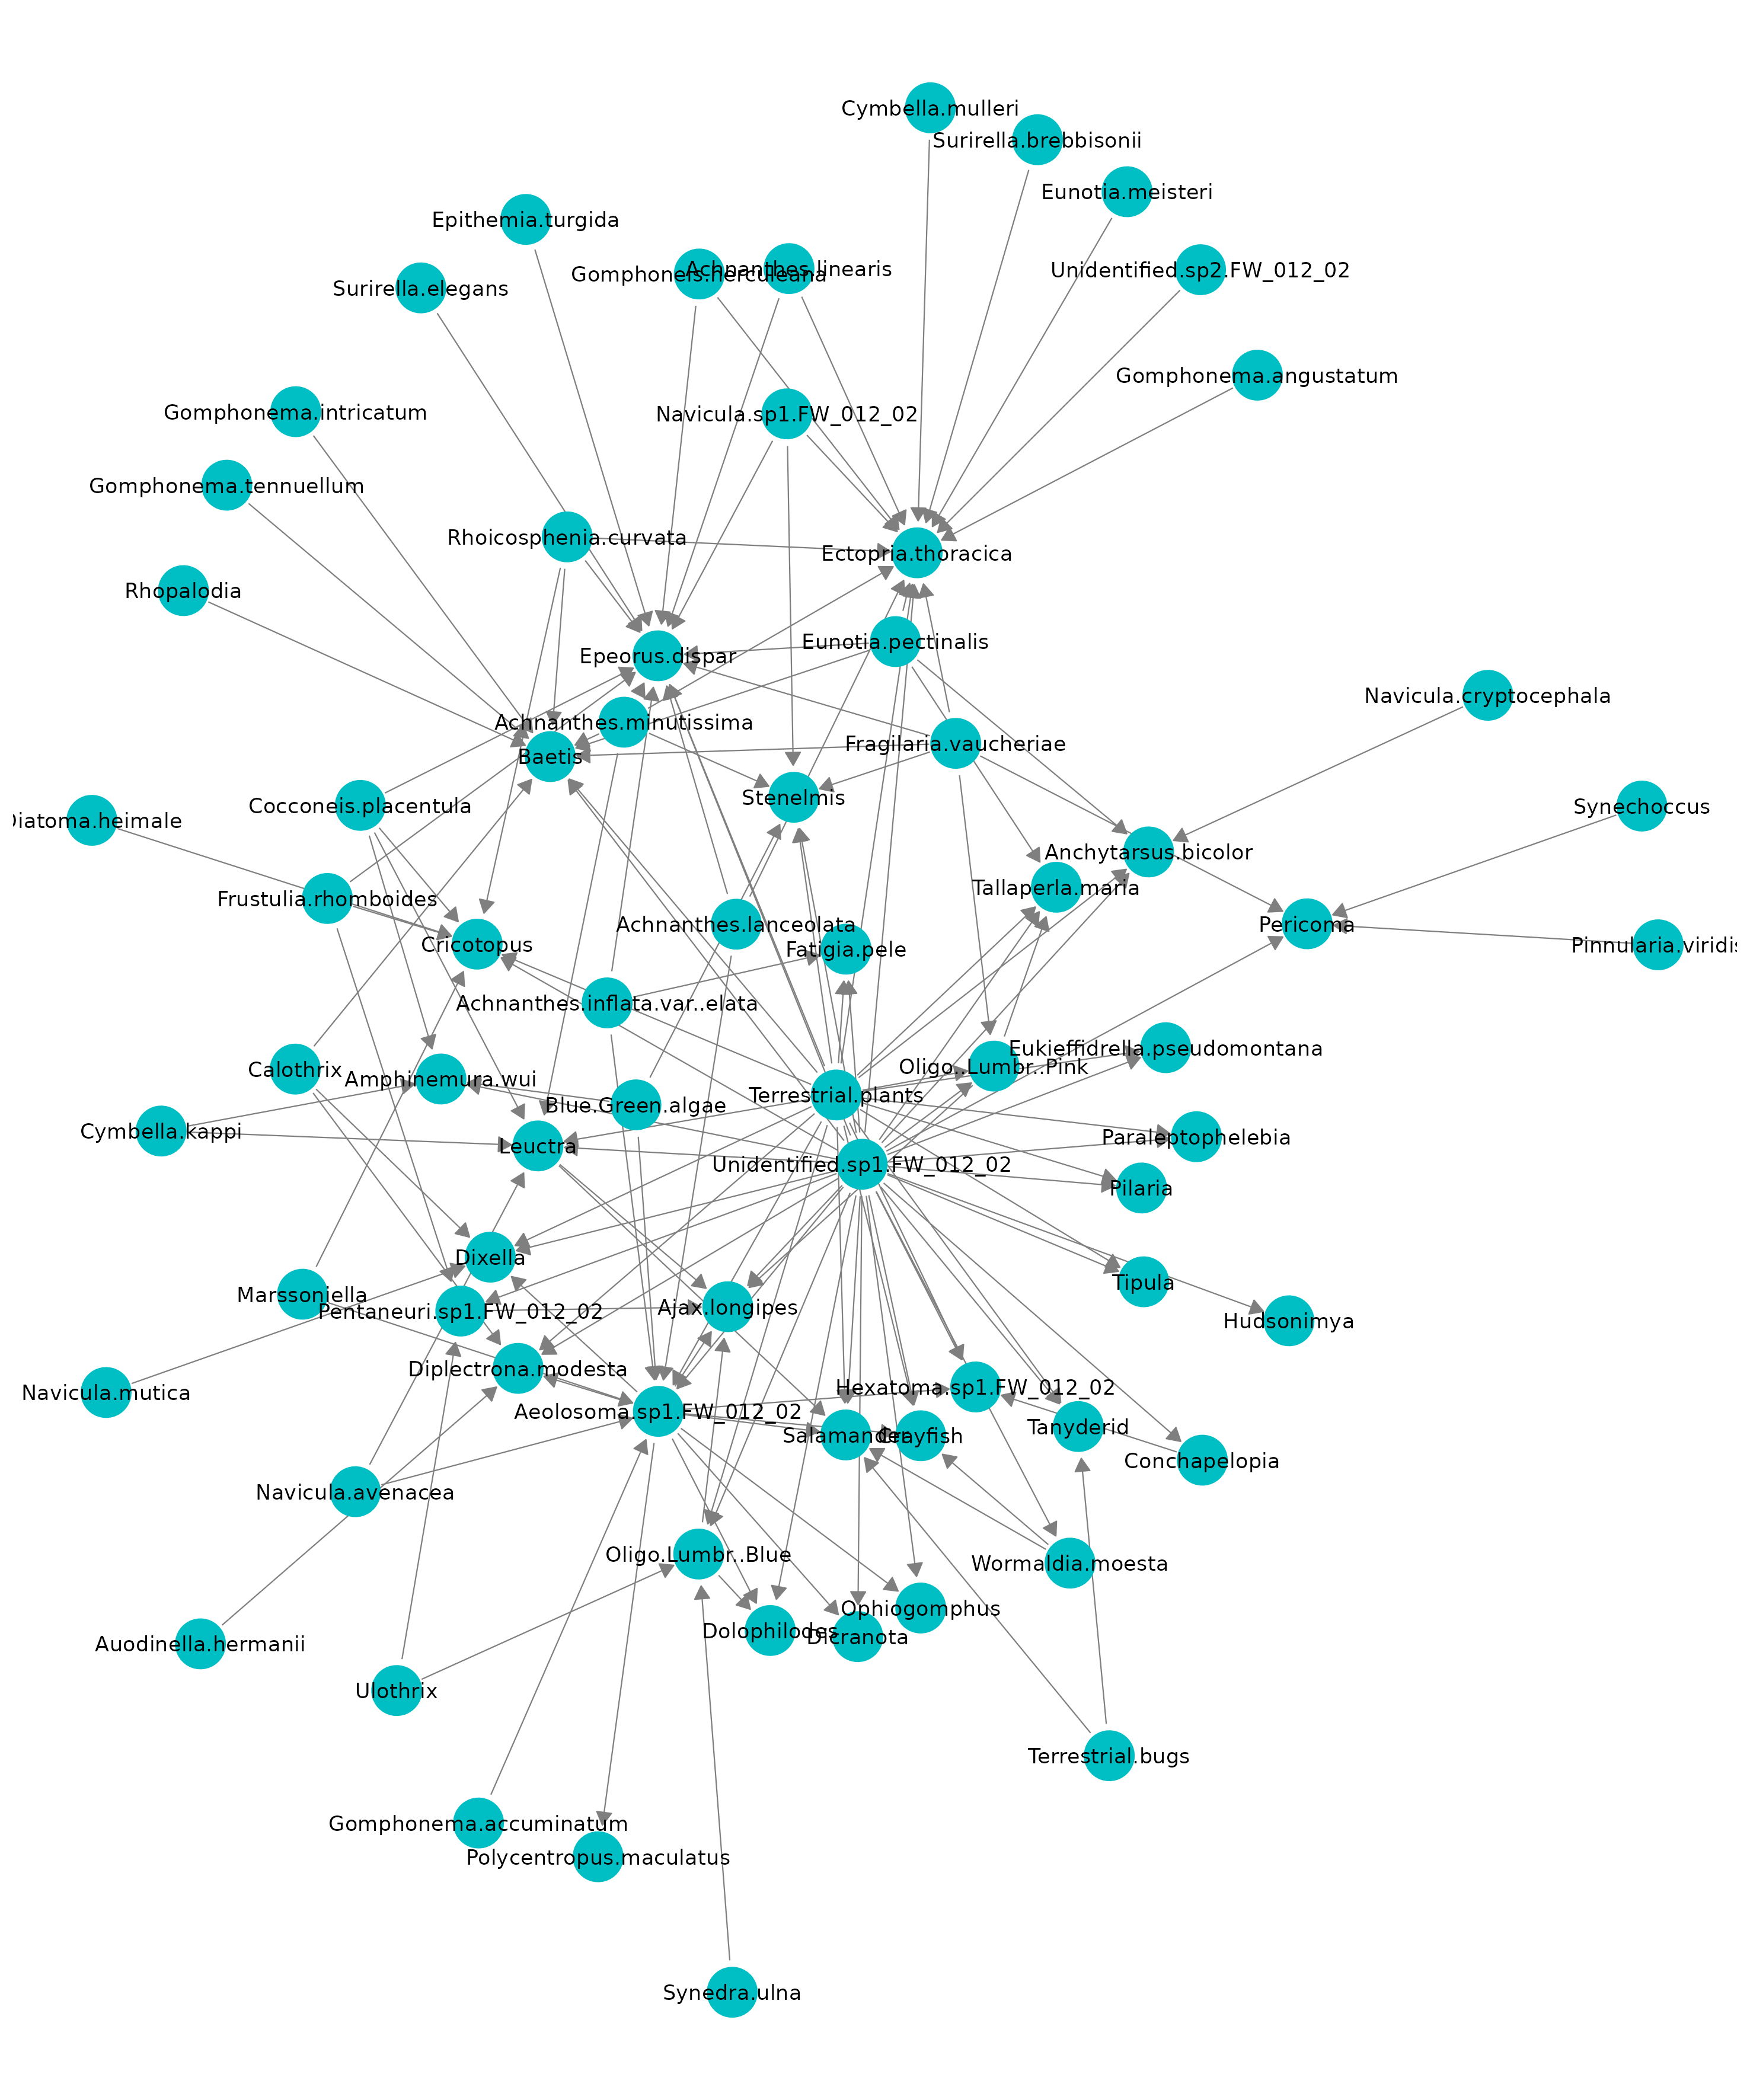
\includegraphics[width=0.7\textwidth]{plots/network_Herlzier(NC)}
\end{column}
\begin{column}{0.5\textwidth}
\centering
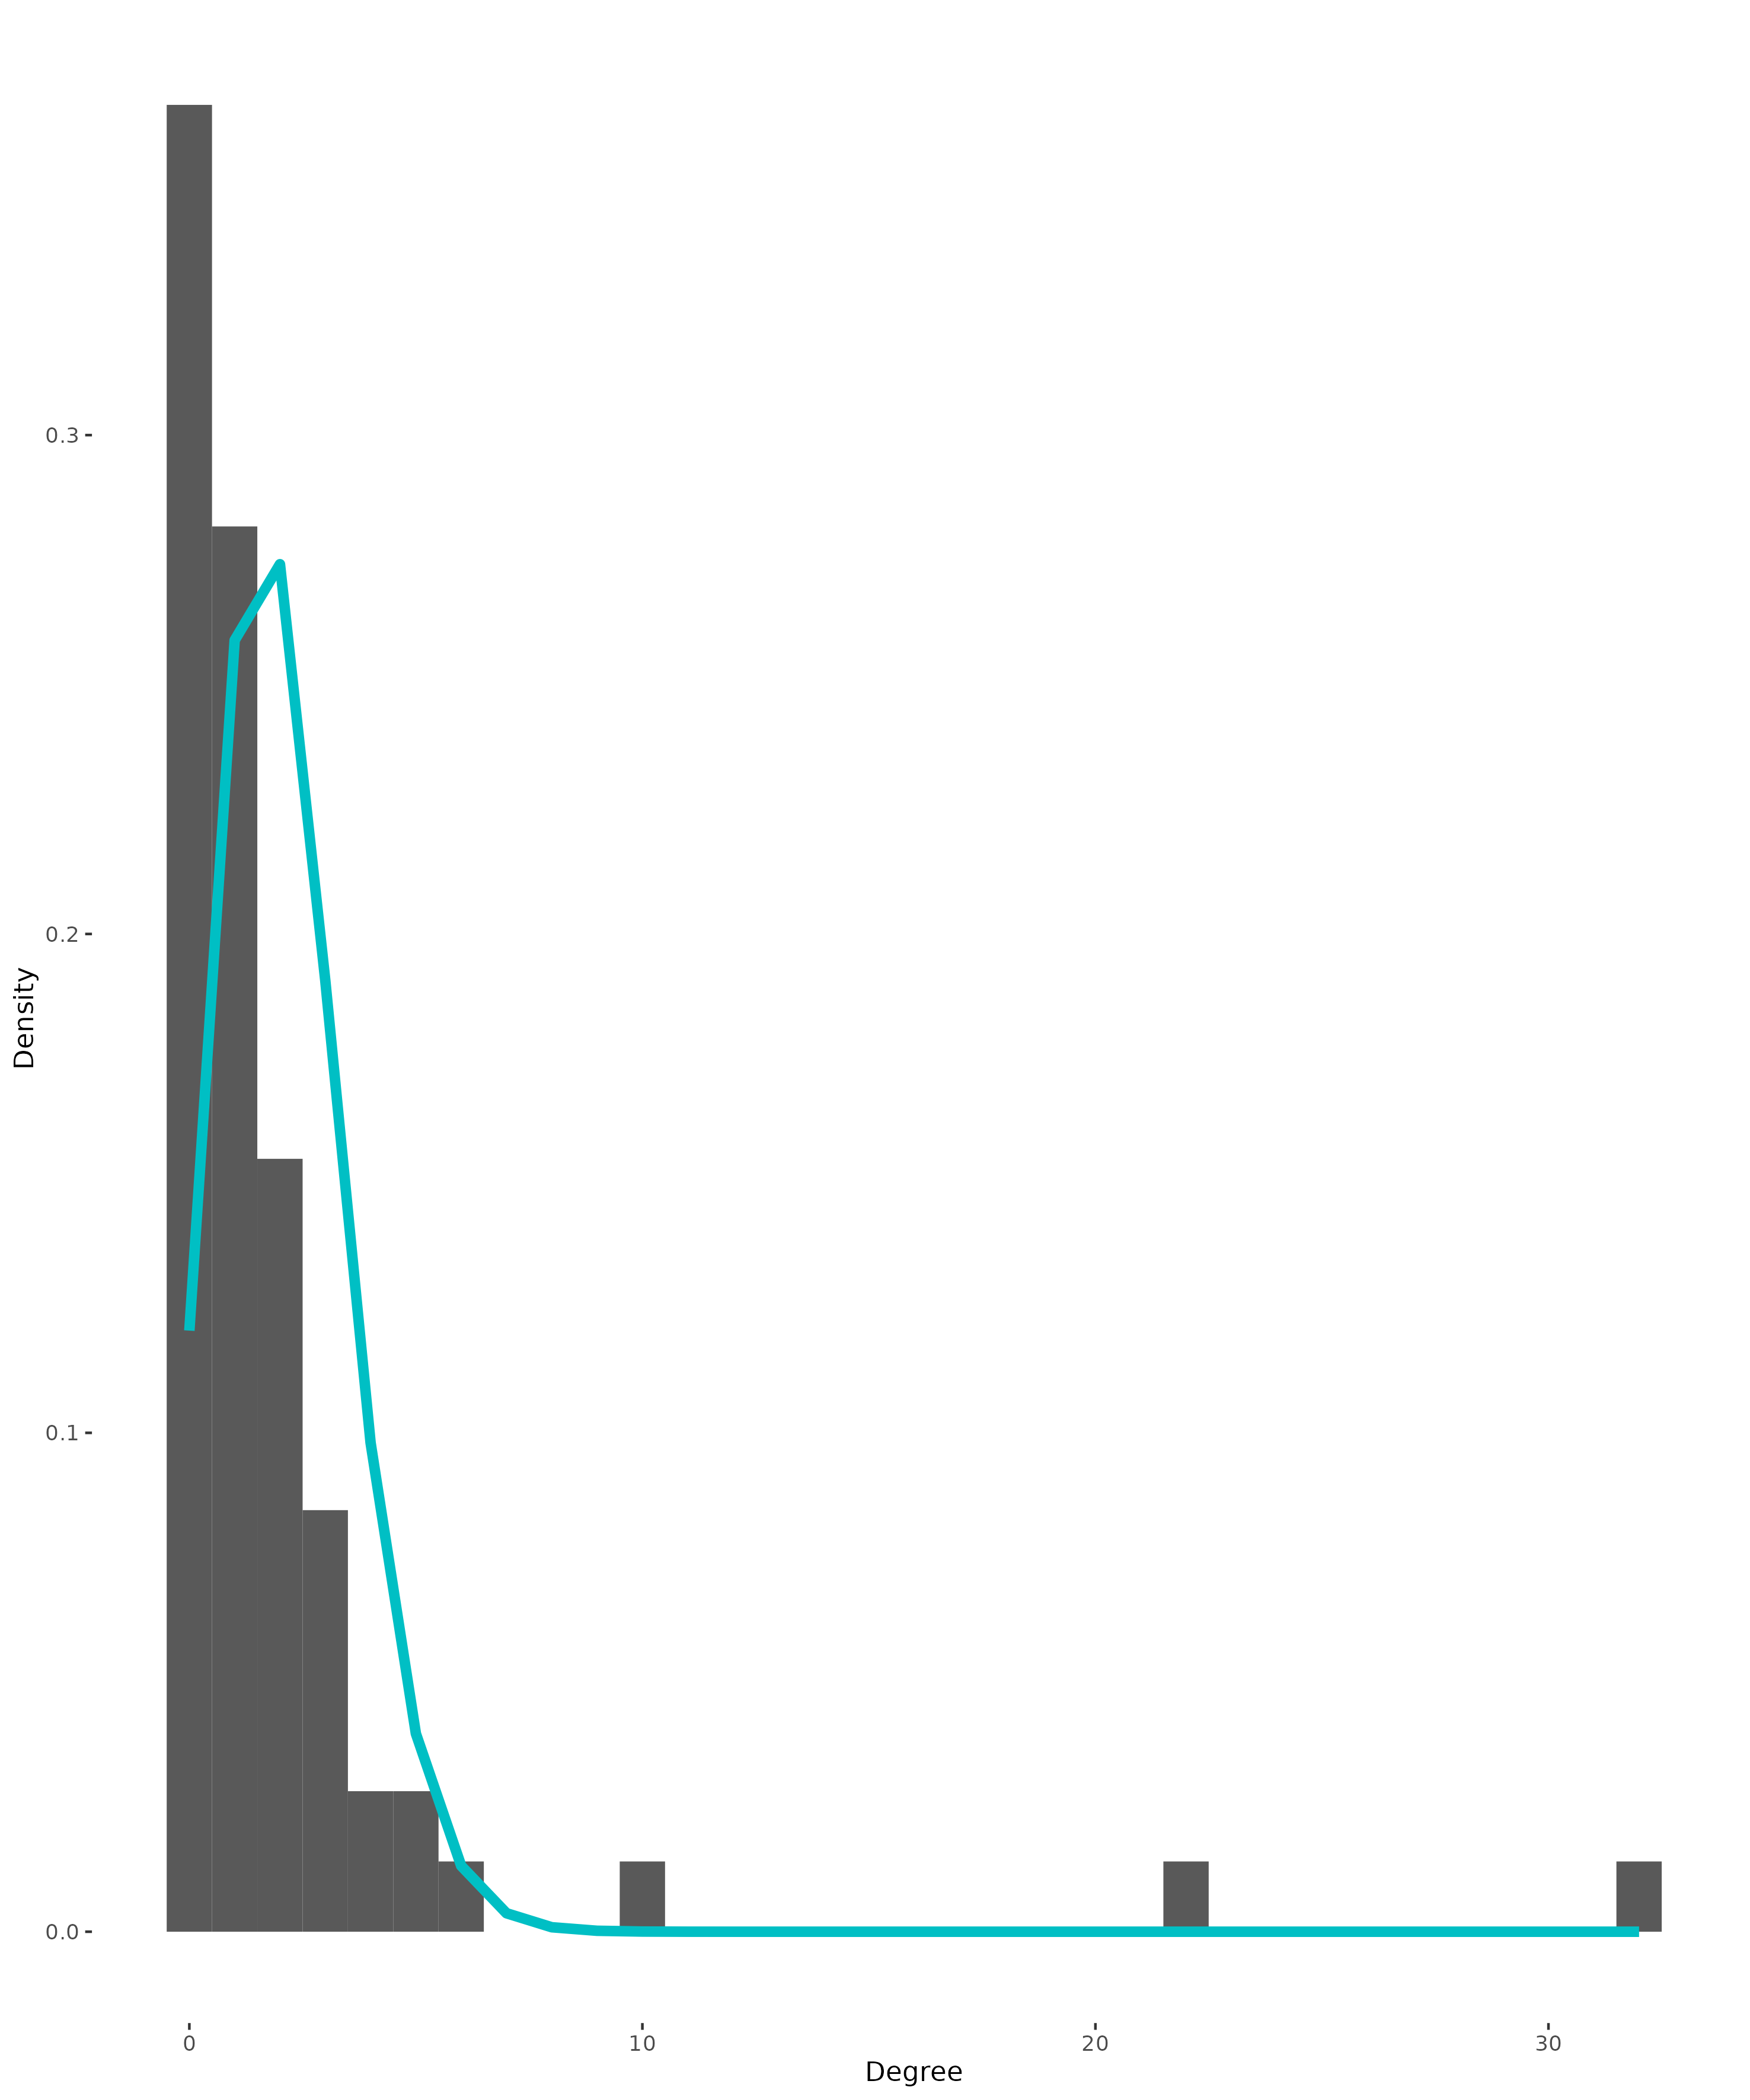
\includegraphics[width=0.7\textwidth]{plots/degree_Herlzier(NC)}
\end{column}
\end{columns}


\bigskip
\centering

 
\centering
Not enough variability in the degree
\end{frame}

%====================================================================
\begin{frame} \frametitle{Limitations of an ER graph to describe real networks}
 %====================================================================

\begin{itemize}
\item  Homogeneity of the connections
 \item Degree distribution too concentrated, no high degree nodes,
 \item All nodes are equivalent (no nestedness...),
 \item No modularity, no hubs
 \end{itemize}

\end{frame}


%====================================================================
\subsection[SBM]{Stochastic Block Model}
%====================================================================

%====================================================================
\begin{frame}  \frametitle{Stochastic Block Model}
%====================================================================
\textcolor{mygreen}{\cite{nowickiSnijders2001}}
Let ($Y_{ij}$) be an adjacency matrix 

\begin{block}{Latent variables}
\begin{itemize}
\item The nodes $i= 1,\dots,n$ are partitionned into $K$ clusters
\item $Z_i = k$ if node $i$ belongs to cluster (block) $k$
\item $Z_i$ independant variables
$$ \mathbb{P}(Z_i = k) = \pi_k$$
\end{itemize}
\end{block}

\begin{block}{Conditionally to $(Z_i)_{i=1,\dots,n}$... }

$(Y_{ij})$ independant and 
\begin{eqnarray*}
 Y_{ij}  | Z_i, Z_j \sim  \mathcal{B}ern(\alpha_{Z_i,Z_j}) \quad \Leftrightarrow \quad  P(Y_{ij} = 1 | Z_i = k, Z_j = \ell)  =  \alpha_{k\ell}
\end{eqnarray*}
\end{block}
 


\end{frame}


%====================================================================
\begin{frame}\frametitle{Stochastic Block Model : illustration}
%====================================================================
  \begin{center}
    \begin{overlayarea}{\textwidth}{.5\textheight}
      \begin{columns}
        \begin{column}{.45\paperwidth}
        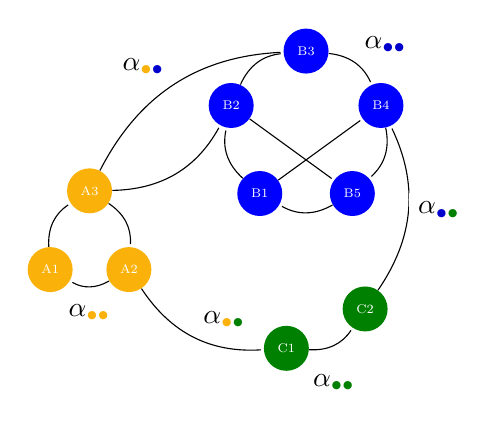
\begin{tikzpicture}
          %% UN GRAPH

          \tikzstyle{every edge}=[-,>=stealth',shorten >=1pt,auto,thin,draw]
          \tikzstyle{every state}=[draw=none,text=white,scale=0.65, font=\scriptsize, transform shape]
          \tikzstyle{every node}=[fill=yellow!40!orange]
          % premier cluster
          \node[state] (A1) at (0,0.5) {A1};
          \node[state] (A2) at (1,0.5) {A2};
          \node[state] (A3) at (.5,1.5) {A3};

          \path (A2) edge [bend left] node[fill=white,below=.1cm]
          {$\alpha_{\textcolor{yellow!40!orange}{\bullet}\textcolor{yellow!40!orange}{\bullet}}$}
          (A1)
          (A1) edge [bend left] (A3)
          (A3) edge [bend left] (A2);

          \tikzstyle{every node}=[fill=blue!80!black]
          \foreach \angle/\text in {234/B1, 162/B2, 90/B3, 18/B4, -54/B5} {
            \node[fill=blue,state,xshift=5cm,yshift=3.5cm]     (\text)    at
            (\angle:1cm) {\text};
          }
          \path (B2) edge (B5)
          (B1) edge (B4);
          \foreach \from/\to in {1/2,2/3,4/5,5/1}{
            \path (B\from) edge [bend left] (B\to);
          }

          \path    (B3)    edge     [bend    left]    node[fill=white]
          {$\alpha_{\textcolor{blue!80!black}{\bullet}\textcolor{blue!80!black}{\bullet}}$}  (B4) ;
          
          \tikzstyle{every node}=[fill=green!50!black]
          % troisieme cluster
          \node[state] (C1) at (3,-.5) {C1};
          \node[state] (C2) at (4,0) {C2};

          \path (C1) edge [bend right] node[fill=white,below=.25cm]
          {$\alpha_{\textcolor{green!50!black}{\bullet}\textcolor{green!50!black}{\bullet}}$}
          (C2);

          % inter cluster
          \path (A3) edge [bend right]  (B2)
          (A3)    edge    [bend    left]    node[fill=white]
          {$\alpha_{\textcolor{yellow!40!orange}{\bullet}\textcolor{blue!80!black}{\bullet}}$}
          (B3)
          (C2) edge [bend right] node[fill=white,right]
          {$\alpha_{\textcolor{blue!80!black}{\bullet}\textcolor{green!50!black}{\bullet}}$}
          (B4)
          (A2) edge [bend right] node[fill=white]
          {$\alpha_{\textcolor{yellow!40!orange}{\bullet}\textcolor{green!50!black}{\bullet}}$}
          (C1);
        \end{tikzpicture}
        \end{column}


        \begin{column}{.5\paperwidth}
          \begin{small}
            \begin{block}{Parameters}
              Let $n$ nodes divided into $3$ clusters
              \begin{itemize}
              \item
                $\mathcal{K}=\{\textcolor{yellow!40!orange}{\bullet},\textcolor{blue!80!black}{\bullet},\textcolor{green!50!black}{\bullet}\}$
                 clusters
              \item  $\pi_\bullet  =  \mathbb{P}(i  \in  \bullet)$,
                $\bullet\in\mathcal{K},i=1,\dots,n$
              \item      $\alpha_{\textcolor{yellow!40!orange}{\bullet}\textcolor{blue!80!black}{\bullet}}     =      \mathbb{P}(i
                \leftrightarrow j | i\in\textcolor{yellow!40!orange}{\bullet},j\in\textcolor{blue!80!black}{\bullet})$
              \end{itemize}
            \end{block}
          \end{small}
        \end{column}
      \end{columns}
    \end{overlayarea}
  \end{center}
  
\begin{align*}
Z_i = \mathbf{1}_{\{i \in \bullet\}}  \ & \sim^{\text{iid}} \mathcal{M}(1,\pi), \quad \forall\bullet \in \mathcal{K}, \\ 
Y_{ij} \ | \ \{i\in\textcolor{yellow!40!orange}{\bullet},j\in\textcolor{blue!80!black}{\bullet}\}
& \sim^{\text{ind}} \mathcal{B}(\alpha_{\textcolor{yellow!40!orange}{\bullet}\textcolor{blue!80!black}{\bullet}})\\
\end{align*}

\end{frame}


%====================================================================
\begin{frame}\frametitle{SBM : A great generative model}
%====================================================================
\begin{itemize}
\item  Generative model : easy to simulate
\item No a priori on the type of structure
\item Combination of modularity, nestedness, etc... 
\end{itemize}


\alert{References}
\begin{itemize}
 \item Other ways to model heterogeneity in networks \textcolor{mygreen}{\cite{matias2014ESAIM}}
\item Review paper on SBM \textcolor{mygreen}{\cite{Lee2019}}
\end{itemize}


\end{frame}

%====================================================================
\frame{\frametitle{Modelling communities} 
%====================================================================
$$p  = \left( 
\begin{array}{ccc}
\underline{0.45}& 0.05& 0.05\\
0.05&\underline{0.45} & 0.05\\
0.05& 0.05& \underline{0.45}
\end{array}
\right) \quad \quad \nu = (0.25,0.5,0.25)
$$ 

\begin{columns}
\begin{column}{0.5\textwidth}
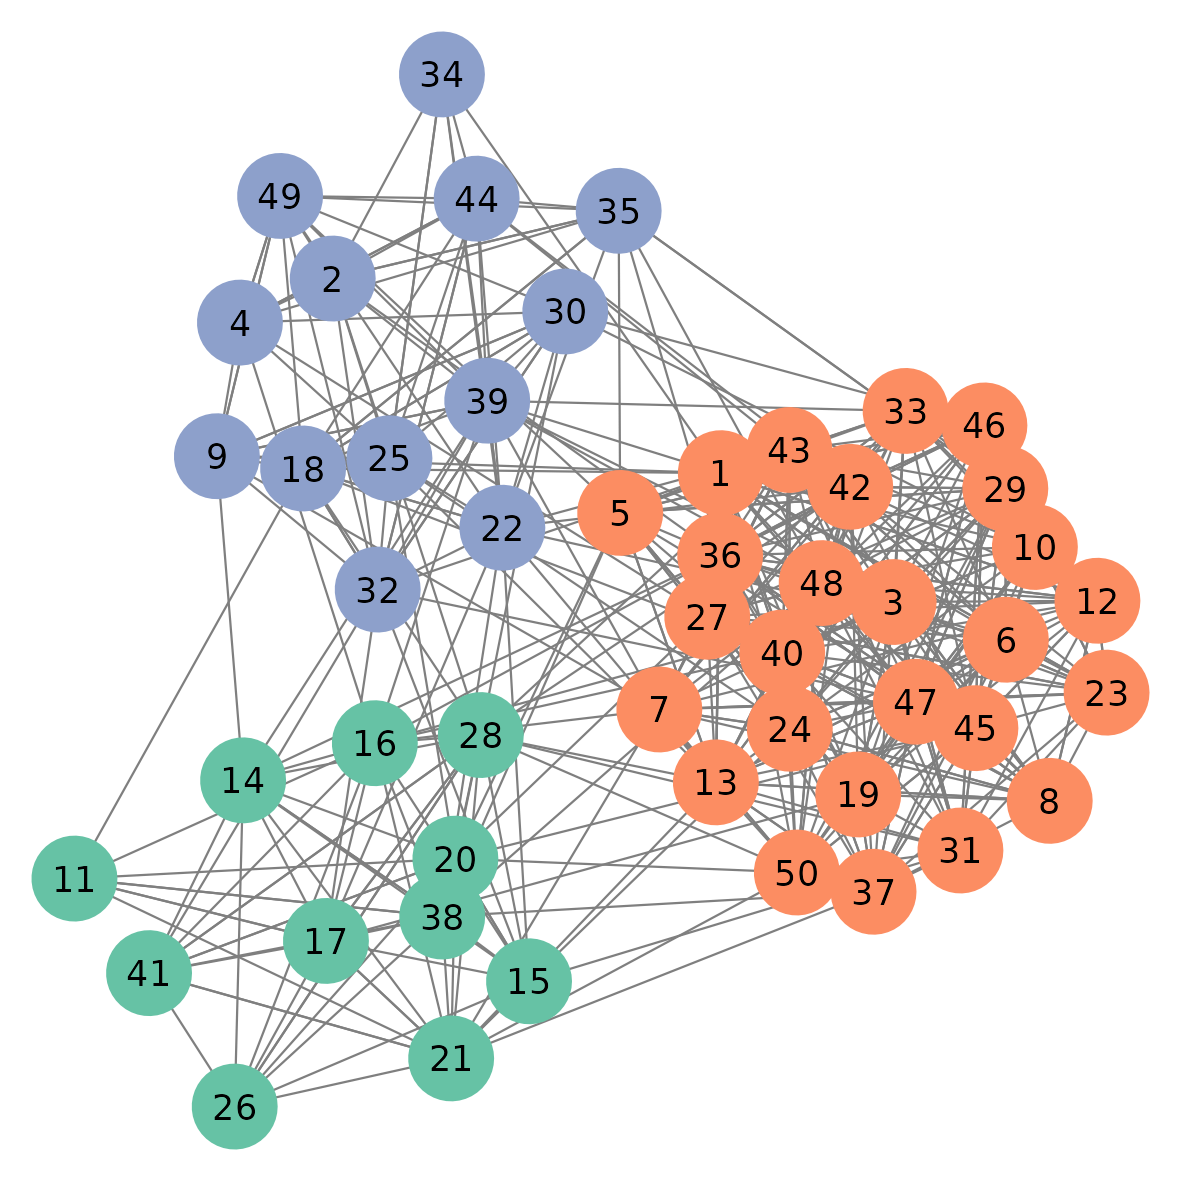
\includegraphics[width=\textwidth]{plots/network_SimuCommunities}
\end{column}
\begin{column}{0.5\textwidth}
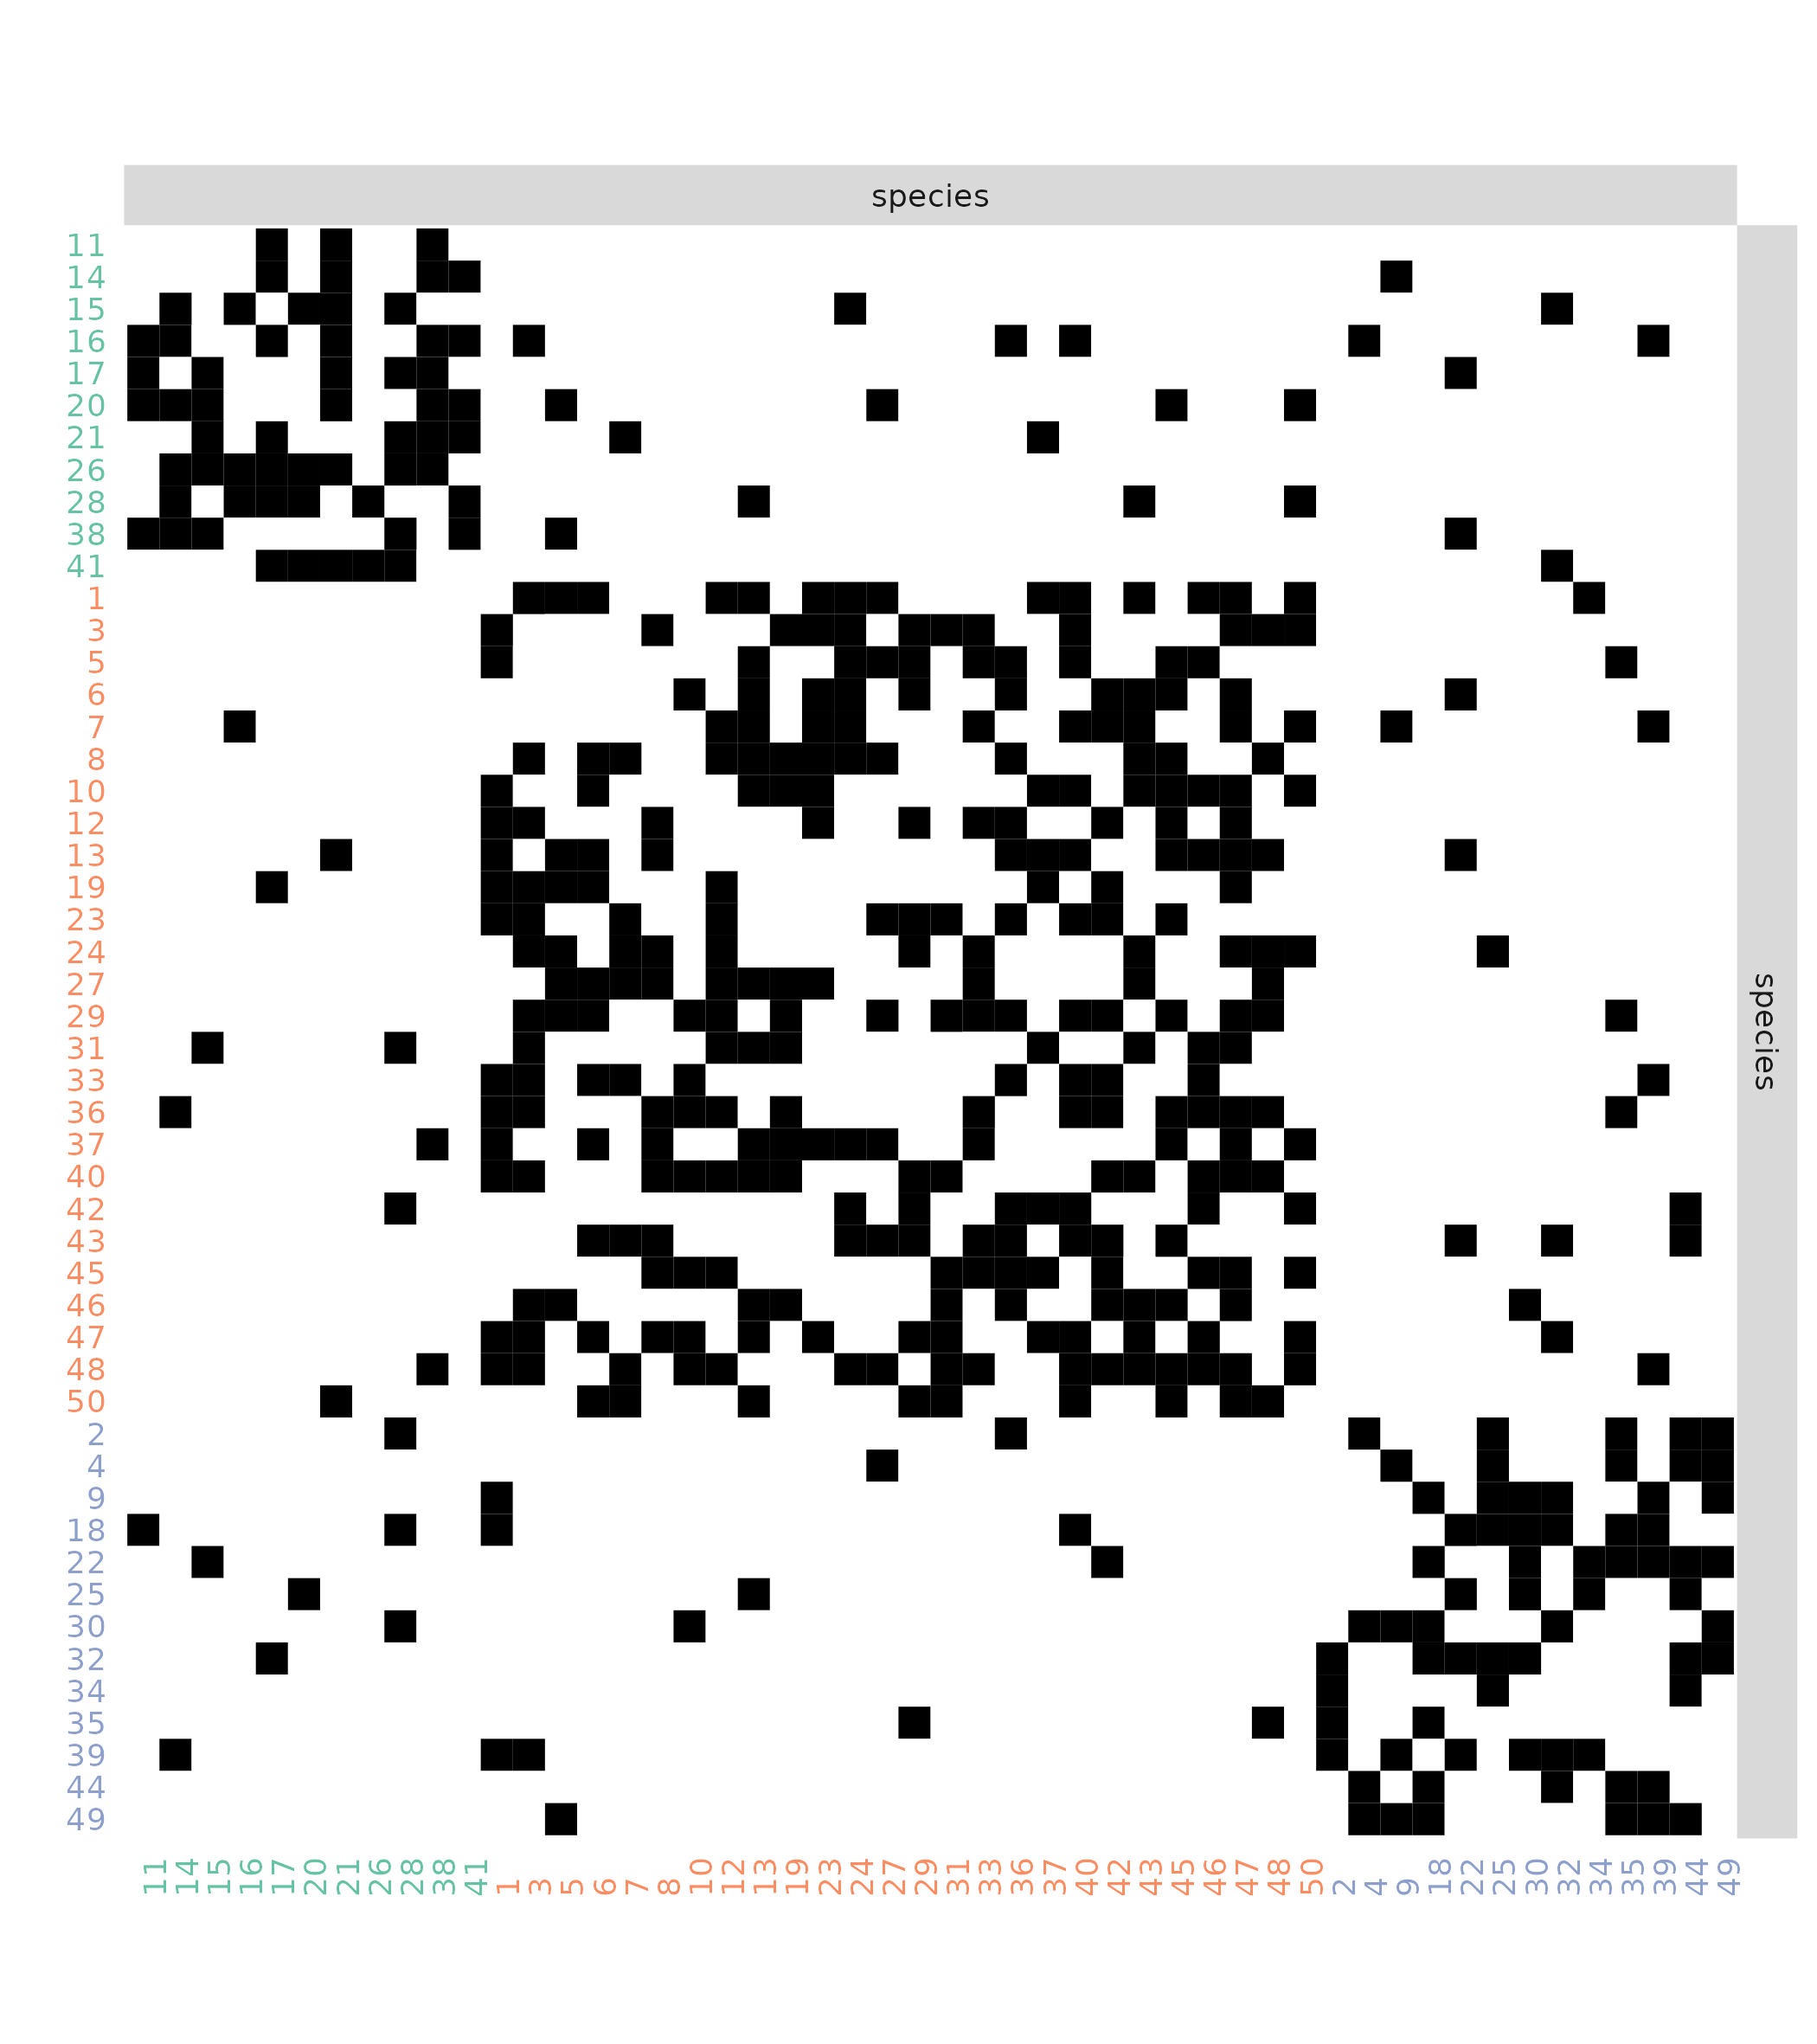
\includegraphics[width=0.9\textwidth]{plots/matrix_SimuCommunities}
\end{column}
\end{columns}
}


%====================================================================
\frame{\frametitle{Modelling foodwebs} 
%====================================================================
$$p  = \left( 
\begin{array}{cccc}
0.10  & 0.02 &0.02 &0.02\\
\underline{0.50} &0.10& 0.02& 0.02\\
\underline{0.50} &\underline{0.40} &0.10& 0.02\\
0.02 &\underline{0.40}& \underline{0.40} & 0.10 
\end{array}
\right) \quad \quad \nu = (0.2, .25, 0.30 ,0.25)
$$ 
\vspace{-2em}
\begin{columns}
\begin{column}{0.5\textwidth}
\includegraphics[width=\textwidth]{plots/network_SimuFoodweb}
\end{column}
\begin{column}{0.5\textwidth}
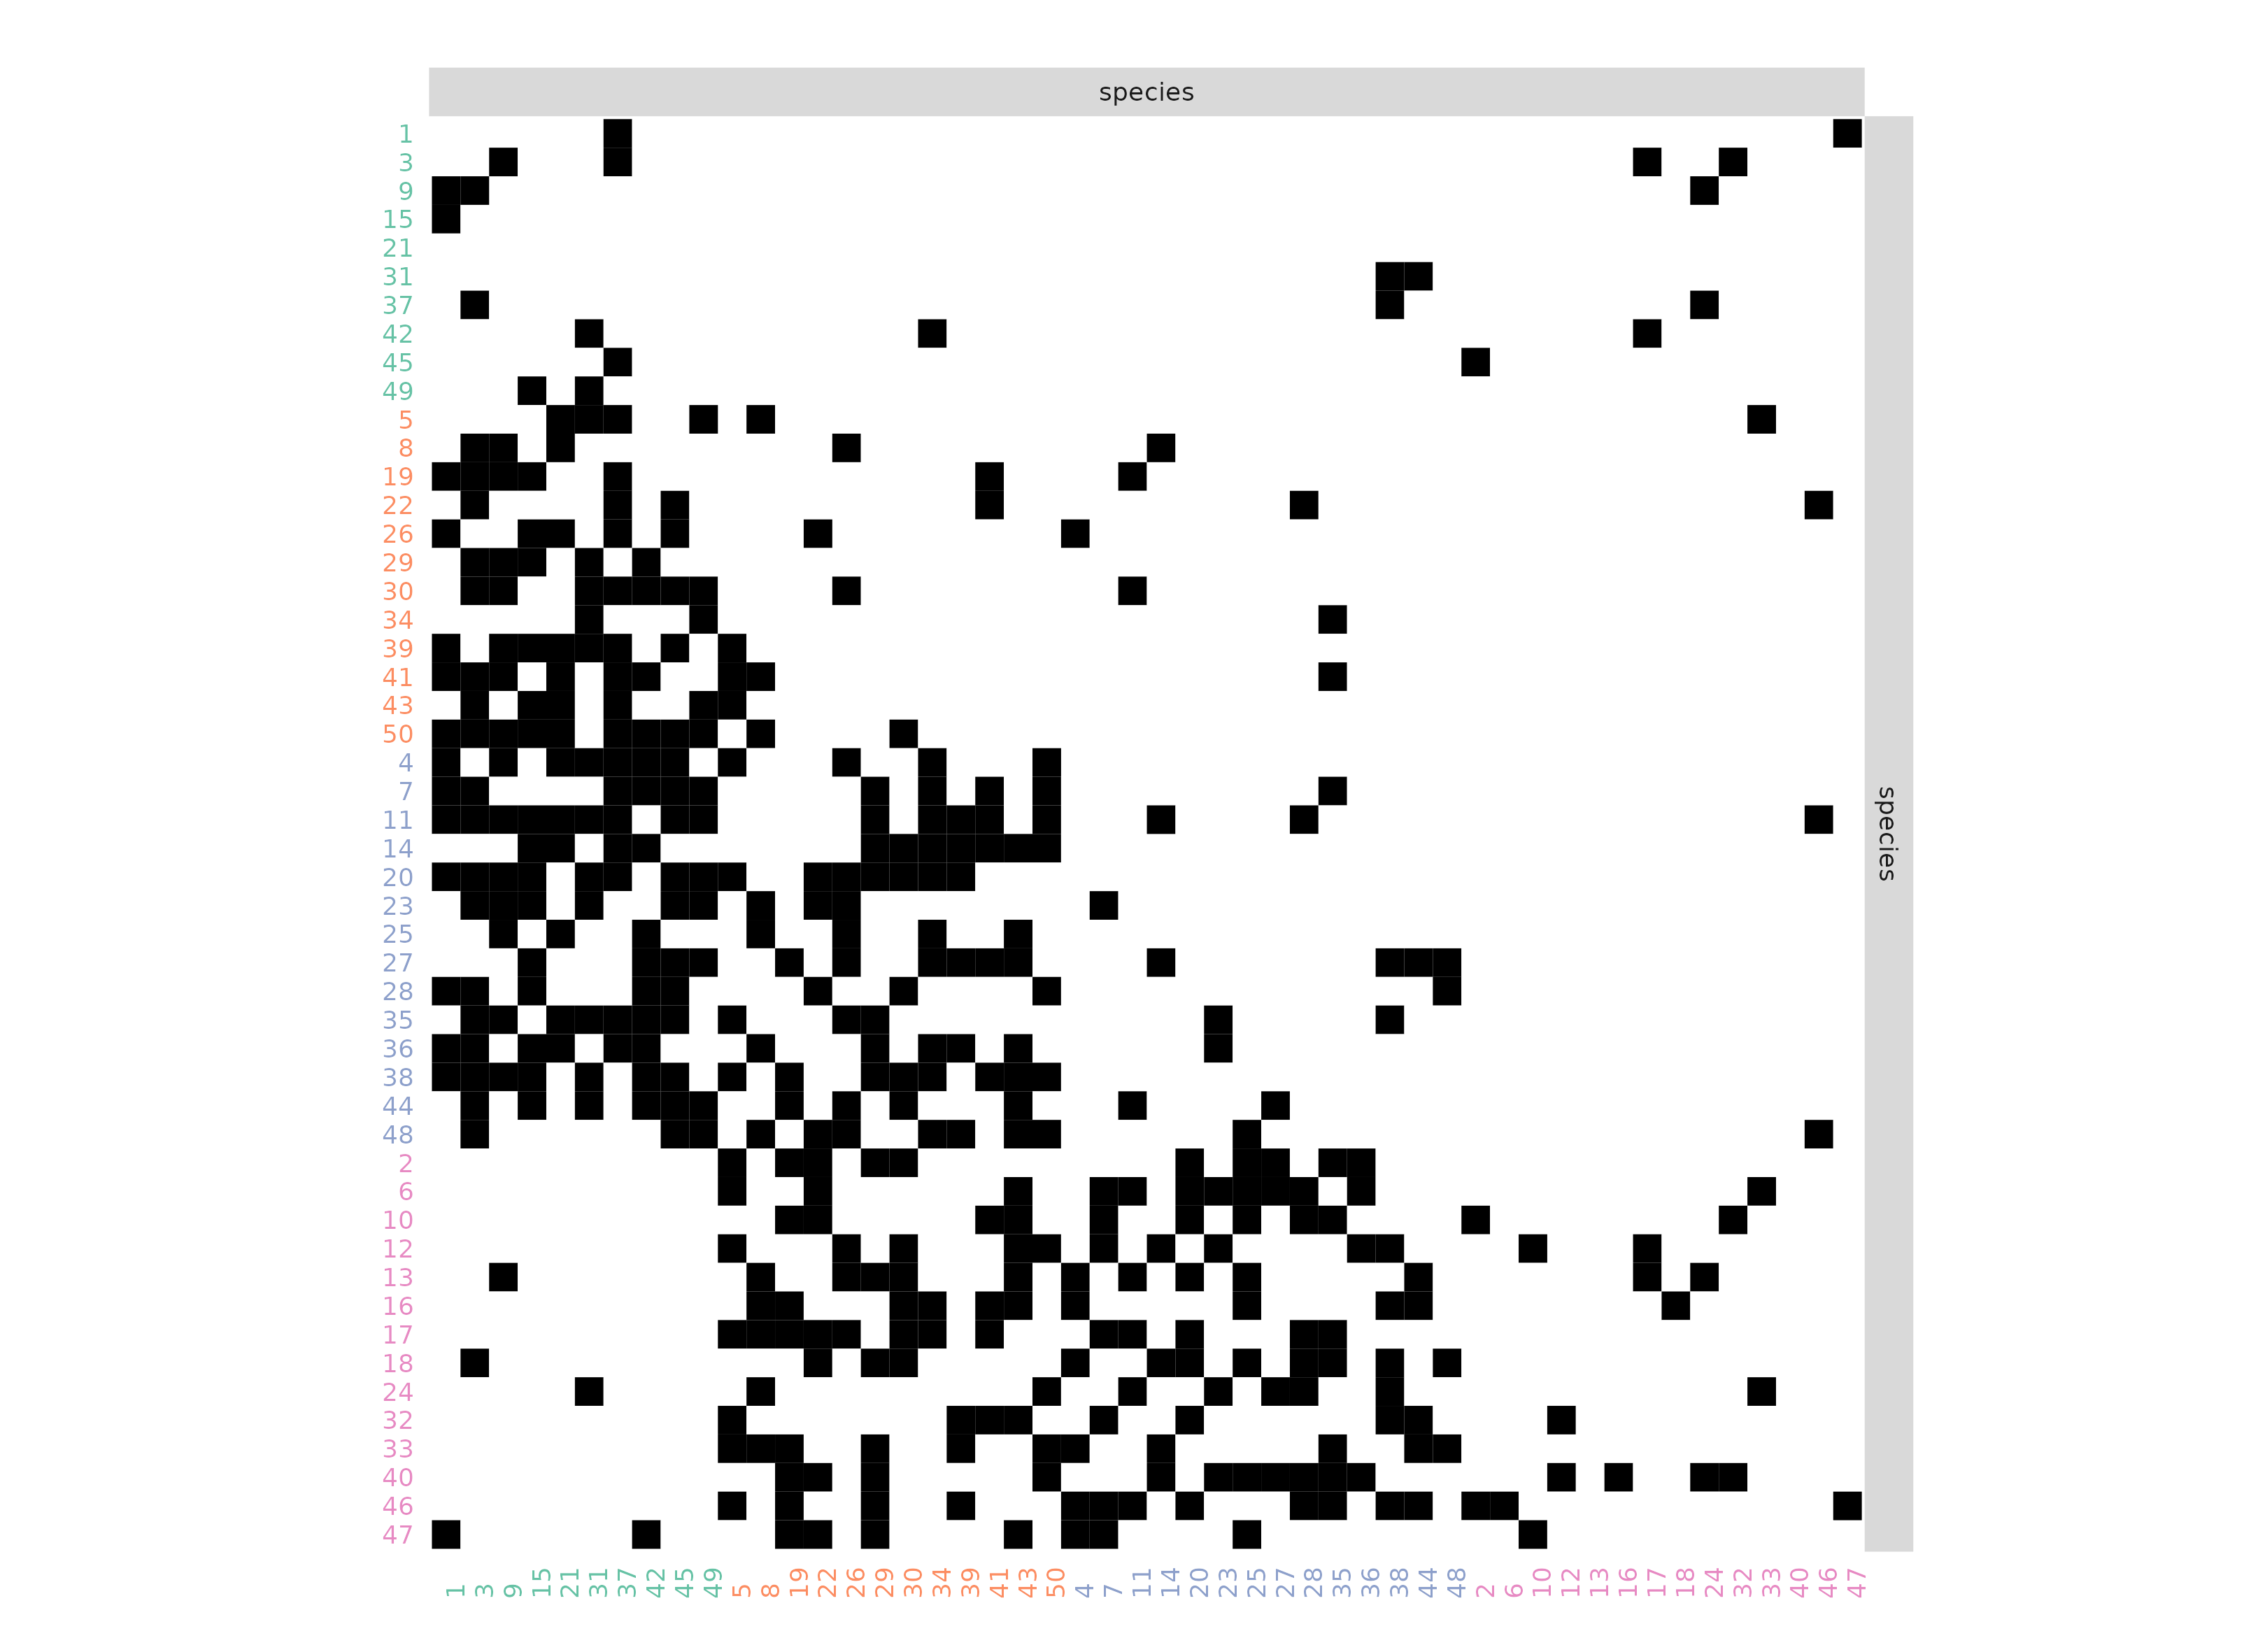
\includegraphics[width=0.9\textwidth]{plots/matrix_SimuFoodWeb}
\end{column}
\end{columns}
}



%====================================================================
\subsection[LBM]{Bipartite stochastic block models}
%====================================================================

%====================================================================
\begin{frame}{Probabilistic model for binary  bipartite networks}
%====================================================================

\includegraphics[width=0.8\textwidth]{plots/Tree_fungis_matrix}


\centering
Requires adaptation to bipartite networks: blocks for rows and cols
\end{frame}


%====================================================================
\begin{frame}{Probabilistic model for binary  bipartite networks}
%====================================================================

Let $Y_{ij}$ be a bi-partite network. Individuals in row and cols are not the same. 

\begin{block}{Latent variables : bi-clustering}
\begin{itemize}
\item Nodes $i= 1,\dots,n$   partitionned into $K$ clusters,  nodes $j= 1,\dots,p$  partitionned into $L$ clusters
\item $$\begin{array}{cl}
Z_i = k & \mbox{if node $i$ belongs to cluster (block) $k$}\\
W_j = \ell & \mbox{if node $j$ belongs to cluster (block) $\ell$}
\end{array}$$
\item $(Z_i)_{i=1,\dots,n}, (W_j)_{j=1, \dots,p}$ independent variables
$$ \mathbb{P}(Z_i = k) = \pi_k,\quad  \mathbb{P}(W_j = \ell) = \rho_\ell$$
\end{itemize}
\end{block}

\end{frame}

%====================================================================
\begin{frame}{Probabilistic model for binary  bipartite networks}
%====================================================================

\begin{block}{Conditionally to $(W_i)_{i=1,\dots,n},(W_j)_{j=1,\dots,p}$... }

$(Y_{ij})$ independent and 
\begin{eqnarray*}
 Y_{ij}  | Z_i, W_j \sim  \mathcal{B}ern(\alpha_{Z_i,W_j}) \quad \Leftrightarrow \quad   \mathbb{P}(Y_{ij} = 1 | Z_i = k, W_j = \ell)  =  \alpha_{k\ell}
\end{eqnarray*}
\end{block}
 

 Also called Latent Block Models
\textcolor{mygreen}{\cite{Govaert2008}}

\end{frame}

%-------------------------------------------------------------------------------------
% 
% 
% \begin{frame}
% \frametitle{Latent Block Model : illustration}
% 
%  \begin{center}
%     \begin{overlayarea}{\textwidth}{.5\textheight}
%       \begin{columns}
%         \begin{column}{.45\paperwidth}
%         \centering
%         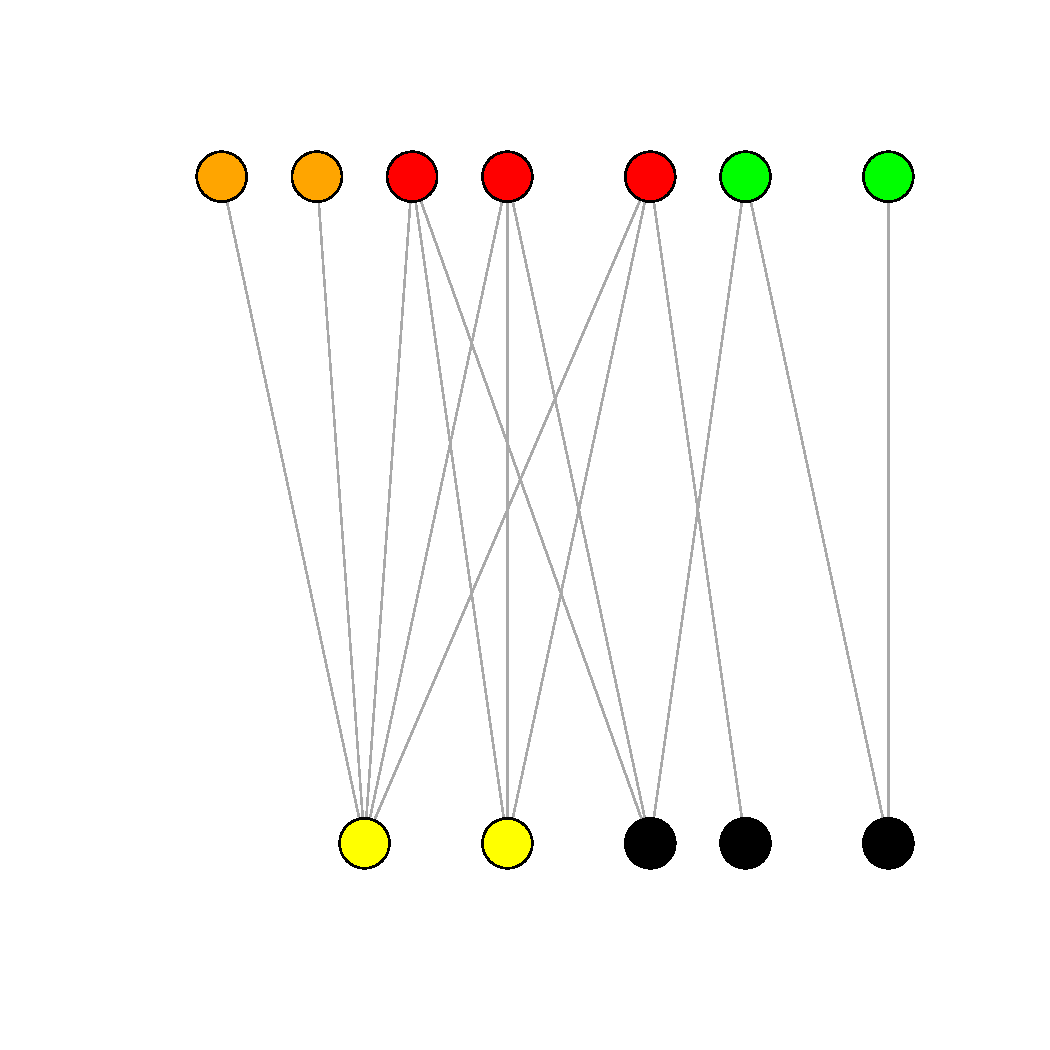
\includegraphics[scale=.3]{plots/LBM_exemple.pdf}
%         \end{column}
%         \begin{column}{.5\paperwidth}
%           \begin{small}
%             \begin{block}{Latent Block Model}
%               \begin{itemize}
%               \item
%                 $n_1$ row nodes $\mathcal{K}_1=\{\textcolor{red}{\bullet},\textcolor{orange}{\bullet},\textcolor{green}{\bullet}\}$
%                 classes
%               \item  $\pi^1_\bullet  =  \mathbb{P}(i  \in  \bullet)$,
%                 $\bullet\in\mathcal{K}_1,i=1,\dots,n$
%               \item $n_2$ column nodes $\mathcal{K}_2=\{\textcolor{yellow}{\bullet},\textcolor{black}{\bullet}\}$
%                 classes
%                \item  $\pi^2_\bullet  =  \mathbb{P}(j  \in  \bullet)$,
%                 $\bullet\in\mathcal{K}_2,j=1,\dots,m$
%               \item      $\alpha_{\textcolor{red}{\bullet}\textcolor{yellow}{\bullet}}     =      \mathbb{P}(i
%                 \leftrightarrow j | i\in\textcolor{red}{\bullet},j\in\textcolor{yellow}{\bullet})$
%               \end{itemize}
%             \end{block}
%           \end{small}
%         \end{column}
%       \end{columns}
%     \end{overlayarea}
%   \end{center}
%   
% %\begin{eqnarray*}
% %&(Z_i) &  \ \sim^{\text{iid}} \mathcal{M}(1,\alpha) \ \text{et} \  Z_{i} \in \{1,...,Q\}, \\ 
% % &(Y_{ij})&| \ \{Z_{i},Z_{j}\} \sim^{\text{ind}} \mathcal{B}(\pi_{Z_{i}Z_{j}}).\\
% %\end{eqnarray*}
% 
% % Proposition Julien
% \begin{align*}
% Z_i = \mathbf{1}_{\{i \in \bullet\}}  \ & \sim^{\text{iid}} \mathcal{M}(1,\bpi^1), \quad \forall\bullet \in \mathcal{Q}_1, \\ 
% W_j=\mathbf{1}_{\{j \in \bullet\}}  \ & \sim^{\text{iid}} \mathcal{M}(1,\bpi^2), \quad \forall\bullet \in \mathcal{Q}_2, \\
% Y_{ij} \ | \ \{i\in\textcolor{red}{\bullet},j\in\textcolor{yellow}{\bullet}\}
% & \sim^{\text{ind}} \mathcal{B}ern(\alpha_{\textcolor{red}{\bullet}\textcolor{yellow}{\bullet}})\\
% \end{align*}
% 
% 
% \textcolor{mygreen}{\cite{Govaert2008}} and 
% \textcolor{mygreen}{R package: blockmodels} as well.
% 
% \end{frame}





%====================================================================
\subsection{Some possible extensions}
%====================================================================
\begin{frame} \frametitle{Valued-edge networks}
%====================================================================

\begin{block}{Values-edges networks}
 Information on edges can be something different from presence/absence.
 It can be:
 \begin{enumerate}
  \item a count of the number of observed interactions,
  \item a quantity interpreted as the interaction strength,
  \end{enumerate}

 \end{block}

 \bigskip
 
 


\begin{block}{ Natural extensions of SBM and LBM}
 \begin{enumerate}
  \item Poisson distribution: $Y_{ij} \ | \ \{i\in\textcolor{yellow!40!orange}{\bullet},j\in\textcolor{blue!80!black}{\bullet}\}
\sim^{\text{ind}} \mathcal{P}(\lambda_{\textcolor{yellow!40!orange}{\bullet}\textcolor{blue!80!black}{\bullet}})$,
 \item Gaussian distribution: $Y_{ij} \ | \ \{i\in\textcolor{yellow!40!orange}{\bullet},j\in\textcolor{blue!80!black}{\bullet}\}
\sim^{\text{ind}} \mathcal{N}(\mu_{\textcolor{yellow!40!orange}{\bullet}\textcolor{blue!80!black}{\bullet}},\sigma^2)$,
\textcolor{mygreen}{\cite{mariadassou2010uncovering}}
\item More generally, 
  $$Y_{ij} \ | \ \{i\in\textcolor{yellow!40!orange}{\bullet},j\in\textcolor{blue!80!black}{\bullet}\}
\sim^{\text{ind}} \mathcal{F}(\theta_{\textcolor{yellow!40!orange}{\bullet}\textcolor{blue!80!black}{\bullet}})$$
 \end{enumerate}
 \end{block}
 \bigskip

\end{frame}

%====================================================================
\begin{frame} \frametitle{Multiplex networks}
%====================================================================
Several kind of interactions between nodes
For instance : 


\begin{itemize}
\item Love and friendship
\item Working relations and friendship
\item  In ecology : mutualistic and competition
\end{itemize}


\begin{block}{Block model for multiplex networks}

$Y_{ij} \in \{0,1\} ^ Q = (Y_{ij}^a, Y_{ij}^b)$, $\forall w \in \{0,1\}^2$ 



$$\mathbb{P}((Y^a_{ij},Y^b_{ij}) = w  | Z_i  = k, Z_j = \ell)  = \alpha^w _{k\ell}$$

\end{block}

\textcolor{mygreen}{
\cite{kefi}, \cite{barbillon2017stochastic}}

In \textcolor{mygreen}{R package: sbm} when two relations are at stake.
 

 \textbf{Remark:} a particular case of multiplex network is dynamic network, \textcolor{mygreen}{\cite{matias2017statistical}}.
 

 \end{frame}
%====================================================================
\begin{frame}\frametitle{Taking into account covariates}
%====================================================================
 Sometimes covariates are available. They may be on:
 \begin{itemize}
  \item nodes,
  \item edges,
  \item both.
 \end{itemize}

 
 
 \begin{enumerate}
  \item They can be used a posteriori to explain blocks inferred by SBM.
  \item Extension of the SBM which takes into account covariates. Blocks are structure of interaction which is not 
  explained by covariates !

 \end{enumerate}


 If covariates are sampling conditions, case 2  be  may more interesting.
 
\end{frame}

%====================================================================
\begin{frame} \frametitle{SBM with covariates}
%====================================================================

\begin{itemize}
\item As before :  ($Y_{ij}$) be an adjacency matrix 
\item  Let   $x^{ij} \in \mathbb{R}^p$  denote covariates describing the pair $(i,j)$
\end{itemize}

\begin{block}{Latent variables : as before }
\begin{itemize}
\item The nodes $i= 1,\dots,n$ are partitioned into $K$ clusters
\item $Z_i$ independent variables
$$ \mathbb{P}(Z_i = k) = \pi_k$$
\end{itemize}
\end{block}
 
\begin{block}{Conditionally to $(Z_i)_{i=1,\dots,n}$... }

$(Y_{ij})$ independent and 
\begin{eqnarray*}
 Y_{ij}  | Z_i, Z_j&\sim&   \mathcal{B}ern(\mbox{logit}(\alpha_{Z_i,Z_j} + \theta \cdot x_{ij}) ) \quad \mbox {if binary data} \\
 Y_{ij}  | Z_i, Z_j  &\sim&  \mathcal{P}(\exp(\alpha_{Z_i,Z_j} + \theta  \cdot x_{ij}) ) \quad \mbox {if counting data} 
\end{eqnarray*}
\end{block}


If $K = 1$ : all the connection heterogeneity is explained by the covariates. 
 \end{frame}

 
 
 
 
 
 
%====================================================================
\section{Inference}
%====================================================================

\begin{frame}{Aim}
 
\alert{Going from... } 

\centering
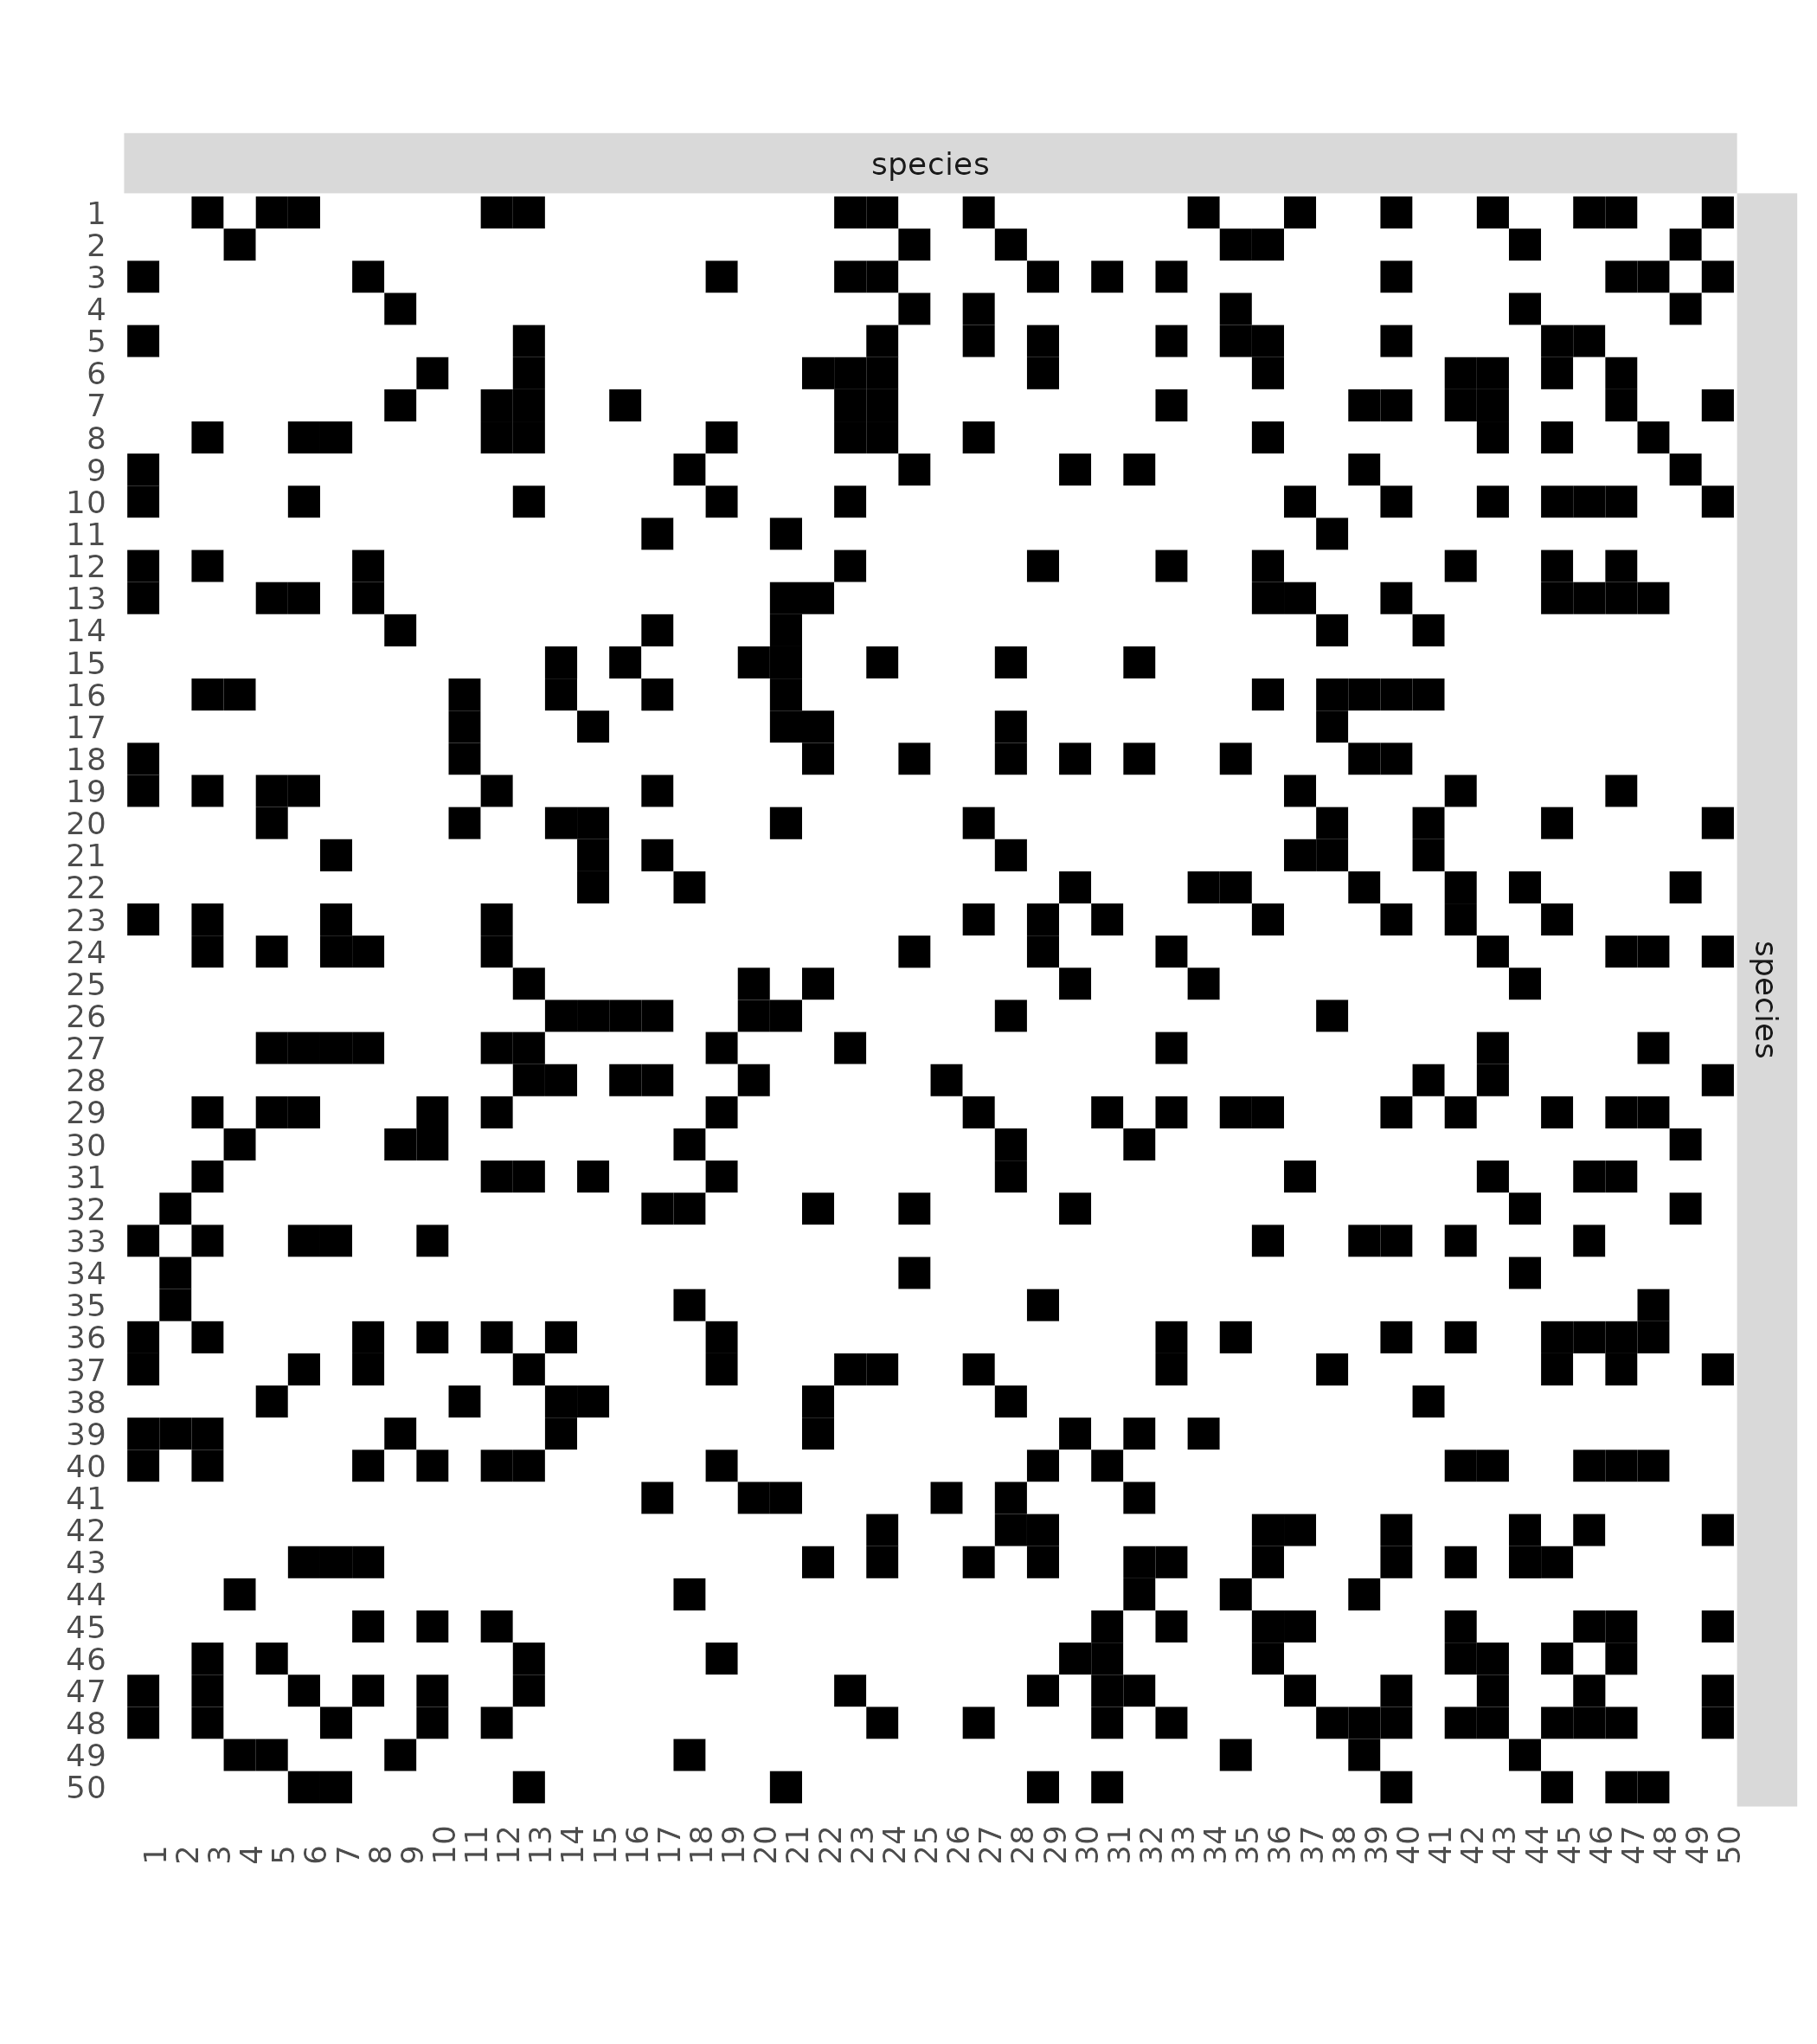
\includegraphics[width=0.5 \textwidth]{plots/matrix_raw}

 
\end{frame}
%====================================================================
\begin{frame}{Aim}
 %====================================================================
\alert{... to} 

\centering

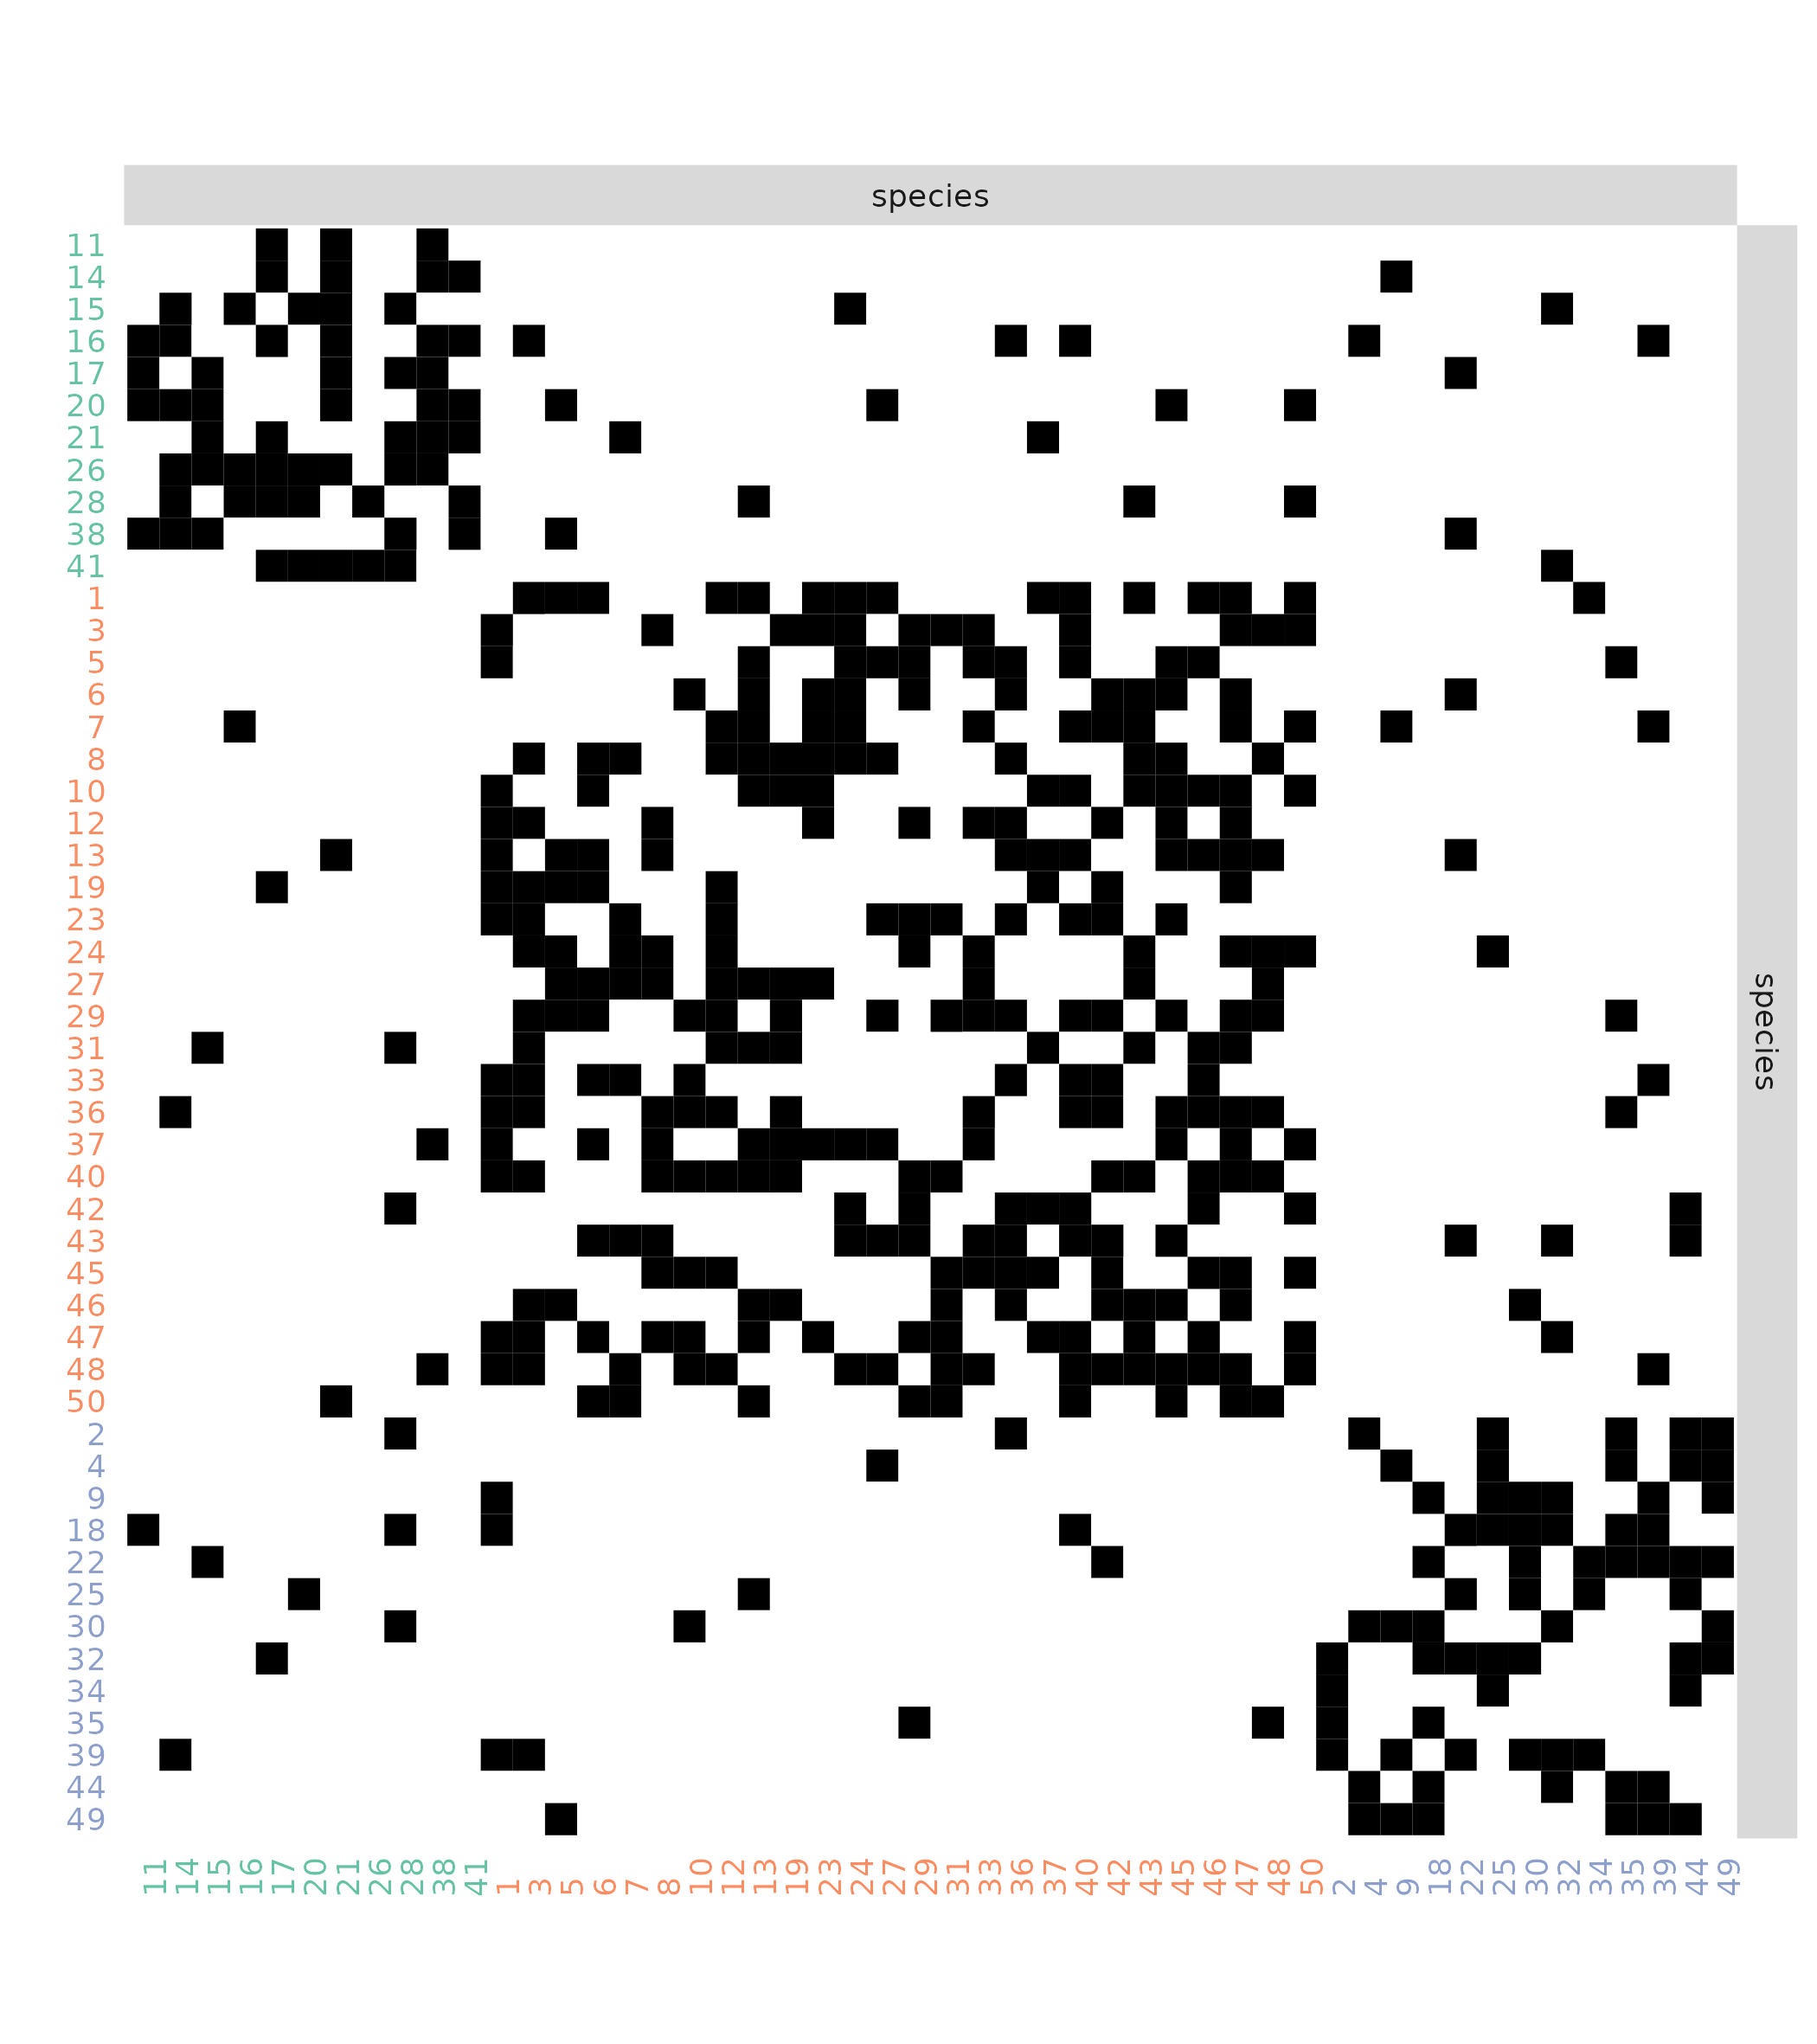
\includegraphics[width=0.5 \textwidth]{plots/matrix_SimuCommunities}

 
\end{frame}

%====================================================================
\begin{frame}\frametitle{Statistical inference}
%====================================================================
\begin{itemize}
\item Selection of the number of clusters 
\begin{itemize}
\item $K$ for SBM ,  $K$ and $L$ for bipartite SBM
\end{itemize}
\item Estimation of the parameters $(\mathbf{\pi}, \btheta)$ for a given number of clusters
\item Clustering $\hat \bZ$
\end{itemize}


Presented in details for binary SBM. 
\end{frame}


%====================================================================
\subsection{Parameters estimation}
%====================================================================
\begin{frame} \frametitle{Likelihood for Bernoulli SBM}
%====================================================================

 \begin{block}{Complete  likelihood $(\bY)$  et  $(\bZ)$}
 \begin{eqnarray}\label{eq:lik}
\ell_c(\bY,\bZ; \theta) &=& p(\bY | \bZ; \balpha) p(\bZ ; \bpi)\nonumber  \\
&=& \prod_{i  \neq j} f_{\alpha_{Z_i,Z_j}}(Y_{ij}) \times   \prod_{i} \pi_{Z_i} \nonumber  \\
&=&  \prod_{i,j} \alpha_{Z_i,Z_j}^{Y_{ij}} (1-  \alpha_{Z_i,Z_j})^{1- Y_{ij}}    \prod_{i} \pi_{Z_i} \nonumber
\end{eqnarray}
 
 \end{block}
 

\begin{block}{Marginal likelihood $(\bY)$}
\begin{equation}\label{eq:vraismarg}
\log \ell(\bY; \theta) =\log \sum_{\bZ \in \boldsymbol{\mathcal{Z}}} \ell_c(\bY,\bZ; \theta) \,.
\end{equation}
 \end{block}
 

 \end{frame}
 

 
 
 

%====================================================================
 \begin{frame}{Marginal likelihood  : remark }
 %====================================================================
 
 $$
\log \ell(\bY; \theta) =\log \sum_{\bZ \in \boldsymbol{\mathcal{Z}}} \ell_c(\bX,\bZ; \theta) \,.
$$
 
  \begin{block}{Remark}
$\boldsymbol{\mathcal{Z}} =   \{1,\dots, K\}^{n}$ \color{dgreen} $\Rightarrow$ \color{black}  when  $K$ and $n$ increase, impossible to compute. 
 \end{block}
 
\color{dgreen} \textbf{Standard tool to maximize the likelihood when latent variables involved} \color{black} : EM  algorithm.  
 
 \end{frame}
 
%====================================================================
 \begin{frame}{From EM to variational EM}
 %====================================================================

 
\begin{block}{Standard EM}
At iteration $(t)$ : 
\begin{itemize}
 \item[$\bullet$]\textbf{Step E}: compute 
 $$ Q(\theta | \theta^{(t-1)}) =   \mathbb E_{\color{dgreen}\bZ | \bX, \theta^{(t-1)} } \left[\log \ell_c(\bY,\bZ; \theta)  \right] $$
 \item[$\bullet$]\textbf{Step M}: 
 $$ \theta^{(t)} = \arg \max_{\theta} Q(\theta | \theta^{(t-1)})$$
 \end{itemize}
% 
%
% 
\end{block}
 
 \end{frame}
%====================================================================
 \begin{frame}[allowframebreaks]{Limitations of standard EM}
%====================================================================
Step $E$ requires the computation of    $ \mathbb E_{\color{dgreen}\bZ | \bX, \theta^{(t-1)} } \left[\log \ell_c(\bX,\bZ; \theta)  \right] $

\begin{itemize}
\item 
 \begin{eqnarray*}\label{eq:lik}
\log \ell_c(\bY,\bZ; \theta) &=& \log \left[\prod_{i \neq j} \alpha_{Z_i,Z_j}^{Y_{ij}} (1-  \alpha_{Z_i,Z_j})^{1- Y_{ij}}  \right] + \log \left[  \prod_{i} \pi_{Z_i}  \right]\nonumber\\
&=& \sum_{i \neq j} \sum_{k,\ell =1}^K {\color{dgreen}Z_{ik}Z_{j\ell}} \left[ Y_{ij} \log \alpha_{k\ell} + (1-Y_{ij}) \log(1-\alpha_{k\ell})\right]  \\
&& + \sum_{i,k=1}^{n,K} Z_{ik}  \log \pi_{k} 
\end{eqnarray*}
with $Z_{ik} = \mathbf{1}_{Z_i = k}$ 

\bigskip 
 \item However, once conditioned by par  $\bX$,  the  $\bZ$ are not independent anymore 
  \end{itemize}
  
   \begin{center}
%   \includegraphics[scale=.3, clip=true, trim=0 335 65 0]{../Figures/HMModel}
  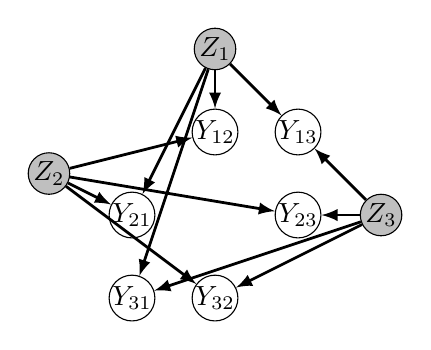
\begin{tikzpicture}
  \node[hidden] (Z1) at (0*\edgeunit, 2*\edgeunit) {$Z_1$};
  \node[hidden] (Z2) at (-2*\edgeunit,  0.5*\edgeunit) {$Z_2$};
 \node[hidden] (Z3) at (2*\edgeunit, 0*\edgeunit) {$Z_3$};

 
  \node[observed] (Y12) at (0*\edgeunit, 1*\edgeunit) {$Y_{12}$};
 \node[observed] (Y13) at (1*\edgeunit, 1*\edgeunit) {$Y_{13}$};
  \node[observed] (Y21) at (-1*\edgeunit, 0*\edgeunit) {$Y_{21}$};

  \node[observed] (Y23) at (1*\edgeunit, 0*\edgeunit) {$Y_{23}$};

  \node[observed] (Y31) at (-1*\edgeunit, -1*\edgeunit) {$Y_{31}$}; 
  \node[observed] (Y32) at (0*\edgeunit, -1*\edgeunit) {$Y_{32}$};


 
  \draw[arrow] (Z1) to (Y12);
  \draw[arrow] (Z1) to (Y21);
  \draw[arrow] (Z1) to (Y31);
  \draw[arrow] (Z1) to (Y13);
  
  \draw[arrow] (Z2) to (Y23);
  \draw[arrow] (Z2) to (Y32);
 
  \draw[arrow] (Z2) to (Y12);
  \draw[arrow] (Z2) to (Y21);
  
  
  \draw[arrow] (Z3) to (Y13);
  \draw[arrow] (Z3) to (Y23);
  \draw[arrow] (Z3) to (Y31);
  \draw[arrow] (Z3) to (Y32);
 
  
  \end{tikzpicture}
  \end{center}
  
$$  p(\bZ | \bX, \theta^{(t-1)}) \neq \prod_{i=1}^n p(Z_i | \bX, \theta^{(t-1)})$$
  
  \end{frame}
%===================

 
%===================
 \begin{frame}{Variational EM  : maximization of a lower bound}
%===================


\textcolor{dgreen}{\textbf{Idea}} : replace the complicated distribution $p(\bZ | \Xall; \theta)$ by a simpler one. 


Let $\mathcal{R}_{\Xall,\btau}$ be any distribution on   $\Zall$


\begin{block}{Central identity}
\begin{eqnarray*}
\mathcal{I}_{\theta}(\mathcal{R}_{\Xall,\btau}) &=& \log \ell(\Xall ; \theta) -   \mathbf{KL}[\mathcal{R}_{\Xall,\btau}, p(\cdot | \Xall; \theta)] \color{dgreen}\quad \leq   \log \ell(\Xall ; \theta)   \\
&=& \mathbb{E}_{\color{dgreen}\mathcal{R}_{\Xall,\btau}} \left[\log \ell_c(\bX,\bZ; \theta)   \right]  -   \sum_{\Zall} \mathcal{R}_{\Xall,\btau}(\bZ)  \log \mathcal{R}_{\Xall,\btau}({\bZ}) \\
&=& \mathbb{E}_{\color{dgreen}\mathcal{R}_{\Xall,\btau}} \left[\log \ell_c(\bX,\bZ; \theta)   \right]  +  \mathcal{H}\left(\mathcal{R}_{\Xall,\btau}(\bZ)\right) 
\end{eqnarray*}
\end{block} 

\textbf{Note that}:  
$$\mathcal{I}_{\theta}(\mathcal{R}_{\Xall,\btau})  = \log \ell(\Xall; \theta) \Leftrightarrow \mathcal{R}_{\Xall,\btau} = p(\cdot | \Xall; \theta)$$ 


\end{frame}

%----------------------------------------------------------------------------------------------
 \begin{frame}[allowframebreaks]{Proof}

By Bayes
\begin{eqnarray*}
\log \ell_c(\bX,\bZ; \theta)&=& \log  p(\bZ | \Xall; \theta) +   \log \ell(\Xall ; \theta)   \\
 \log \ell(\Xall ; \theta) &=& \log \ell_c(\bX,\bZ; \theta) -  \log  p(\bZ | \Xall; \theta)
\end{eqnarray*}

By integration against $\mathcal{R}_{\Xall,\btau}$ : 
\begin{eqnarray*}
 \mathbb{E}_{\color{dgreen}\mathcal{R}_{\Xall,\btau}} [ \log  \ell(\Xall ; \theta)] &=&  \mathbb{E}_{\color{dgreen}\mathcal{R}_{\Xall,\btau}} [\log \ell_c(\bX,\bZ; \theta)] -  \mathbb{E}_{\color{dgreen}\mathcal{R}_{\Xall,\btau}} [ \log  p(\bZ | \Xall; \theta)] \\
 \log \ell(\Xall ; \theta) &=&  \mathbb{E}_{\color{dgreen}\mathcal{R}_{\Xall,\btau}} [\log \ell_c(\bX,\bZ; \theta)] -  \mathbb{E}_{\color{dgreen}\mathcal{R}_{\Xall,\btau}} [ \log  p(\bZ | \Xall; \theta)]
\end{eqnarray*}

As a consequence: 
\begin{eqnarray*}
\mathcal{I}_{\theta}(\mathcal{R}_{\Xall,\btau}) &=& \log \ell(\Xall ; \theta) -   \mathbf{KL}[\mathcal{R}_{\Xall,\btau}, p(\cdot | \Xall; \theta)] \\
 &=& \mathbb{E}_{\color{dgreen}\mathcal{R}_{\Xall,\btau}} [\log \ell_c(\bX,\bZ; \theta)] -  \mathbb{E}_{\color{dgreen}\mathcal{R}_{\Xall,\btau}} [ \log  p(\bZ | \Xall; \theta)]  \\
&& -   \mathbb{E}_{\color{dgreen}\mathcal{R}_{\Xall,\btau}} \left[\log \frac{\mathcal{R}_{\Xall,\btau}(\bZ)} { p(\bZ | \Xall; \theta)}\right]\\
&=&  \mathbb{E}_{\color{dgreen}\mathcal{R}_{\Xall,\btau}} [\log \ell_c(\bX,\bZ; \theta)] -  \mathbb{E}_{\color{dgreen}\mathcal{R}_{\Xall,\btau}} [ \log  p(\bZ | \Xall; \theta)] \\
&& -   \underbrace{\mathbb{E}_{\color{dgreen}\mathcal{R}_{\Xall,\btau}} [\log \mathcal{R}_{\Xall,\btau}(\bZ)]}_{  \mathcal{H}\left(\mathcal{R}_{\Xall,\btau}(\bZ)\right) } +  \mathbb{E}_{\color{dgreen}\mathcal{R}_{\Xall,\btau}} [\log p(\bZ | \Xall; \theta)]
\end{eqnarray*}




  \end{frame}





  %------------------------------------------------------------------------------------------------------
 \begin{frame}{Variational EM }
 

\begin{itemize}
\item Maximization of  $\log \ell(\Xall ; \theta)$  w.r.t.  $\theta$ replaced by maximization of the lower bound $\mathcal{I}_{\theta}(\mathcal{R}_{\Xall,\btau}) $  w.r.t.  $\tau$ and $\theta$. 
\item \textbf{Benefit} : we choose   $\mathcal{R}_{\Xall,\btau}$  such that the maximization calculus can be done explicitly
 \begin{itemize}
 \item In our case: mean field approximation : neglect dependencies between the  $(Z_i)$ 
 $$P_{\mathcal{R}_{\Xall,\btau}}(Z_i=k) = \tau_{ik}$$
  \end{itemize}


  % $\mathcal{R}_{\Xall,\btau}$ approximation of $p(\cdot | \Xall; \theta)$ in a certain class of distributions $\mathcal{P}$

 \end{itemize}
  \end{frame}
%====================================================================
\begin{frame}{Variational  EM}
%====================================================================

\begin{block}{Algorithm}
 \noindent At iteration $(t)$, given the current value  $(\theta^{(t-1)},\mathcal{R}_{\Xall, \btau^{(t-1)}})$,
\begin{enumerate}
\item[$\bullet$]\textbf{Step 1 (VE)} Maximization w.r.t. $\tau$

\begin{eqnarray*}
\btau^{(t)}  &=&  \arg \max_{\btau  \in \mathcal{T}}  \mathcal{I}_{\theta^{(t-1)}}(\mathcal{R}_{\Xall,\btau})\\
 &=&  \arg \max_{\btau  \in \mathcal{T}}   \mathbb{E}_{\color{dgreen}\mathcal{R}_{\Xall,\btau}} \left[\log \ell_c(\bX,\bZ;  \theta^{(t-1)})   \right] +  \mathcal{H}\left(\mathcal{R}_{\Xall,\btau}(\bZ)\right) 
 \end{eqnarray*}
 \end{enumerate}
 \end{block} 
 
Note that 
\begin{eqnarray*}
\btau^{(t)}  &=&  \arg \max_{\btau  \in \mathcal{T}}  \log \ell(\Xall ; \theta^{(t-1)})  -  \mathbf{KL}[\mathcal{R}_{\Xall, \btau}, p(\cdot | \Xall; \theta^{(t-1)})]\\ 
&=& \arg \min_{\btau  \in \mathcal{T}}\mathbf{KL}[\mathcal{R}_{\Xall, \btau}, p(\cdot | \Xall; \theta^{(t-1)})] 
 \end{eqnarray*}
 \end{frame}

%====================================================================
\begin{frame}{Variational  EM}
%====================================================================

\begin{block}{Algorithm}
\begin{enumerate}
 \item[$\bullet$]\textbf{Step 2 (M)} Maximization  w.r.t.  $\theta$
 \begin{eqnarray*}
 \theta^{(t)} &=& \arg \max_{\theta}   \mathcal{I}_{\theta}(\mathcal{R}_{\Xall,\btau^{(t)}}) \\
 &=&   \arg \max_{\theta} \mathbb{E}_{\color{dgreen}\mathcal{R}_{\Xall,\btau^{(t)}}} \left[\log \ell_c(\bX,\bZ;  \theta)   \right]  +   \mathcal{H}\left(\mathcal{R}_{\Xall,\btau^{(t)}}(\bZ)\right)\\
&=&  \arg \max_{\theta} \mathbb{E}_{\color{dgreen}\mathcal{R}_{\Xall,\btau^{(t)}}} \left[\log \ell_c(\bX,\bZ;  \theta)   \right]  
 \end{eqnarray*}
 
\end{enumerate}

 \end{block} 
 \end{frame}
 %====================================================================
 \begin{frame}[allowframebreaks]{Details of the VE-step for binary SBM}
%====================================================================
 
\begin{equation}
 \nonumber
\btau^{(t)} = \arg \min_{\btau}  \mathbf{KL}[\mathcal{R}_{\Xall,\tau}, p(\cdot | \Xall; \theta^{(t-1)})] = \arg \max_{\btau} \mathcal{I}_{\theta^{(t-1)}}(\mathcal{R}_{\Xall,\btau}) \,.
 \end{equation}
(we drop out the index $^{(t-1)}$ on $\theta$)

\begin{eqnarray*}
 \mathcal{I}_{\theta}(\mathcal{R}_{\Xall,\btau}) &=&   \sum_{\bZ} \mathcal{R}_{\Xall,\btau}(\bZ) \log \ell_c(\Xall, \bZ; \theta) -  \sum_{\Zall} \mathcal{R}_{\Xall,\btau}(\bZ)  \log \mathcal{R}_{\Xall,\btau}({\bZ})\,,
 \end{eqnarray*}
 with
 \begin{eqnarray*}
 \log \ell_c(\Xall, \bZ; \theta)% &=& \log p(\Xall |  \bZ; \theta)+ \log  p(\bZ; \theta)\,,\\
 %&=&   \log \prod_{i,j,i\neq j}p(Y_{ij}|  Z_i,Z_j; \theta) + \log \prod_{i=1}^n \alpha_{Z_i}\,,\\
% &=& \sum_{i,j=1, i\neq j}^n  \log p(Y_{ij} |  Z_i,Z_j; \theta)  + \sum_{i=1}^n \log\pi_{Z_i}\,.\\
 &=& \sum_{i,j=1, i\neq j}^n \sum_{k,\ell=1}^K Z_{ik}Z_{j\ell}\log p(Y_{ij} |\alpha_{k\ell})+ \sum_{i=1}^n\sum_{k=1}^K Z_{ik} \log\pi_{k}
 \end{eqnarray*}
 
 
Integration of the $\bZ$ where $\bZ \sim \mathcal{R}_{\Xall,\btau}$% which means that $ \bZ= (Z_i)_{i=1\dots n} $ are independent variables such that $\P(Z_{i}=q) = \tau_{iq}$. We obtain:
 \begin{eqnarray*}
 \mathcal{I}_{\theta}(\mathcal{R}_{\Xall,\btau}) &=& \sum_{i,j=1, i\neq j}^n \sum_{k,\ell=1}^K \tau_{iq}\tau_{j\ell}\log p(Y_{ij} |\alpha_{k\ell})+ \sum_{i=1}^n\sum_{k=1}^K  \tau_{ik} \log\pi_{k} 
 \end{eqnarray*}

 
Maximization under the constraint: $\forall i =1 \dots n$, $\sum_{k=1}^K \tau_{ik}=1$.
 
 
 
\begin{itemize}
 
\item Derivatives of  $$\; \mathcal{I}_{\theta}(\mathcal{R}_{\Xall,\btau})  + \sum_{i=1}^n \lambda_i \left[ \sum_{k=1}^K \tau_{ik}-1\right]$$
 with respect to $(\lambda_i)_{i=1\dots n}$ and $(\tau_{ik})_{i=1\dots n, k=1 \dots K}$ where $\lambda_i$ are the Lagrange multipliers, 
 
 
 
\item Leads  to collection of equations:  for $i=1\dots n$ and $k=1\dots K$,

 \begin{equation}
  \nonumber
 \sum_{\ell=1}^K \sum_{j=1, j\neq i}^n  \log p(Y_{ij} | \alpha_{k\ell})\tau_{j\ell}   +   \log\pi_{k}  -   \log \tau_{ik} +1 + \lambda_i=0\,,
 \end{equation}
 
 \item Leads to the following fixed point problem:

 \begin{equation}
  \nonumber
  \widehat{\tau}_{ik} = e^{1+ \lambda_i} \alpha_k \prod_{j=1, j\neq i}^n \prod_{\ell=1}^K p(Y_{ij} | \alpha_{k\ell}) ^{\widehat{\tau}_{j\ell}}, \quad \forall  i =1 \dots n,  \forall  k=1 \dots K\,,
 \end{equation}
 which has to be solved under the constraints $\forall i =1 \dots n$, $\sum_{k=1}^K \tau_{ik}=1$. This optimization  problem is solved using a  standard fixed point algorithm.

 \end{itemize}
 
 \end{frame}
 
 %====================================================================
 \begin{frame}[allowframebreaks]{Details of the M-step for binary SBM}
%====================================================================

$$\theta^{(t)} = \arg \max_{\theta}   \mathcal{I}_{\theta^{(t)}}(\mathcal{R}_{\Xall, \btau^{(t)}}) $$

under the constraints: $ \sum_{k=1}^k \pi_k=1.$


Maximization with respect to $\bpi$ is quite direct:
$$
\widehat{\pi}_q = \frac{1}{n} \sum_{i=1}^n \widehat{\tau}_{ik}
$$ 
 
For the Bernoulli SBM: 

$$
\widehat{\alpha}_{k\ell} = \frac{\sum_{i,j=1,i\neq j}^n \widehat{\tau}_{ik}  \widehat{\tau}_{j\ell} Y_{ij}}{\sum_{i,j=1,i\neq j}^n  \widehat{\tau}_{ik}  \widehat{\tau}_{j\ell} }
$$

If the edge probabilities depend on covariates:
\begin{equation}
 \nonumber
 \mbox{logit}(p_{k\ell}) = \alpha_{k\ell} +  \beta \cdot x_{ij}\,,
\end{equation}
then the optimization of $ (\alpha_{k\ell})$ and $ (\beta)$ at step M of the VEM is not explicit anymore and one should resort  to optimization algorithms such as Newton-Raphson
algorithm.  
 
 \end{frame}
%====================================================================
\begin{frame}{In practice}
%====================================================================
\begin{itemize}
\item Really fast
\item Strongly depend on the initial values
\end{itemize}

\end{frame}
 
 \subsection{Model selection}
%====================================================================
 \begin{frame}{ Penalized likelihood criterion}
%====================================================================

 \begin{itemize}
 \item  Selection of the number of clusters  $K$ (or $K_1$, $K_2$ in the LBM)
\item   Integrated Classification Likelihood (ICL)   \textcolor{mygreen}{\cite{biernacki2000assessing}}
 

\begin{equation}\label{eq:ICL}
ICL(\M) =\log  \ell_c(\Xall,\hat{\bZ}; \hat \theta_{\bK})-  \pen(\M)
\end{equation}
 where  \begin{equation}\label{eq:Zhat}
\hat{Z}_i = \argmax_{k \in \{1, \dots, K\}}  \hat{\tau}_{ik}. 
\end{equation} 
\item   Integrated Complete Likelihood (ICL)  % \textcolor{mygreen}{\cite{biernacki2000assessing}}

 

\begin{equation}\label{eq:ICL}
ICL(\M) =\mathbb{E}_{p(\cdot | \bY, \hat \theta_{\bK})}[\log  \ell_c(\Xall,\hat{\bZ}; \hat \theta_{\bK})-  \pen(\M)
\end{equation}
 \end{itemize}

\end{frame}


%====================================================================
 \begin{frame}{Expression of the penalization for SBM}
%====================================================================
 
 
\begin{itemize}
 \item For directed network 
 $$ pen_{\mathcal{M}} =
 \frac{1}{2}\left\{ (K-1)\log(n)  +K^2   \log \left( n^2-n \right)\right\} 
$$ 


 \item For undirected network 
$$ pen_{\mathcal{M}} =  \frac{1}{2}\left\{ \underbrace{(K-1)\log(n) }_{\mbox{\textcolor{dgreen}{Clust. }}}  +  \frac{K(K+1)}{2}   \log \left(\frac{ n^2-n }{2}\right)\right\} $$


\end{itemize}
\end{frame}


%====================================================================
 \begin{frame}{Expression of the penalization for bipartite  SBM}
%====================================================================

$$ pen_{\mathcal{M}} =  -  \frac{1}{2}  \left\{  \underbrace{ (K_1-1)\log(n_1) +  (K_2-1)\log(n_2)  }_{\mbox{\textcolor{dgreen}{Bi-Clust. }}} 
  +   \underbrace{ (K_1  K_2)    \log ( n_1   n_2)} _{\mbox{\textcolor{dgreen}{Connection }}} \right\} $$ 


\end{frame}
 

%====================================================================
\begin{frame}{Advantages of ICL}
%====================================================================

 
\begin{itemize}
\item its capacity to outline the clustering structure in networks% in \cite{Daudinetal2008} (for simple networks),  \cite{keribin2015} (for bipartite networks)  or \cite{mariadassou2010} for valued networks.  
\item Involves a trade-off between goodness of fit and model complexity
\item ICL values :   goodness of fit  AND clustering  sharpness.
 
\end{itemize}

\end{frame}

 


 
%====================================================================
 \begin{frame}{Comments on the   ICL versus BIC}
%====================================================================
\begin{block}{Conjecture}
\begin{eqnarray*}
 BIC(\Mcal)  &=&  \log \ell(\Xall; \hat{\theta}, \Mcal) - \mbox{pen}(\Mcal)
\end{eqnarray*}
with the same penalty
 \end{block}

\begin{itemize}
\item Under this conjecture
\begin{eqnarray*}
 ICL(\Mcal)  &= & BIC(\Mcal)  +   \sum_{\Zall} p(\bZ | \Xall;\hat \theta_{\bK}) \log p(\bZ | \Xall; \hat \theta_{\bK})\\
 &=& BIC(\Mcal)  -   \mathcal{H}( p(\cdot | \Xall; \theta)) 
\end{eqnarray*}
\item As a consequence, because of the entropy,  ICL  will encourage clustering with well-separated groups 
\item 
$$ 
 \widehat{ICL}(\mathcal{M})  =BIC(\mathcal{M})  +   \sum_{\Zall} \mathcal{R}_{\Xall}(\bZ,\widehat{\btau})  \log \mathcal{R}_{\Xall,\widehat{\btau}}({\bZ}) -  \mathbf{KL}[\mathcal{R}_{\Xall,\widehat{\btau}}, p(\cdot | \Xall;\widehat{\theta})]\,. 
$$

\end{itemize}

 
 \end{frame}

%====================================================================
\begin{frame}{Algorithm in practice}  
%====================================================================
\begin{itemize}
\item Going trough the models and initiate VEM at the same time
\item Bounds on $K$ :  $\{K_{ \min},\dots, K_{\max}\}$
\end{itemize}

\begin{block}{Stepwise procedure}
Starting from  $K$

\begin{itemize}
\item \textbf{Split} : if $K<K_{\max}$
\begin{itemize}
\item Maximize the likelihood (lower bound) of  $\mathcal{M}_{K+1}$
\item  $K$ initializations of the VEM are proposed :  split each cluster into $2$ clusters  
\end{itemize}
\item \textbf{Merge} :  If $K>K_{\min}$
\begin{itemize}
\item Maximize the likelihood (lower bound) of   model  $\mathcal{M}_{K-1}$
\item  $\frac{K(K-1)}{2}$ initializations of the VEM are proposed :   merging all the possible pairs of  clusters 
 \end{itemize}
\end{itemize}

\end{block}
 \end{frame}


\begin{frame}\frametitle{Theoretical properties for SBM}
\begin{itemize}
\item Identifiability and a first consistency result by \textcolor{mygreen}{\cite{celisse2012consistency} }
\item Consistency of the posterior distribution of the latent variables \textcolor{mygreen}{\cite{mariadassou2015convergence}}
\item Consistency and properties of the variational estimators \textcolor{mygreen}{\cite{bickel2013asymptotic} \color{black}}
\end{itemize}
\end{frame}

%====================================================================
\begin{frame}{Other extensions}
%====================================================================

\begin{itemize}
\item  Time evolving networks \textcolor{mygreen}{Matias} 
\item  Multipartite, Multiplexe networks (\textcolor{mygreen}{R-package  sbm, Bar-Hen, Barbillon, Donnet}) 
\item Multilevel networks (individuals and organizations)  (\textcolor{mygreen}{Chabbert-Liddell})
 \item Missing data in the network \textcolor{mygreen}{\cite{tabouy2019variational}}
\end{itemize}
\end{frame}


%====================================================================
\begin{frame}
 \frametitle{Probabilistic model for networks in a nutshell} 
%====================================================================

 SBM/LBM
 \begin{itemize}
  \item generative models,
  \item flexible,
  \item comprehensive models which can be linked to a lot of classical descriptors.
  
 \end{itemize}
\end{frame}

%====================================================================
\begin{frame}
%====================================================================
\begin{center}

\includegraphics[width=0.5 \textwidth]{plots/PRACTICE-TIME}
\end{center}
  



Comprehensive R package available on CRAN and Github gathering several block models and there in references with vignettes.  

\href{https://grosssbm.github.io/sbm/}{\textcolor{dgreen}{https://grosssbm.github.io/sbm/}}



\vspace{5em}
{ \footnotesize Illustration from \href{http://androiddeveloper.galileo.edu/android-tutorial/time-to-practice-java-for-android-development/}{there}}


\end{frame}




\begin{frame}[allowframebreaks]{References}
\bibliographystyle{apalike}
 \small{\bibliography{biblioSlidesSBM}}
  \end{frame}
  
  
  




\end{document}
